% !TeX program = XeLaTeX
% author: buwailee@nmhs
\documentclass[9pt,twoside,openany,svgnames,x11names]{extbook}
\usepackage[b5paper, top=10mm, text={144mm, 208mm}, includehead, includefoot, hmarginratio=1:1, heightrounded]{geometry}
\usepackage[explicit,clearempty]{titlesec}
\usepackage{wallpaper,changepage,fancyhdr,tikz,indentfirst}
\usepackage{amssymb,amsfonts,amsmath,amsthm,bm,mathrsfs}
\def\pgfsysdriver{pgfsys-dvipdfm.def}
\usepackage[all]{xy}
\usetikzlibrary{shapes,positioning}
\usepackage{hyperref}
	\hypersetup{bookmarksnumbered=true}

%% Command to hold chapter illustration image
\newcommand\chapterimg{Pictures/0.png}

%% Define how the chapter title is printed
\titleformat{\chapter}{}{}{0pt}{
%% Background image at top of page
%% Draw a semi-transparent rectangle across the top
	%% Check if on an odd or even page
	\strictpagecheck\checkoddpage
	\ifoddpage{
	\ThisULCornerWallPaper{1}{\chapterimg}
	}
	\else {
	\newpage
	\thispagestyle{plain}
	\ThisULCornerWallPaper{1}{\chapterimg}
	}
	\fi
	\tikz[overlay,remember picture]
	\fill[opacity=.7]
	(current page.north west) rectangle 
	([yshift=-3cm] current page.north east);
	\begin{tikzpicture}[overlay,remember picture]
	\node[anchor=south west,text=white,
		xshift=20mm,yshift=-25mm,
		font=\sffamily\bfseries\huge] 
		at (current page.north west) 
		{\chaptername\ \thechapter};
	\node[fill=Sienna!80!black,text=white,
		font=\Huge\bfseries, 
		inner ysep=12pt, inner xsep=20pt,
		rounded rectangle,anchor=east, 
		xshift=-20mm,yshift=-30mm] 
		at (current page.north east) {#1};
	\end{tikzpicture}
}
%% Define how the chapter title is printed
\titleformat{name=\chapter,numberless}{}{}{0pt}{
%% Draw a semi-transparent rectangle across the top
\tikz[overlay,remember picture]
	\fill[opacity=.7]
	(current page.north west) rectangle 
	([yshift=-3cm] current page.north east);
	\begin{tikzpicture}[overlay,remember picture]
	\node[fill=Sienna!80!black,text=white,
		font=\Huge\bfseries, 
		inner ysep=12pt, inner xsep=20pt,
		rounded rectangle,anchor=east, 
		xshift=-20mm,yshift=-30mm] 
		at (current page.north east) {#1};
	\end{tikzpicture}
}
\titlespacing*{\chapter}{0pt}{0pt}{100mm}
\titlespacing*{name=\chapter,numberless}{0pt}{0pt}{50mm}

%% Set the uniform width of the colour box
%% displaying the page number in footer
%% to the width of "99"
\newlength\pagenumwidth
\settowidth{\pagenumwidth}{99}

%% Define style of page number colour box
\tikzset{pagefooter/.style={
anchor=base,font=\sffamily\bfseries\small,
text centered,text depth=17mm,text width=\pagenumwidth}}

%% Concoct some colours of our own
\definecolor[named]{GreenTea}{HTML}{000000}

%%%%%%%%%%
%%% Re-define running headers on non-chapter pages
%%%%%%%%%%
\fancypagestyle{headings}{%
	\fancyhf{}   % Clear all headers and footers first
	%% Right headers on odd pages
	\fancyhead[RO]{%
	%% First draw the background rectangles
	%% Then the decorative line and the right mark
	
\begin{tikzpicture}[xshift=-.75\baselineskip,yshift=.25\baselineskip,remember picture,    overlay,fill=GreenTea,draw=GreenTea]\fill circle(3pt);\draw[semithick](0,0) -- (current page.west |- 0,0);\end{tikzpicture} \sffamily\itshape\small\nouppercase{\rightmark}
	}

	%% Left headers on even pages
	\fancyhead[LE]{%
	%% Background rectangles first
	%% Then the right mark and the decorative line
	\sffamily\itshape\small\nouppercase{\leftmark}\ 
	\begin{tikzpicture}[xshift=.5\baselineskip,yshift=.25\baselineskip,remember picture, overlay,fill=GreenTea,draw=GreenTea]\fill (0,0) circle (3pt); \draw[semithick](0,0) -- (current page.east |- 0,0 );\end{tikzpicture}
	}

	%% Right footers on odd pages and left footers on even pages,
	%% display the page number in a colour box
	\fancyfoot[RO,LE]{\tikz[baseline]\node[pagefooter]{\thepage};}
	\renewcommand{\headrulewidth}{0pt}
	\renewcommand{\footrulewidth}{0pt}
}

%%%%%%%%%%
%%% Re-define running headers on chapter pages
%%%%%%%%%%
\fancypagestyle{plain}{%
	%% Clear all headers and footers
	\fancyhf{}
	%% Right footers on odd pages and left footers on even pages,
	%% display the page number in a colour box
	\fancyfoot[RO,LE]{\tikz[baseline]\node[pagefooter]{\thepage};}
	\renewcommand{\headrulewidth}{0pt}
	\renewcommand{\footrulewidth}{0pt}
}
% \usepackage[fontset=windows]{ctex}
\usepackage{ctex}
	% \CTEXoptions[today=old]
	% \CTEXoptions[contentsname=Table of Contents]
% \usepackage[chapter]{../egastyle}

\theoremstyle{definition}
	\newtheorem{para}{}[section]
		\renewcommand{\thepara}{\thesection.\arabic{para}}
	\newtheorem{exa}[para]{Example}
\theoremstyle{plain}
	\newtheorem{lem}[para]{Lemma}
	\newtheorem{theo}[para]{Theorem}
	\newtheorem{thm}[para]{Theorem}
	\newtheorem{pro}[para]{Proposition}
	\newtheorem{coro}[para]{Corollary}
\renewcommand*{\proofname}{Proof}

\usepackage{titletoc, makeidx}
	\makeindex
	% \renewcommand{\indexname}{Index}
\usepackage[titletoc,title]{appendix}
	% \renewcommand{\appendixname}{Appendix}

\usepackage{hyperref,paralist}
	\hypersetup{bookmarksnumbered=true}

\definecolor{shadecolor}{rgb}{0.92,0.92,0.92}

\newcommand{\no}[1]{{$(#1)$}}
% \renewcommand{\not}[1]{#1\!\!\!/}
\newcommand{\rr}{\mathbb{R}}
\newcommand{\zz}{\mathbb{Z}}
\newcommand{\aaa}{\mathfrak{a}}
\newcommand{\pp}{\mathfrak{p}}
\newcommand{\mm}{\mathfrak{m}}
\newcommand{\dd}{\mathrm{d}}
\newcommand{\oo}{\mathcal{O}}
\newcommand{\calf}{\mathcal{F}}
\newcommand{\calg}{\mathcal{G}}
\newcommand{\bbp}{\mathbb{P}}
\newcommand{\bba}{\mathbb{A}}
\newcommand{\osub}{\underset{\mathrm{open}}{\subset}}
\newcommand{\csub}{\underset{\mathrm{closed}}{\subset}}

\DeclareMathOperator{\im}{Im}
\DeclareMathOperator{\Hom}{Hom}
\DeclareMathOperator{\id}{id}
\DeclareMathOperator{\rank}{rank}
\DeclareMathOperator{\tr}{tr}
\DeclareMathOperator{\supp}{supp}
\DeclareMathOperator{\coker}{coker}
\DeclareMathOperator{\codim}{codim}
\DeclareMathOperator{\height}{height}
\DeclareMathOperator{\sign}{sign}

\DeclareMathOperator{\ann}{ann}
\DeclareMathOperator{\Ann}{Ann}
\DeclareMathOperator{\ev}{ev}
	\newcommand{\cc}{\mathbb{C}}
	\DeclareMathOperator{\spec}{Spec}

\begin{document}
\thispagestyle{empty}
%% Cover illustration
	\ThisLLCornerWallPaper{1.1}{../Pictures/1.jpg}
	% Buwai Lee@Shanghai Nanyang Model High School
	\vspace*{2\baselineskip}
	\begin{flushright}
	\includegraphics[scale=0.5]{../Pictures/img1.png}

	\vspace*{1.5\baselineskip}
	{\Huge\bfseries 代数几何笔记}\\[\baselineskip]
	% {{\scshape In\:}\Large {\itshape a simple} {\scshape Way}} \par
	{by Buwai Lee@NJU}\par
	\today
	\end{flushright}
	\vfill
	{\Large\itshape Just for fun}

	\tikz[overlay,remember picture]
 	\fill[opacity=.2]
  	(current page.north west) rectangle 
  	([xshift=-8.3cm, yshift=-11.5cm] current page.east);

	\tikz[overlay,remember picture]
 	\fill[opacity=.7]
  	(current page.south west) rectangle 
  	([yshift=1cm] current page.south east);
	\tikz[remember picture,overlay]%
	\node[font=\LARGE\bfseries,text=Cornsilk,%
	minimum width=\paperwidth,minimum height=3em,anchor=south]%
	 at (current page.south) {解解伟光正出版社};
\clearpage
\frontmatter
\pagestyle{plain}
\ThisULCornerWallPaper{1}{../Pictures/0.png}
\tableofcontents
\mainmatter
\pagestyle{headings}
	% !TEX root = main.tex
\chapter{代数簇}

第一章让我们回顾一下古典的代数簇,它包含了许多代数结论,这些结论将来是用得到的。此外,古典的理论有助于类比现代的理论,所以写下了这章。

\section{仿射簇}

代数簇粗略来说是一族多项式的零点集,他是古典代数几何的主要研究对象。有了它就可以谈论一些代数构造的几何直观。

\begin{para}
假设有一个域$k$,他的代数闭包为$\bar{k}$,定义$n$元有序组$\bba^n_k=\bar{k}\times \cdots \times \bar{k}$为($\bar{k}$上的)$n$维仿射空间,其中的元素被称为点,对一个点$p=(a_1$, $\dots$, $a_n)$中的$a_i$被称为$p$的坐标。如果不是必须写出域$k$,则$n$维仿射空间通常直接写作$\bba^n$.

考虑域$k$上的多项式环$A=k[x_1$, $\dots$, $x_n]$,其中的元素都可以看成函数$f:\bba^n\to \bar{k}$,于是可以定义他的零点集:对于$A$中的一众元素,即一个集合$T$,定义$Z(T)$为$T$的共同零点集,即
\[
Z(T)=\{x\in \bba^n\,:\, \forall f\in T,\, f(x)=0\}.
\]
注意到集合$T$可以生成$A$的一个理想,这个理想的共同零点集和$Z(T)$是一样的。如果$T$是单点集,即只包含一个多项式$f$,此时我们会用$Z(f)$来简记$Z(\{f\})$.

若$\bba^n$中的一个子集$Y$是某个$T$的零点集的时候,即$Z(T)=Y$,此时称$Y$为一个(仿射)代数集。
\end{para}

由于$k$是一个域,所以多项式环$A$是Noether环,他的每个理想都是有限生成的,所以任意的$Z(T)$都可以表示为有限个多项式的共同零点。

\begin{para}
考虑一个$\bba^n$中的子集$Y$,我们可以反过来去找$A$的元素$f$,使得$f$在$Y$中为零,于是定义:$I(Y)$是那些使得$f$在$Y$上为零的函数的集合。容易看出这是一个理想。

令$Y$是一个代数集,定义仿射坐标环为$A(Y)=A/I(Y)$. 从定义来看,$A(Y)$是一个有限生成的$k$-代数。
\end{para}

\begin{pro}下面命题成立:
\begin{compactenum}[~~~(1)]
\item 如果$T_1\subset T_2 \subset A$,则$Z(T_2)\subset Z(T_1)$.
\item 如果$Y_1\subset Y_2 \subset \bba^n$,则$I(Y_2)\subset I(Y_1)$.
\item 如果$\{Y_\alpha\,:\alpha\in I\}$是一族$\bba^n$的子集,则$I\left(\bigcup_{\alpha\in I} Y_\alpha\right)=\bigcap_{\alpha\in I} I(Y_\alpha)$.
\item 如果$\{T_\alpha\,:\alpha\in I\}$是一族$A$的子集,则$Z\left(\bigcup_{\alpha\in I} T_\alpha\right)=\bigcap_{\alpha\in I} Z(T_\alpha)$.
\item $Z(T_1)\cup Z(T_2)=Z(T_1T_2)$.
\item $Y\subset Z(I(Y))$以及$T\subset I(Z(T))$.
\end{compactenum}
\end{pro}

\begin{proof}
	第一第二第六点从定义显然。第三点,由于$Y_\alpha\subset \bigcup_{\alpha\in I} Y_\alpha$,所以由(2)可知$I\left(\bigcup_{\alpha\in I} Y_\alpha\right)\subset\bigcap_{\alpha\in I} I(Y_\alpha)$. 反过来,任取$f\in \bigcap_{\alpha\in I} I(Y_\alpha)$,由于$f\in I(Y_\alpha)$,所以他在每个$Y_\alpha$上为零,故而在$\bigcup_{\alpha\in I} Y_\alpha$上为零。第四点的证明也类似。第五点,对于多项式$f$和$g$有显然的$Z(fg)=Z(f)\cup Z(g)$,然后从第四点得证。
\end{proof}

上面命题的第四第五点验证了代数集满足闭集公理,所以这也就赋予了$\bba^n_k$一个拓扑,称为Zariski拓扑。在这个拓扑下,闭集就是代数集。这个拓扑不一定是Hausdorff的,比如考虑$\bba^1_k$的情况,他的单点集不一定是闭集。但在$k=\bar{k}$的时候,考虑$P=(a_1$, $\dots$, $a_n)$,那么存在理想$(x_1-a_1$, $\dots$, $x_n-a_n)$在$P$上为零,所以此时单点集是闭集。

结合上面命题的第一第二第六点,$A$的理想集和$\bba^n$的子集之间建立了一个Galois联络。而研究这个Galois联络下具体的对应,就是Hilbert's Nullstellensatz的内容\footnote{这是经典代数几何最重要的定理,Nullstellensatz是德文,意思是零点定理。这个定理联系了代数集与多项式环中的理想,可以说确立了几何和代数之间的基本关系,而代数几何正是建立在这一关联的基础之上的。Hilbert零点定理有许多等价形式,而Zariski引理正是其一,下面我们主要使用Zariski引理。},我们下面会慢慢阐述。首先指出一半的内容。

\begin{pro}
如果$Y \subset \bba^n$,则$Z(I(Y))=\overline{Y}$,即$Y$的闭包。
\end{pro}

\begin{proof} 首先,由$Y\subset Z(I(Y))$和$Z(I(Y))$是闭的,所以$\overline{Y}\subset Z(I(Y))$. 反方向,让$\overline{Y}=Z(\mathfrak{a})$,所以$I(Z(\mathfrak{a}))\subset I(Y)$,即$\mathfrak{a}\subset I(Z(\mathfrak{a}))\subset I(Y)$,两边取零点集即$Z(I(Y))\subset Z(\mathfrak{a})=\overline{Y}$. \end{proof}

\begin{coro}
如果一个多项式在$Y$上为$0$当且仅当他在$\overline{Y}$上为$0$. 
\end{coro}

\begin{proof}
即证$I(\overline{Y})=I(Y)$. 将$Z(I(Y))=\overline{Y}$两边取理想,那么$I(\overline{Y})=I(Z(I(Y)))$,特别地,有包含关系$I(Y)\subset I(Z(I(Y)))=I(\overline{Y})$,但是$Y\subset \overline{Y}$又告诉我们$I(\overline{Y})\subset I(Y)$,所以$I(\overline{Y})=I(Y)$.
\end{proof}

\begin{thm}[Zariski引理]
设$k$是一个域,$R$是一个有限生成$k$-代数,如果$R$是一个域,则$R$是$k$的一个有限扩张。
\end{thm}

下面借助Zariski引理,我们来研究$Z(\mm)$和单点集闭包的结构。

\begin{lem}
对任意$A=k[x_1$, $\dots$, $x_n]$中的极大理想$\mm$,$Z(\mm)\neq\varnothing$.
\end{lem}

\begin{proof} 由于$\mm$极大,那么$k[x_1$, $\dots$, $x_n]/\mm=k[\bar{x}_1$, $\dots$, $\bar{x}_n]$就是一个域,由Zariski引理,他是$k$的一个有限扩张。设$\bar{x}_i$是$x_i$在$k[x_1$, $\dots$, $x_n]/\mm$里面的像,由于是代数扩张,所以$\bar{x}_i\in \bar{k}$. 此时$\mm$中的多项式至少有公共零点$(\bar{x}_1$, $\dots$, $\bar{x}_n)\in \bba^n$,因为对任意$f\in \mm$都成立
\[
	f(\text{$\bar{x}_1$, $\dots$, $\bar{x}_n$})=\sum a_{i_1\cdots i_n} {\bar{x}}_1^{i_1}\cdots {\bar{x}}_n^{i_n}=\overline{\sum a_{i_1\cdots i_n} x_1^{i_1}\cdots x_n^{i_n}}=\bar{f}=0.
\]
所以这就推出了$Z(\mm)\neq\varnothing$.
\end{proof} 

实际上,$Z(\mm)$中元素的个数与Galois群$\Gal(A(\mm)/k)$中元素的个数是相同的(因此有限),因为$Z(\mm)$可以理解成Galois群$\Gal(A(\mm)/k)$在$\bba^n$上的一条轨道。这里我们就不证明这点了。

\begin{lem}
每一个极大理想的零点集是极小非空闭集,每一个极小的非空闭集都是某个唯一的极大理想的零点集。
\end{lem}

而由拓扑的知识我们知道,极小的闭集是单点集的闭包,所以多项式环的极大理想一一对应着Zariski拓扑中单点集的闭包(其实这也是不可约闭子集)。

\begin{proof}
设$\mm$是$A$的极大理想,此时$Z(\mm)$非空,所以理想$I(Z(\mm))$不是单位理想,由$\mm\subset I(Z(\mm))$,可知$I(Z(\mm))=\mm$. 因此,如果$\mm_1$, $\mm_2$是两个极大理想满足$Z(\mm_1)=Z(\mm_2)$,则$\mm_1=\mm_2$.

现在如果有一个$Z(\mathfrak{a})=\varnothing$满足$Z(\mathfrak{a})\subset Z(\mm)$,两边取理想得到$\mm\subset I(Z(\mathfrak{a}))$,由于$\mm$极大,所以$\mm = I(Z(\mathfrak{a}))$. 两边取一次零点集将得到$Z(\mm)=Z(I(Z(\mathfrak{a})))$,所以$Z(\mathfrak{a})\subset Z(I(Z(\mathfrak{a})))=Z(\mm)$,故$Z(\mm)=Z(\mathfrak{a})$.

反过来,对于一个极小非空闭集$Y=Z(\mathfrak{a})$,它的理想集为$I(Z(\mathfrak{a}))$. 取$\mathfrak{m}$为包含$I(Z(\mathfrak{a}))$的任意极大理想,由Galois联络,$Z(\mathfrak{m})\subset Z(I(Y))=Y$,由极小性,$Y=Z(\mathfrak{m})$. 唯一性前面已经证明。
\end{proof}
\

最后来谈谈反问题,前面已经看到,对于任意的极大理想,他的零点集非空。反过来,对于一个任意单点$P\in \bba^n_k$,我们想要寻找极大理想,使得$P$是他的公共零点。存在性是简单的,对于任意点$P\in \bba^n_k$,因为他的闭包就是极小的闭集,对应着一个极大理想$I(\overline{\{P\}})$. 下面的命题保证了唯一性。

\begin{pro}
若$P\in \overline{\{Q\}}$,则$\overline{\{P\}}= \overline{\{Q\}}$.
\end{pro}

\begin{proof}
将$\overline{\{P\}}\subset \overline{\{Q\}}$取理想得到$I(\overline{\{Q\}})\subset I(\overline{\{P\}})$,因为这是两个极大理想,所以$I(\overline{\{Q\}})=I(\overline{\{P\}})$. 两边再取零点集,则
\[
	Z\left(I(\overline{\{Q\}})\right)=Z\left(I(\overline{\{P\}})\right).
\]
利用$Z(I(Y))=\overline{Y}$,所以$\overline{\{P\}}= \overline{\{Q\}}$. 
\end{proof}

现在我们来看一般的$Z(\mathfrak{a})$. 对于闭集$\overline{\{P\}}\subset Z(\mathfrak{a})$,在$A$中可以找到唯一的极大理想$I(\overline{\{P\}})$,满足
$\mathfrak{a}\subset I(Z(\mathfrak{a}))\subset I(\overline{\{P\}})$. 反过来,任取一个包含$\mathfrak{a}$的极大理想$\mm$,由于$\mathfrak{a}\subset \mm$,所以$Z(\mm)\subset Z(\mathfrak{a})$. 而$Z(\mm)$正是一个$\overline{\{Q\}}$. 所以$Z(\mathfrak{a})$中单点集的闭包一一对应着包含$\mathfrak{a}$的极大理想,这个观察给出了下面一个命题。

\begin{pro}
如果$\mathfrak{a}$是$A$的一个理想,则$I(Z(\mathfrak{a}))=\sqrt{\mathfrak{a}}$.
\end{pro}

这个命题也被称为Hilbert's Nullstellensatz. 对于任意满足$\mathfrak{a}=\sqrt{\mathfrak{a}}$的理想(称为根式理想),有$I(Z(\mathfrak{a}))=\mathfrak{a}$. 这个命题给出了明确的Galois联络两边的像,即根式理想与代数集一一对应。

\begin{proof} 由于$Y=Z(\mathfrak{a})$是一个代数集,遍历其中所有的点的闭包,我们有
\[
	I(Z(\mathfrak{a}))=I\left(\bigcup_{P\in Y}\overline{\{P\}}\right)=\bigcap_{P\in Y}I\left(\overline{\{P\}}\right),
\]
注意到单点集的闭包一一对应着包含$\mathfrak{a}$的极大理想,所以$I(Z(\mathfrak{a}))=\bigcap_{\mm\supset \mathfrak{a}}\mm$. 因为$k[x_1$, $\dots$, $x_n]$是Jacobson环,所以$I(Z(\mathfrak{a}))=\sqrt{\mathfrak{a}}$.
\end{proof}

称拓扑空间$X$是不可约的,即是说$X$不能写作它的两个非空真闭子集的并。在不可约空间内,一个开集必然是稠密的,否则他的闭包和他的补集的并构成了全集。可以证明,这样的开集自身也是不可约的。如果$Y$是$X$的不可约子集,那么$Y$的闭包也是$X$的不可约子集。这些都容易构造出两个闭集来证明。

\begin{para}
$\bba^n$中的不可约闭子集被称为一个仿射(代数)簇(affine variety),或者说是$\bba^n$中的不可约代数集。一个仿射簇的开子集被称为是拟仿射(代数)簇。
\end{para}

下面这个命题可以使我们可以看到不可约代数集和素理想之间的联系:

\begin{pro}
一个代数集$Y$是不可约的当且仅当$I(Y)$是一个素理想。
\end{pro}

\begin{proof} 令$\pp$是一个素理想,以及假设$Z(\pp)=Y_1\cup Y_2$,那么$\pp=I(Z(\pp))=I(Y_1)\cap I(Y_2)$,因此$\pp=I(Y_1)$或者$\pp=I(Y_2)$,因此$Z(\pp)$不可约。

反之,假设$Y$不可约,那么如果$fg\in I(Y)$,此时$Y\subset Z(fg)=Z(f)\cup Z(g)$,因此
\[
	Y=[Y\cap Z(f)]\cup [Y\cap Z(g)],
\]
所以$Y=Y\cap Z(f)$或$Y=Y\cap Z(g)$,即$Y\subset Z(f)$或者$Y\subset Z(g)$,即$f\in I(Y)$或者$g\in I(Y)$.因此$I(Y)$是素理想。\end{proof}

对于不可约代数集,$I(Y)=\pp$是一个素理想,所以也是根式理想,他与它的零点集一一对应,即$Y=Z(\pp)$. 所以上面的命题告诉我们,不可约代数集与$A=k[x_1$, $\dots$, $x_n]$的素理想一一对应。

\begin{lem}
	令$Z(f)$是$\bba^n_k$中的超曲面,那么拟仿射簇$\bba^n_k-Z(f)$同构于$\bba^{n+1}_{k}$中的$Z(x_{n+1}f-1)$,所以$\bba^n_k-Z(f)$仿射,且他的坐标环为$k[x_1$, $\dots$, $x_n]_f$,即$k[x_1$, $\dots$, $x_n]$关于$\{1$, $f$, $f^2$, $\dots\}$的分式环。
\end{lem}
\begin{proof}
	设$\varphi:Z(x_{n+1}f-1)\to \bba^n_k-Z(f)$是前$n$个坐标的投影函数,这是一个态射。很清楚,$\varphi$给出了$Z(x_{n+1}f-1)$到$\bba^n_k-Z(f)$的双射,为了证明$\varphi$是一个同构,所以需要证明$\varphi^{-1}$是一个态射。然而$\varphi^{-1}(a_1$, $\dots$, $a_n)=(a_1$, $\dots$, $a_n,1/f(a_1$, $\dots$, $a_n))$,使用Lemma \ref{c3:l1} 就知道这是一个态射。于是$\bba^n_k-Z(f)$仿射,他的坐标环就是$Z(x_{n+1}f-1)$的坐标环,即$k[x_1$, $\dots$, $x_n]_f$.
\end{proof}

\section{射影簇}

定义射影空间$\bbp^n=(\bba^{n+1}-\{0\})/\sim$ ,等价关系是由
\[
(x_0,\dots,x_n)\sim (px_0,\dots,px_n), \quad \forall p\in \bar{k}-\{0\}
\]
确定的等价类$[x_0$, $\dots$, $x_n]$. 多项式环$k[x_1$, $\dots$, $x_n]$记作$S$,齐次多项式构成的子环记作$S^{\mathrm{h}}$.

多项式环$S$是一个分次环,他可以写成分解$S=\bigoplus_{d\geq 0} S_d$,其中$S_d$是由$0$和所有$d$次齐次多项式所并而成的子环。$S$的齐次理想$\mathfrak{a}$是指$S$的由齐次元素生成的理想,齐次理想的元素不一定是齐次的,因为一个齐次理想可以是两个或多个不同次的齐次元素生成的,他们的和一般不是齐次的。齐次理想的乘积、和、交、根式都是齐次的。不加证明地指出,对于齐次理想,成立
\[
	\mathfrak{a}=\bigoplus_{d\geq 0} (\mathfrak{a}\cap S_d).
\]
所以如果一个齐次理想是素理想,只要指出对于任意两个齐次元素$f$, $g$,$fg\in \mathfrak{a}$可以推出$f\in \mathfrak{a}$或$g\in \mathfrak{a}$.

在射影空间上不能well define多项式,但是可以指出,齐次多项式的零点是well defined. 所以一样地,可以定义对于齐次多项式的集合$T$,他的零点集$Z(T)$.

\begin{para}
	一个$\bbp^n$中的子集称为代数集如果他是某些齐次多项式的零点集。
\end{para}
相似地(连证明过程),零点集的性质满足闭集公理,所以$\bbp^n$上也可以用零点集赋予拓扑,依旧将其称为Zariski拓扑。

\begin{para}
	如果$Y$是$\bbp^n$中的子集,定义$S$的齐次理想$I(Y)$为在$Y$上为$0$的齐次多项式生成的理想。$S(Y)=S/I(Y)$被称为齐次坐标环。
\end{para}

\begin{pro}[homogeneous Nullstellensatz]
设$\mathfrak{a}\subset S$是一个齐次理想,则如下命题成立:

\no{1} 设$f\in S_d$且$d>0$,如果$f$在$Z(\mathfrak{a})$上为零,那么$f \in \sqrt{\mathfrak{a}}$.

\no{2} 如果$Z(\mathfrak{a})\neq \varnothing$,则$I(Z(\mathfrak{a}))=\sqrt{\mathfrak{a}}$.
\end{pro}
\begin{proof}
	假设我们有一个闭集$Z(\mathfrak{a})\in \bbp^n$,我们在$\bba^{n+1}$中构造
	\[
		\bar{Z}(\mathfrak{a})=\bigl\{p\in \bba^{n+1}:\forall g\in \mathfrak{a},\, g(p)=0\bigr\},
	\]
	这样$Z(\mathfrak{a})=\bar{Z}(\mathfrak{a})/\sim$,由Hilbert's Nullstellensatz,如果一个多项式$f$,特别地一个齐次多项式,在$\bar{Z}(\mathfrak{a})$上为$0$,则$f\in \sqrt{\mathfrak{a}}$,而齐次多项式在$\bar{Z}(\mathfrak{a})$上为$0$等价于他在$Z(\mathfrak{a})$上为$0$,第一部分搞定。

	第二部分显然我们只要证明$I(Z(\mathfrak{a}))\subseteq \sqrt{\mathfrak{a}}$,这是第一部分的推论。如果$Z(\mathfrak{a})$非空,那么在$Z(\mathfrak{a})$上为$0$的齐次多项式$f\in S_d$必须$d>0$,那么第一部分就表明了反向包含。
\end{proof}

\begin{pro}
	下面命题对于射影的情况依然成立:

	\no{1} 如果$T_1\subseteq T_2 \subseteq S^{\mathrm{h}}$,则$Z(T_2)\subseteq Z(T_1)$.

	\no{2} 如果$Y_1\subseteq Y_2 \subseteq \bbp^n$,则$I(Y_2)\subseteq I(Y_1)$.

	\no{3} 如果$Y_1$, $Y_2 \subseteq \bbp^n$,则$I(Y_1\cup Y_2)=I(Y_1)\cap I(Y_2)$.

	\no{4} 如果$Y \subseteq \bbp^n$,则$Z(I(Y))=\overline{Y}$.
\end{pro}

除了最后一点都是显然的,但是靠着homogeneous Nullstellensatz,和仿射情况的证明几乎没有区别,这里略去。所以,由Nullstellensatz,射影情况下依然成立$I(Y)=I(\overline{Y})$. 类似的命题还有:

\begin{pro}
	一个代数集$Y$是射影簇当且仅当$I(Y)$是一个齐次素理想。
\end{pro}
% \begin{pro}
% 	$\bbp^n$是Noetherian拓扑空间。
% \end{pro}
% 这些命题的证明和仿射的都类似。由于$\bbp^n$是Noetherian拓扑空间,作为他的子集,任何的射影簇和拟射影簇都是Noetherian拓扑空间。

下面的几个命题指出,射影空间实际上被仿射空间开覆盖。

在$\bbp^n$中的第$i$个坐标为$0$的点构成一个子集$H_i$,故而都是闭集,令$U_i=\bbp^n-H_i$,他们都是开集,更进一步,$U_i$是$\bbp^n$的开覆盖,因为如果$p\in \bbp^n$,那么$p$至少有一个坐标$p_i$不为$0$,所以$p\in U_i$.定义映射
\[
	\begin{array}{lccl}
		\varphi_i:&U_i&\to& \bba^n_k\\
		&[a_0,\dots ,a_n]&\mapsto&\displaystyle{\left(\frac{a_0}{a_i},\dots ,\frac{a_{i-1}}{a_i},\frac{a_{i+1}}{a_i},\dots,\frac{a_n}{a_i}\right)}
	\end{array}
\]
这是well defined,因为$a_j/a_i$不依赖于等价类中代表元的选取。

\begin{pro}
$\varphi_i$是$U_i$和$\bba^n_k$在两边各自的Zariski拓扑下的同胚。
\end{pro}
\begin{proof}
双射显然,只要证明$U_i$的闭集被$\varphi_i$等同于$\bba^n_k$中的闭集就可以了。不妨将$i$取做$0$,将$U_i$简记为$U$,$\varphi_i$简记为$\varphi$.

一个齐次多项式$f(x_0$, $x_1$, $\dots$, $x_n)$可以通过$g(x_1$, $\dots$, $x_n)=f(1,x_1$, $\dots$, $x_n)$定义一个$A$中的多项式,我们记作$g=\alpha(f)$.反之,一个最高次为$N$次的多项式$g(x_1$, $\dots$, $x_n)$可以定义一个$N$次齐次多项式$f(x_0$, $x_1$, $\dots$, $x_n)=x_0^Ng(x_1/x_0$, $\dots$, $x_n/x_0)$,我们记作$f=\beta(g)$.

现在令$Y$是$U$中的一个闭子集,令$\overline{Y}$是他在$\bbp^n$中的闭包,$\overline{Y}$是一个闭子集,所以$\overline{Y}=Z(T)$,令$T'=\alpha(T)$,直接的验算可以知道$\varphi(Y)=Z(T')$,所以$\varphi(Y)$是闭集。

反之,令W是$\bba^n_k$中的闭子集,那么$W=Z(T')$,其中$T'$是$A$中的一个自己,直接的验算可以得到$\varphi^{-1}(W)=Z(\beta(T'))\cap U$,所以$\varphi^{-1}(W)$是闭集。
正反的连续性都证毕。所以是同胚。
\end{proof}
\begin{pro}
	如果$Y$是(拟)射影簇,那么$Y$被拟射影簇$\{Y_i=Y\cap U_i\}$开覆盖,且每个拟射影簇$Y_i$通过$\varphi_i$同胚于一个(拟)仿射簇。
	\label{c2:p8}
\end{pro}
\begin{proof}
因为$Y_i=Y\cap U_i$是$Y$中的开集,而$Y$是不可约的,所以$Y_i$是不可约的,由同胚,$\varphi_i(Y_i)$是不可约的。对于(拟)射影的情况,因为$Y$是(开)闭的,所以$Y_i$在$U_i$中是(开)闭的,由同胚,$\varphi_i(Y_i)$在$\bba^n$中是(开)闭的。
\end{proof}

% 因为$U_i$构成$\bbp^n$的开覆盖,利用Proposition \ref{p1.9},则
% \[
% 	\dim  \bbp^n=\sup(\dim U_i)=\max(\dim U_i).
% \]
% 第二个等号来自于覆盖是有限的。但是$U_i$和$\bba^n_k$同胚,所以$\dim U_i=\dim \bba^n_k=n$,因此$\dim  \bbp^n=n$.

% 射影空间的Zariski拓扑依然使得下面命题成立,技术上依然是Proposition \ref{p1.9}:
% \begin{pro}如果$Y$是拟射影簇,那么$\dim Y=\dim \overline{Y}$.\end{pro}
% \begin{proof}
% 设$W_i=\varphi_i(Y\cap U_i)$. 因为$Y$是拟射影簇,所以$W_i$是拟仿射簇。让$\overline{Y}$是$Y$在$\bbp^n$中的闭包,再设$Z_i=\varphi_i(\overline{Y}\cap U_i)$,由于是同胚,$Z_i$是$W_i$的闭包,所以由拟射影簇的结论,$\dim Z_i=\dim W_i$.最后
% \[
% 	\dim Y=\max(\dim Y_i)=\max(\dim W_i)=\max(\dim Z_i)=\dim \overline{Y}.
% \]
% \end{proof}

\section{代数簇及其态射}

前面说了代数簇,但是没有描述代数簇之间的映射。这里就干这活,后面将会看到,代数簇构成一个范畴,而他又和$k$-代数范畴之间有着密不可分的关系。至少就仿射簇来说,一个$k$-代数如果和某个$\bba^n$中的坐标环同构,当且仅当他是有限生成的且没有幂零元。

假设$Y$是$\bba^n$中的拟仿射簇。
\begin{para}
	一个函数$f:Y\to \bar{k}$在点$p\in Y$是正则的,就是说存在$p$的邻域$U$使得$p\in U\subseteq Y$,存在两个多项式$g$, $h$,且$h$在$U$上处处不为$0$,使得$f=g/h$. 称一个函数在$Y$上正则,就是说他在$Y$上的每一点都正则。
\end{para}
\begin{pro}
正则函数是连续的,其中$\bar{k}$被看作$\bba^1$,即被赋予了Zariski拓扑。
\end{pro}
\begin{proof}
	按连续的定义,只要证闭集的逆象是闭的就好了。由于$\bba^1$中的闭集都是有限集,如果我们证明了单点集的逆象是闭的,那也就证明了所有闭集的逆象是闭的。

	闭集可以局部检查,如果$Z$是拓扑空间$Y$的子集,那么他是闭集当且仅当对于任意一个$Y$的开覆盖$\{U_\alpha\}$,$Z\cap U_\alpha$是$U_\alpha$中的闭集。

	找个开覆盖,在每个$U_\alpha$中,$f$都可以写作$f=g_\alpha/h_\alpha$,此时
	\[
		f^{-1}(a)\cap U_\alpha=\bigl\{p\in U| g_\alpha(p)/h_\alpha(p)=a\bigr\},
	\]
	所以$g_\alpha(p)/h_\alpha(p)=a$又等价于$g_\alpha(p)-ah_\alpha(p)=0$,所以
	\[
		f^{-1}(a)\cap U_\alpha=Z(g_\alpha-ah_\alpha)\cap U_\alpha
	\]
	是一个闭集。
\end{proof}
这个证明中告诉我们,对于正则函数,$\bar{k}$上单点集的原像是闭的。这个内容在代数闭域上和连续性是等价的,因为当$k$是代数闭的时候,$\bar{k}$上单点集是闭集,命题说明了正则函数是连续的,所以单点集的原像是闭的。但是到了非代数闭的情况,单点集的原像是闭集所包含的内容是大于连续性的,因为$\bar{k}$上单点集一般不是闭集。

假设$Y$是$\bbp^n$中的拟射影簇,正则的定义非常类似拟仿射簇。
\begin{para}
	一个函数$f:Y\to \bar{k}$在点$p\in Y$是正则的,就是说存在$p$的邻域$U$使得$p\in U\subseteq Y$,存在两个次数相同的齐次多项式$g$, $h$,且$h$在$U$上处处不为$0$,那么$f=g/h$. 称一个函数在$Y$上正则,就是说他在$Y$上的每一点都正则。
\end{para}
相同次数的要求保证了正则函数确实是一个函数。此外,我们一模一样地证明正则函数是连续的。不管是仿射还是射影的,如果$f$和$g$是代数簇$Y$上的正则函数,如果$f$和$g$在$Y$的某个开子集$U$上相同,则他在$Y$上相同。因为
\[
	U\subseteq (f-g)^{-1}(0)\subseteq Y,
\]
因为单点集关于正则函数的原像是闭的,所以$(f-g)^{-1}(0)$是闭集,再由于$U$稠密,两边取闭包就有
\[
	Y\subseteq (f-g)^{-1}(0)\subseteq Y,
\]
所以$(f-g)^{-1}(0)=Y$,就是说,他们在整个$Y$上是相同的。
\begin{para}
令$k$是域,一个代数簇可以指射影、仿射、拟射影、拟仿射簇,所以代数簇的开子集都是代数簇。代数簇范畴的对象就是这些代数簇,剩下的,就是定义这些对象之间的态射。假设$X$, $Y$是两个代数簇,他们之间的连续映射$\varphi:X\to Y$如果满足,对任意的开集$V\subseteq Y$以及$V$上的正则函数$f$,拉回$\varphi^*:f\mapsto f\circ \varphi$后的函数$\varphi^* f=f\circ \varphi:\varphi^{-1}(V)\to \bar{k}$是一个$\varphi^{-1}(V)$上的正则函数,则这个连续映射就是代数簇之间的态射。
\end{para}

态射的复合依然是态射,所以代数簇就构成一个范畴。代数簇范畴的同构就是说,对于态射$\varphi:X\to Y$,存在$\psi:Y\to X$满足$\varphi\circ \psi=\mathrm{id}_Y$以及$\psi\circ \varphi=\mathrm{id}_X$. %由于每一个代数簇(射影、仿射、拟射影、拟仿射簇)都是一个Noetherian拓扑空间,所以每一个代数簇都是紧的。

\begin{pro}
	令$X$是代数簇,在每一点$p\in X$,他的任意开邻域$U$里面都可以找到一个开的仿射集$V$使得$p\in V\subseteq U$.
\end{pro}

这个命题说明了在任意代数簇上,开的仿射子集\footnote{自此以后,我们称一个代数簇是仿射的,如果他同构于一个仿射簇。}将构成一组拓扑基。所以,如果我们在局部考虑问题,很大程度上就是在仿射簇上考虑问题。

\begin{proof}
	因为$U$也是一个代数簇,所以不妨令$U=X$. 其次,按照Proposition \ref{c2:p8},$X$被拟仿射集开覆盖,所以我们可以假设$X$是一个$\bba^n_k$中的拟仿射簇。

	任取$p\in X$,我们来找一个他的仿射邻域。由于$\overline{X}-X$是$\bba^n_k$中的闭集,如果$p\notin \overline{X}-X$,我们可以找到一个不可约多项式$f\in I(\overline{X}-X)$使得$f(p)\neq 0$. 显然$\overline{X}-X\subseteq Z(f)$但$p\notin Z(f)$,所以$p\in X-X\cap Z(f)$,而$X-X\cap Z(f)$是一个$X$中的开集。并且,由$X$是不可约的以及$X-X\cap Z(f)$是一个$X$的开子集,则$X-X\cap Z(f)$是一个不可约集。

	此外,$X-X\cap Z(f)$是一个$\bba^n_k-Z(f)$的闭子集,由上一个引理,$\bba^n_k-Z(f)$仿射,而$X-X\cap Z(f)$是一个仿射集的不可约闭子集,所以也是一个仿射集。于是$X-X\cap Z(f)$是$p$的一个仿射邻域。
\end{proof}

下面这个引理给出了某些情况下的态射的判断方法。
\begin{lem}
	令$X$是一个代数簇,以及$Y$是一个仿射簇,$\psi:X\to Y$是态射当且仅当$\{x_i\circ \psi\}$在$X$上是正则函数,其中$\{x_i\}$是$\bba^n_k$上的坐标函数。
	\label{c3:l1}
\end{lem}
这个判据可以如下表述:$\psi=(f_1,\cdots,f_n)$是一个态射,当且仅当$\{f_i\}$都是$X$上的正则函数。
\begin{proof}
	如果$\psi$是态射,显然$\{\psi^*x_i=x_i\circ \psi\}$在$X$上是正则函数。反之,设$\{\psi^*x_i\}$在$X$上是正则函数,那么对任意多项式$f=f(x_1,\cdots,x_n)$,$\psi^*f$在$X$上依然是正则函数。

	任取$Y$中的闭集$W$,因为$Y$中的闭集是一些多项式的零点集$W=Z(f_1,\cdots,f_k)$(这是因为闭集中闭集依然是在大的空间中是闭集),如果希望证明$\psi$是连续函数,只要证明$\psi^{-1}(W)$是闭集就可以了。因为对于任意的多项式$f$,$\psi^*f=f\circ \psi$在$X$上依然是正则函数,所以$(f\circ \psi)^{-1}(0)=\psi^{-1}(f^{-1}(0))$是闭集,所以
	\[
		\psi^{-1}(W)=\psi^{-1}\left(\bigcap_{i=1}^k f_i^{-1}(0)\right)=\bigcap_{i=1}^k\psi^{-1}\left( f_i^{-1}(0)\right)
	\]
	是有限闭集之交,所以也是一个闭集。

	除去连续性,另外需要证明的是$Y$的任意子集$V$上的正则函数变成了$\psi^{-1}(V)$上的正则函数。由于$V$上任意的正则函数$f$,可以在$V$的任意一点$p$附近写作$f=g_p/h_p$,那么
	\[
		\psi^*f=f\circ \psi=\frac{g_p(x_1\circ \psi,\cdots,x_n\circ \psi)}{h_p(x_1\circ \psi,\cdots,x_n\circ \psi)}=\frac{\psi^*g_p}{\psi^*h_p}.
	\]
	由于$\psi^*g_p$和$\psi^*h_p$在点$\psi^{-1}(p)$的每一点$q$都正则,我们可以找一个$q$的邻域$U\subseteq \psi^{-1}(V)$,在上面$\psi^*g_p$和$\psi^*h_p$都可以写作两个多项式的商,通分后,他们的商还是可以写作两个多项式的商,因此$\psi^*f$在点$q$也是正则的。因为$q$是$\psi^{-1}(p)$中的任意点,$p$是$V$中的任意点,所以$\psi^*f$在$\psi^{-1}(V)$上正则。

	综合上面两点,$\psi$是一个态射。
\end{proof}

以前说过,对于射影空间,有同胚$\varphi_i:U_i\to \bba^n_k$,有了态射的概念,有了代数簇范畴,下面一个命题就说明这还是一个同构。
\begin{pro}
	$\varphi_i:U_i\to \bba^n_k$是一个两个代数簇之间的同构。
	\label{c3:p1}
\end{pro}
\begin{proof}
	既然已经知道是同胚,只要检验正则函数那部分就好。不妨假设$i=0$,记$\varphi=\varphi_0^{-1}$,在$U_i$上的正则函数某个开集$V$上可以写作两个同次齐次多项式的商
	\[
		f\bigl([x_0,\cdots,x_n]\bigr)=\frac{g(x_0,\cdots,x_n)}{h(x_0,\cdots,x_n)},
	\]
	对应着$\varphi^*f$仿射空间内$\varphi_0(V)$处上可以写作
	\[
		\varphi^*f(x_1,\cdots,x_n)=\frac{\alpha(g)(x_1,\cdots,x_n)}{\alpha(h)(x_1,\cdots,x_n)}=\frac{g(1,\cdots,x_n/x_0)}{h(1,\cdots,x_n/x_0)},
	\]
	反过来,对于仿射空间内的正则函数,在$\varphi_0(V)$处上可以写作$j=k/l$,对应着在射影空间内$V$上写作
	\[
		(\varphi^{-1})^*j\bigl([x_0,\cdots,x_n]\bigr)=\frac{x_0^Nk(x_1/x_0,\cdots,x_n/x_0)}{x_0^Nl(x_1/x_0,\cdots,x_n/x_0)}=\frac{\beta(k)(x_0,\cdots,x_n)}{\beta(l)(x_0,\cdots,x_n)}.
	\]

	因此
	\[
		(\varphi^{-1})^*\circ \varphi^*(f) \bigl([x_0,\cdots,x_n]\bigr)=(\varphi^{-1})^*\left(\frac{\alpha(g)}{\alpha(h)}\right)=\frac{\beta(\alpha(g))}{\beta(\alpha(h))}=\frac{g}{h}=f\bigl([x_0,\cdots,x_n]\bigr).
	\]
	所以$\varphi^*\circ(\varphi^{-1})^* (f)=f$,同理可以检验$(\varphi^{-1})^*\circ\varphi^* (j)=j$,所以$\varphi$是一个代数簇之间的同构。
\end{proof}

对于任意的代数簇,可以引入一个函数环,他是仿射情况的坐标环的推广。
\begin{para}
	设$Y$是一个代数簇,记$\mathcal{O}(Y)$是所有$Y$上的正则函数按照加法和乘法构成的环。
\end{para}
在每一点,因为有正则函数是连续函数的性质在,可以在一点$p$上如下定义一个等价关系:取$p$的邻域$U$和$V$,如果$f$是$U$上的正则函数,$g$是$V$上的正则函数,那么$\langle U,f\rangle\sim \langle V,g\rangle$当$f|_{U\cap V}=g|_{U\cap V}$. 对称性和自反性是显然的,传递性靠着连续函数的性质也是自然的。
\begin{para}
	设$Y$是一个代数簇,记$\mathcal{O}_{p,Y}$或直接$\mathcal{O}_{p}$是所有$p\in Y$处上述等价关系构成的环,环运算自然继承于正则函数之间的运算。$\mathcal{O}_{p}$也被称为$p$处的正则函数芽,其中的等价类称为芽。
\end{para}
正则函数芽是一个局部环,就是他只有一个极大理想$\mm$,因为只有一个极大理想,所以局部环的元素只能分成两类,一类是单位,另一类在极大理想中,反过来,这样的性质也决定了这是一个局部环。$\mathcal{O}_{p}$中的极大理想$\mm$由在$p$处为$0$的那些芽构成,其他芽显然是可逆的,因为如果正则函数$f$不为0,那么$f=g/h$的逆就是$1/f=h/g$,也是正则函数。

类似于在一点上定义的等价关系,对于任意两个正则函数$\langle U,f\rangle$和$ \langle V,g\rangle$,可以定义等价关系$\langle U,f\rangle\sim \langle V,g\rangle$,如果$f|_{U\cap V}=g|_{U\cap V}$. 注意$U\cap V\neq \varnothing$,因为代数簇在拓扑上是一个不可约集,不可约集的任意两个开子集之交不可能是空的,因为他们俩都是稠密的。
\begin{para}
	设$Y$是一个代数簇,如下定义有理函数域$K(Y)$为那些在$Y$上满足上述等价关系的等价类构成的域,其中的元素被称为有理函数。
\end{para}
有理函数确实构成一个域,如果$\langle U,f\rangle$不是一个恒为0的常函数,那么可以找到一个开集$V=U-U\cap Z(f)$,在$V$上可以定义有理函数$\langle V,1/f\rangle$,$\langle V,1/f\rangle$是$\langle U,f\rangle $的一个逆。

对于同构的代数簇,他们的正则函数环、正则函数芽和有理函数域都是同构的。如果态射是同构的,则其是一个同胚,但反过来,如果两个代数簇之间存在同胚,他们也不一定是同构的。后面会证明,两个仿射簇同构,当且仅当他们的坐标环同构。依靠这个结论,比如$t\mapsto (t^2,t^3)$显然是同胚,但是前者的坐标环是$k[x]$,后者的坐标环是$k[x,y]/(x^3-y^2)$,坐标环不同构,所以这两个仿射簇也不同构。

\begin{pro}
	设有两个代数簇$X$, $Y$,他们之间存在态射$\varphi:X\to Y$是一个同构,当且仅当,$\varphi$是一个同胚,且这个态射在每点$p\in X$的正则函数芽上诱导的映射$\varphi^*_p:\oo_{\varphi(p),Y}\to \oo_{p,X}$是一个同构。
	\label{c3:p3}
\end{pro}
\begin{proof}
	首先证明,态射$\varphi$确实在局部环之间诱导了映射$\varphi^*_p:\oo_{\varphi(p),Y}\to \oo_{p,X}$. 取$\oo_{\varphi(p),Y}$中的一个代表元和上面的任意正则函数$\langle U,f\rangle$,于是在态射的作用下就有
	\[
		\langle U,f\rangle\mapsto \langle \varphi^{-1}(U),\varphi^*f\rangle,
	\]
	再挑一个代表元$\langle V,g\rangle$,使得$g|_{U\cap V}=f|_{U\cap V}$,所以,$\varphi^{-1}(U)\cap \varphi^{-1}(V)=\varphi^{-1}(U\cap  V)\neq \varnothing$和$\varphi^*g|_{U\cap V}=\varphi^*f|_{U\cap V}$保证了$\varphi$将等价的代表元变换成等价的代表元,所以态射$\varphi$确实在正则函数芽之间诱导了映射$\varphi^*_p:\oo_{\varphi(p),Y}\to \oo_{p,X}$.

	正方向,如果$\varphi$是一个同构,那么$\varphi$是一个同胚,将$\varphi$限制在局部,那么由上面$\varphi^*_p$的构造,很容易直接看到$\varphi^*_p$他是两个局部函数芽的同构。反过来,假设$\varphi$是一个同胚,以及对于每一点$p\in X$,都有$\varphi^*_p:\oo_{\varphi(p),Y}\to \oo_{p,X}$是一个同构。要验证这是一个代数簇之间的同构,构造出$\psi=\varphi^{-1}$,首先需要验证这也是一个态射。

	连续性来自于$\psi:Y\to X$是一个同胚。设$f$是$X$上的一个正则函数,我们要检验$\psi^* f$是$Y$上的正则函数。正则性是局部性质,局部检验即可,设$f$在$p\in X$上正则,设$\langle U,f|_U\rangle$是一个代表元,由同构$\varphi^*_p$,$\langle \psi^{-1}(U)=\varphi(U),\psi^* f|_U\rangle$也是一个代表元,所以$\psi^* f$在点$\psi^{-1}(p)=\varphi(p)$正则。由整体的同胚,所以$\psi^* f$在$Y$的每一点都正则,即在$Y$上正则。

	证明同构需要的剩下的等式$\psi^*\circ \varphi^*=\id_{\oo(Y)}$以及$\varphi^*\circ\psi^* =\id_{\oo(X)}$,也是局部性质,在每一个局部验证成立即可,但这由构造是显然的。
\end{proof}

上面一个命题假设了态射是一个同胚以及在局部是一个同构。但实际上,这里面是有一点信息重叠的,下面一个命题将更细致地指出,只要态射是稠密的,那么在局部,他就是单的。
\begin{pro}
	如果态射$\varphi:X\to Y$使得$\varphi(X)$在$Y$中稠密,则$\varphi^*_p:\oo_{\varphi(p),Y}\to \oo_{p,X}$在每一个$p\in X$上都是单的。
	\label{c3:p4}
\end{pro}
\begin{proof}
	取$\langle U,f\rangle\in \oo_{\varphi(p),Y}$,假设$\varphi^*f=0$在$\varphi^{-1}(U)\subseteq X$上成立,即$\varphi^*_p \langle U,f\rangle=\langle \varphi^{-1}(U),\varphi^*f\rangle=0$,我们要证明存在$\varphi(p)$的邻域$V\subseteq U$使得$V\subseteq Z(f)$,这样$\langle V,f|_V\rangle=\langle U,f\rangle=0$,于是$\varphi^*_p:\oo_{\varphi(p),Y}\to \oo_{p,X}$是单的。

	由于
	\[
		\varphi^*(f)\bigl(\varphi^{-1}(U)\bigr)=f\bigl(\varphi(\varphi^{-1}(U))\bigr)=0,
	\]
	所以$f$在$\varphi(\varphi^{-1}(U))=\varphi(X)\cap U$上为零,即
	\[
		\varphi(X)\cap U\subseteq Z(f)\subseteq U.
	\]
	在$U$中取闭包,因为$\varphi(X)$在$Y$中的稠密性,$\varphi(X)\cap U$在$U$中稠密,所以他在$U$中的闭包即$U$,而正则函数$f:U\to \bar{k}$是一个连续函数,所以$Z(f)$是$U$中的闭集,于是取闭包的结果是$U\subseteq Z(f) \subseteq U$,这样即得到了$Z(f)=U$. 
\end{proof}
下面我们将具体研究仿射簇和射影簇的正则函数环与正则函数芽。
\begin{thm}
	如果$Y$是一个仿射簇,他的坐标环为$A(Y)$,那么

	\no{1} 存在环同构:$\mathcal{O}(Y)\cong A(Y)$.

	\no{2} 对于每一点$p\in Y$,令$\mm_p\subseteq A(Y)$是在点$p$上为$0$的多项式构成的极大理想,存在环同构:$\mathcal{O}_p\cong A(Y)_{\mm_p}$,其中$A(Y)_{\mm_p}$是$A(Y)$关于$\mm_p$的局部化。

	\no{3} 存在域同构:$K(Y)\cong F(A(Y))$,即$K(Y)$同构于$A(Y)$的商域。因此$K(Y)$是一个$k$的有限生成域扩张。
	\label{c3:t12}
\end{thm}
\begin{proof}
	一步一步来。因为每个多项式是在$\bba^n_k$上的正则函数,当然也是在$Y$上的正则函数,所以我们有一个同态$A\to \mathcal{O}(Y)$,这个同态的核就是$I(Y)$,所以我们存在一个单同态$\alpha: A(Y)\to\mathcal{O}(Y)$.

	对每一个$p\in Y$,单同态$\alpha$自然诱导了映射$A(Y)_{\mm_p}\to \mathcal{O}_p$,所以是单的。由于局部正则函数都写成两个多项式的商,所以这个映射也是满的,于是$\mathcal{O}_p\cong A(Y)_{\mm_p}$.

	关于最后一点,因为$\mathcal{O}_p\cong A(Y)_{\mm_p}$,所以对每一点$p\in Y$,$A(Y)$的商域都同构于$\mathcal{O}_p$的商域,所以$F(A(Y))\cong K(Y)$,因为$A(Y)$是一个有限生成$k$-代数,所以$K(Y)$是$k$的一个有限生成域扩张。

	最后证明第一点,即单同态$\alpha: A(Y)\to\mathcal{O}(Y)$也是满射。首先可以注意到$\mathcal{O}(Y)\subset \bigcap_{p\in Y}\mathcal{O}_p$,由于有同构$\mathcal{O}_p\cong A(Y)_{\mm_p}$,不妨将这两者等同起来,则
	\[
		\mathcal{O}(Y)\subseteq \bigcap_{p\in Y}\mathcal{O}_p=\bigcap_{p\in Y}A(Y)_{\mm_p},
	\]
	而后者又等同于所有$A(Y)_{\mm}$的交\footnote{对于多项式环极大理想已经非常详尽地考察过了,所有的极大理想实际上都具有$\mm_p$的形式。},所以
	\[
		A(Y)\subseteq \mathcal{O}(Y)\subseteq \bigcap_{\mm}A(Y)_{\mm}.
	\]
	所有$A(Y)_{\mm}$中的元素都具有形式$f/g$,其中$g\in A(Y)-\mm$,所以如果$f/g\in \bigcap_{\mm}A(Y)_{\mm}$,即$g$不在任何一个极大理想里面,只能是一个单位,因此$f/g=fg^{-1}\in A(Y)$,这样我们就证明了
	\[
		A(Y)\subseteq \mathcal{O}(Y)\subseteq \bigcap_{\mm}A(Y)_{\mm}\subseteq A(Y),
	\]
	所以$\mathcal{O}(Y)=A(Y)$,得证。顺便,对于仿射簇来说,正则函数环与正则函数芽成立
	\[
		\oo(Y)=\bigcap_{p\in Y}\oo_{p}.
	\]
\end{proof}

下一个结论是关于射影簇的,和上面仿射簇的结论至少结构上是类似的,我们要讨论局部化。设$\pp$是$S$的一个齐次素理想,那么根据$(S-\pp)^{\mathrm{h}}$我们可以定义一个局部化$S_\pp$,他是自然分次的,$\deg(f/g)=\deg (f)-\deg (g)$,那么我们记$S_{(\pp)}$是$S_\pp$中的零次齐次子环。考虑零次齐次项是自然的,因为正则函数是写作两个同次齐次多项式的商。在上述记法下,商域写作$S_{(0)}$,零次齐次子域为$S_{((0))}$.

\begin{thm}
	如果$Y$是一个射影簇,他的坐标环为$S(Y)$,那么

	\no{1} 存在域同构:$\mathcal{O}(Y)\cong k$和$K(Y)\cong S(Y)_{((0))}$.

	\no{2} 对于每一点$p\in Y$,令$\mm_p\subseteq S(Y)$是在$p$处为$0$的齐次多项式生成的极大理想,存在环同构:$\mathcal{O}_p\cong S(Y)_{(\mm_p)}$.
\end{thm}
\begin{proof}
	先证明第二点,思维其实很朴素,由于射影簇是由被仿射簇覆盖,所以局部完全可以放到仿射簇里面,利用仿射簇的局部结论。

	设$U_i$是$x_i\neq 0$构成的$\bbp^n$中的开集,记$Y_i=Y\cap U_i$,因为Proposition \ref{c3:p1} 告诉我们,作为代数簇,存在$\varphi_i:U_i\to \bba^n_k$是一个同构,所以我们可以认为$Y_i$是一个仿射簇。此外,$Y_i$的坐标环$A(Y_i)$和$S(Y)_{(x_i)}$同构,事实上,映射
	\[
	\begin{array}{lcccl}
		\varphi^*_i&:&k[y_0,\cdots,y_{i-1},y_{i+1},\cdots,y_n]&\to& k[x_0,\cdots,x_n]_{(x_i)}\\
		&&f(y_1,\cdots,y_{i-1},y_{i+1},\cdots,y_n)&\mapsto &\bar{f}(x_0/x_i,\cdots,x_n/x_i)=\bar{f}/x_i^n
	\end{array}
	\]
	是一个同构,他将$I(Y_i)$变成了$I(Y)S_{(x_i)}$,所以$\varphi^*_i:A(Y_i)\to S(Y)_{(x_i)}$是一个同构。

	由于$p\in Y$一定属于某个$Y_i$,那么作为仿射簇上的点,利用仿射簇的结论,可以得到$\oo_p\cong A(Y_i)_{\mm'_p}$,其中$\mm'_p$是$A(Y_i)$中在点$p$处为零的函数构成的极大理想。所以,由同构$\varphi^*_i$有
	\[
		\oo_p\cong A(Y_i)_{\mm'_p}\cong \bigl(S(Y)_{(x_i)}\bigr)_{\varphi^*_i(\mm'_p)}=S'.
	\]
	由同构的构造,设$f\in \mm'_p$,则$\varphi^*_i(f)=\bar{f}/x_i^n$,其中$\bar{f}\in \mm_p$,所以$S'$中的任意元素$a$具有形式
	\[
		a=\frac{\bar{f}/x_i^n}{{\bar{g}/x_i^m}}=\frac{\bar{f} x_i^m}{\bar{g} x_i^n},
	\]
	其中$\bar{g}$是不属于$\mm_p$的齐次多项式,可以看到$a\in S(Y)_{(\mm_p)}$. 反之,对于任意$f/g\in S(Y)_{(\mm_p)}$,我们可以看到
	\[
		\frac{f}{g}=\frac{f/x_i^n}{g/x_i^n}\in S',
	\]
	因此,我们就得到了同构$\oo_p\cong S(Y)_{(\mm_p)}$.

	由于$Y_i$在$Y$中稠密,所以任意在$Y$的某个开集$U$上的正则函数$f$,也属于等价类$\langle U\cap Y_i,f\rangle$,于是可以断言$K(Y)=K(Y_i)$,而$Y_i$作为仿射簇,$K(Y_i)\cong F(A(Y_i))$,通过同构$\varphi^*_i$,我们就可以得到同构$F(A(Y_i))\cong S(Y)_{((0))}$,于是$K(Y) \cong S(Y)_{((0))}$.

	最后来证明唯一的整体结论$\mathcal{O}(Y)\cong k$,不妨将那些同构看成相等的。设$f$是$Y$上的正则函数,他当然也是$Y_i$上的正则函数,所以$f\in A(Y_i)= S(Y)_{(x_i)}$,所以$f=g_i/x_i^{n_i}$,其中$g_i$是$n_i$次齐次多项式。所以$x_i^{n_i}f\in S(Y)_{n_i}$,对任意的$i$成立。

	选一个$N>\sum_i n_i$,那么$S(Y)_N$是由那些$N$次的首一单项式张成的$k$-矢量空间,由于$N$足够大,所以对每一个首一单项式$M$都存在某个$i$使得$M$中含有因子$x^n_i$且$n\geq n_i$.于是,对所有的首一多项式都成立$Mf\subseteq S(Y)_N$,这样$S(Y)_N\cdot f^k\subseteq S(Y)_N$就对任意的正整数$k$成立了,特别地,$x_0^Nf^k\subseteq S(Y)$成立。

	考察$F(S(Y))$的子环$S(Y)[f]$,由于$x_0^Nf^k\subseteq S(Y)$成立,所以$S(Y)[f]\subseteq x_0^{-N}S(Y)$.因为$x_0^{-N}S(Y)$是一个有限生成$S(Y)$-模,所以$f$在$S(Y)$上是整的\footnote{等价的判据有:$S(Y)[f]$是一个有限生成$S(Y)$-模;$S(Y)[f]$包含于一个有限生成$S(Y)$-模内;存在一个忠实$S(Y)[f]$-模$M$,使得$M$被看成$S(Y)$-模时是有限生成的。见[Atiyah \& Macdonald, p59].},即存在一个首一多项式
	\[
		f^m+a_1f^{m-1}+\cdots+a_m=0,
	\]
	系数$a_i\in S(Y)$,由于$f$是零次的,所以上面的等式的零次项构成了一个新的等式。但是$S(Y)_0=k$,所以上面的等式的零次项就是一个方程
	\[
		f^m+b_1f^{m-1}+\cdots+b_m=0,
	\]
	其中$b_i\in k$. 可以解得$f\in \bar{k}$是一个常数,所以$\oo(Y)\subseteq \bar{k}$.然而$\oo(Y)$中的元素在局部都写作两个多项式的商,由于现在元素是常数,所以这个常数只能处于$k$中,即$\oo(Y)\subseteq k$.反之,每一个$k$中的元素也是$Y$上的正则函数,所以$\oo(Y)= k$.
\end{proof}

从上面一个定理来看,射影空间和仿射空间差别很大,作为一个例子,考察$k=\mathbb{C}$的情况,由于$\bbp^1_{\mathbb{C}}$的元素要么具有形式$[1,a]$,要么具有形式$[0,b]$,前者同构于$\mathbb{C}$,后者可以看成一个无穷远点,所以$\bbp^1_{\mathbb{C}}$即$\mathbb{C}\cup \{\infty\}$,而$\bba^1_{\mathbb{C}}=\mathbb{C}$是清楚的。因为$\mathbb{C}\cup \{\infty\}$是$\mathbb{C}$的紧致化,所以对于一般的射影空间,也大概可以理解成仿射空间的紧致化。

复变函数的例子可以更加深化上面这层联系,重温一下复变函数的里面的定理,在扩充复平面上全纯的函数必须是常值函数,这就说明$\mathcal{O}(\mathbb{C}\cup \{\infty\})\cong \mathbb{C}$,这里的$\mathcal{O}$指的是全纯函数,这和上面的定理中的第一点很相似。复变函数还告诉我们,在整个复平面上以无穷远点为极点的全纯函数只能是多项式,这又暗合$\mathcal{O}(\mathbb{C})\cong \mathbb{C}[z]$.

\begin{pro}
令$X$是一个代数簇,而$Y$是一个仿射簇,那么存在自然的双射$\alpha$使得
\[
\begin{array}{lcccl}
	\alpha&:&\mathrm{Hom}_{\mathrm{Var}}(X,Y)&\cong& \mathrm{Hom}_{\mathrm{Alg}}(\mathcal{O}(Y),\mathcal{O}(X))\cong \mathrm{Hom}_{\mathrm{Alg}}(A(Y),\mathcal{O}(X))\\
	\alpha&:&f&\mapsto &f^*
\end{array}
\]
其中$f$是$X\to Y$的态射。
\label{c3:p14}
\end{pro}
这命题说明了,两个范畴之间的态射是一一对应的,特别地,因为同构一一对应同构,因此,如果一个代数簇和一个仿射簇同构,此时代数簇的正则函数环和仿射簇的坐标环同构。反过来不一定,正则函数环和坐标环之间虽然是同构,但是他们诱导的态射可能连同胚都不是,那自然不是代数簇的同构。

\begin{proof}
	$\alpha$的定义如同上面的图所显示地一样,对于给定的态射$\varphi$,他在正则函数之间自然诱导了一个映射$\varphi^*$.

	反过来,给一个$k$-代数之间的同态$\psi^*:\oo(Y)\to \oo(X)$. 由于$Y$是$\bba^n_k$中的一个仿射簇,那么$\oo(Y)\cong A(Y)=k[x_1,\cdots,x_n]/I(Y)$,令$\bar{x}_i$是$x_i$在$\oo(Y)$中的象,以及$y_i=\psi^*(\bar{x}_i)\in \oo(X)$,于是我们可以用他们定义映射$\psi:X\to \bba^n_k$通过$\psi(p)=(y_1(p),\cdots,y_n(p))$. 

	下面要证明$\im \psi\subseteq Y$,因为$Y=Z(I(Y))$,所以只要证明对任意的$f\in I(Y)$成立$f(\psi(p))=0$即可,但是这由
	\[
		f(\psi(p))=f(y_1(p),\cdots,y_n(p))=\psi^*(f(\bar{x}_1,\cdots,\bar{x}_n))(p)=0
	\]
	保证。所以$\psi$定义了从$X$到$Y$的映射,他诱导了映射$\psi^*$. 最后,$\psi$是一个态射,这来自于Lemma \ref{c3:l1}.
\end{proof}

将视线缩小到仿射簇范畴,那么
\begin{pro}
函子$A:X\to A(X)$引出了一个$k$上的仿射簇范畴到$k$上的有限生成约态代数范畴之间的反箭头等价。特别地,两个仿射簇是同构的,当且仅当他们的坐标环是同构的。
\end{pro}

考虑正则函数环的同构是比考虑代数簇的同构在操作上简单的东西。作为例子,我们来判断$\bba^1_k$中的任意真开子集作为拟仿射簇不同构于$\bba^1_k$. 这是因为$\bba^1_k$中的任意真开子集都具有形式$\bba^1_k-U$,其中$U$是一个有限集,所以他的正则函数环中的元素不仅允许多项式存在,而且还允许有$f/g+h$的形式出现,其中$f$, $g$, $h$是多项式,且$Z(g)\subseteq U$. 因为他们的正则函数环不同构,所以这两个代数簇不同构。

\begin{para}
最后看一个例子,对于代数闭域中的二次曲线\footnote{需要除去直线的情况,比如$y-x=0$和$xy=0$确定的曲线。},可以适当地对变量进行线性组合来调整二次项系数,使得他是多项式
\[
	f(x,y)=ax^2+by^2+cx+dy+e
\]
的零点,其中$a$和$b$不同时为$0$. 

如果$ab=0$,不妨设$b=0$,那么$f(x,y)=0$就给出了$y=-(ax^2+cx+e)/d$,所以$A(f)\cong k[x]$,这种情况下,$Z(f)$和$\bba^1_k$作为代数簇同构。

如果$ab\neq 0$,那么适当平移$x$和$y$,总可以消去$f(x,y)$中的一次项,此时
\[
	f(x,y)=ax^2-by^2+c,
\]
因为是代数闭域,令$w=\sqrt{a}x+\sqrt{b}y$和$z=\sqrt{a}x-\sqrt{b}y$,则$f(x,y)=0$的解则约化成方程
\[
	g(z,w)=zw+c=0
\]
的解,容易看到$A(g)=k[z,w]/(zw+c)$中的元素具有形式
\[
	p(z)+\frac{q(z)}{z^n},
\]
其中$p$, $q$为多项式,所以$A(g)\cong \mathcal{O}(\bba^1_k-\{0\})$.于是在这种情况下$Z(g)\cong \bba^1_k-\{0\}$.

因为$ab$就是二次项系数的行列式,所以对于代数闭域上面二次曲线的分类即:如果二次项系数的行列式为零,他就同构于$\bba^1_k$,如果不为零就同构于$\bba^1_k-\{0\}$.
\end{para}

\section{代数簇范畴的积}

既然这节讨论了代数簇范畴,那么就可以谈谈在任意范畴上都谈论的一些东西,比如积,从仿射簇范畴开始。

\begin{para}
作为集合,我们将$\bba^{m+n}$看成$\bba^m\times \bba^n$,但是作为拓扑空间,$\bba^{m+n}$是自己有一个Zariski拓扑的,它一般不同于$\bba^{m}\times \bba^n$的乘积拓扑。

举个例子,假设$k$是代数闭的,按照Zarisk拓扑,$\bba^{2}$中$\{(0,0)\}$是闭集。但是按照乘积拓扑,$\bba^1\times \bba^1$中$\{(0,0)\}$不是闭集,或者说$\bba^1\times \bba^1-\{(0,0)\}$不是开集。事实上,$\bba^1$中的闭集都是有限集,开集就是$\bba^1$去掉某些点,所以任意两个开集生成了$\bba^1\times \bba^1$中的开集
\[
	(\bba^1-U)\times (\bba^1-V)=\bba^1\times\bba^1-U\times\bba^1-\bba^1\times V,
\]
其中$U$和$V$都是有限集。其他的开集都是这样开集的并,特别地,$\bba^1\times \bba^1-\{(0,0)\}$如果是开集,那么应该是某些$0\in U$和$0\in V$所对应的开集的并,令$U=\{0\}\cup U'$和$V=\{0\}\cup U'$,这样的开集写作
\[
	\bba^1\times\bba^1-\{0\}\times\bba^1-U'\times\bba^1-\bba^1\times \{0\}-\bba^1\times V',
\]
所以,所有这样的开集都包含于$W=\bba^1\times\bba^1-\{0\}\times\bba^1-\bba^1\times \{0\}$,他们的任意并也包含于$W$,但$W\subsetneq\bba^1\times\bba^1-\{(0,0)\}$,所以这就可以推出$\bba^1\times\bba^1-\{(0,0)\}$不能写成那些开集的并,所以不是开集。
\end{para}

不过Zariski拓扑和乘积拓扑却有下面这样一个联系。

\begin{pro}
	如果$X\subseteq \bba^{m}$, $Y\subseteq \bba^{n}$是闭集,那么$X\times Y\subseteq \bba^{m+n}$是闭集。
\end{pro}
\begin{proof}
	设$X=Z(f_{1}$, $\dots$, $f_{r})$, $Y=Z(g_{1}$, $\dots$, $g_{s})$,构造$\mathfrak{a}_{ij}=(f_i)+(g_j)=f_iA^{m+n}+g_jA^{m+n}$,且
	\[
		Z(\mathfrak{a}_{ij})=Z(f_i)\times Z(g_j),
	\]
	现在
	\[
		\bigcap_{i,j}Z(\mathfrak{a}_{ij})=\bigcap_{i,j}Z(f_i)\times Z(g_j)=\bigcap_i Z(f_i)\times \bigcap_j Z(g_j)=X\times Y,
	\]
	所以$X\times Y\subseteq \bba^{m+n}$是闭集。
\end{proof}

所以,作为仿射簇的直积,$\bba^{m}\times \bba^n$被赋予的Zariski拓扑要比乘积拓扑更良好一些。这一优势使得我们对于乘积拓扑的直觉都可以直接套上来却不会产生问题。

\begin{pro}
	如果$X\subseteq \bba^{m}$, $Y\subseteq \bba^{n}$是仿射簇,那么$X\times Y\subseteq \bba^{m+n}$是仿射簇。
	\label{c3:p18}
\end{pro}
\begin{proof}
	闭集的部分已经证明了,下面只要证明$X\times Y$在$\subseteq \bba^{m+n}$中的不可约性。假如$X\times Y=Z_1\cup Z_2$,其中$Z_1$, $Z_2$是$X\times Y$中的闭集,如果证明$X\times Y=Z_i$,则$X\times Y$是不可约的。

	设$Z_i=Z(f_{i1}$, $\dots$, $f_{in_i})$,其中$f_{ij}\in A^{m+n}$. 定义$X_i=\bigl\{x\in X:\{x\}\times Y\subseteq Z_i\bigr\}$或
	\[
		X_i=\bigl\{x\in X:\forall y\in Y,\,f_{i1}(x,y)=0,\dots ,f_{in_i}(x,y)=0\bigr\},
	\]
	即对任意的$x\in X_i$和$y\in Y$,都有$f_{ij}(x,y)=0$.

	首先证明$X=X_1\cup X_2$,由于$X_1\cup X_2\subseteq X$是显然的,剩下的只要证明,对于固定的$a\in X$,可以得到$\{a\}\times Y\subseteq Z_1$或$\{a\}\times Y\subseteq Z_2$,这样前者意味着$a\in X_1$后者意味着$a\in X_2$,于是$a\in X_1\cup X_2$.也就有了$X\subseteq X_1\cup X_2$.

	固定$a\in X$,定义$g_{ij}(y)=f_{ij}(a,y)$,考虑$V_i=Z(g_{1i}$, $\dots$, $g_{in_i})$,可以知道$V_i\cap Y$是$Y$中的闭集。任取$y\in Y$,$(a,y)\in Z_1 \cup Z_2$,所以$y$满足$\{g_{1j}(y)=0\}$或者$\{g_{2j}(y)=0\}$,可知$Y=(V_1\cap Y)\cup (V_2\cap Y)$. 由$Y$的不可约性,$Y=V_i\cap Y$或者$Y\subseteq V_i$,这就是$\{a\}\times Y\subseteq Z_i$.

	其次,我们想要证明$X_i$是$\bba^{m}$中的闭集,即他是一族多项式的零点集。由于$X$是闭的,$X_i$如果是$\bba^{m}$中的闭集,也当然是$X$中的闭集。下面的证明固定$i$取$1$或$2$.

	固定$x\in X_i$,定义$g_{ij}(y)=f_{ij}(x,y)$,由$X_i$定义知$g_{ij}\in I(Y)$,所以$g_{ij}$由一些多项式$h_{ijk}\in I(Y)$所生成,即
	\[
		g_{ij}(y)=\sum_{k=1}^N\alpha_{ijk}(y)h_{ijk}(y),
	\]
	改变$x\in X_i$,上式右边的形式都不变,所以
	\[
		f_{ij}(x,y)=\sum_{k=1}^N\alpha_{ijk}(x,y)h_{ijk}(y).
	\]
	任取$b\notin Y$,并记
	\[
		\beta_{ij}^b(x)=f_{ij}(x,b)-\sum_{k=1}^N\alpha_{ijk}(x,b)h_{ijk}(b),
	\]
	则任意的$x\in X_i$都是多项式族$\{\beta_{ij}^b\}$的零点。

	反过来,固定$x\in X$是$\{\beta_{ij}^b\}$的零点,那么
	\[
		F_{ij}(b)=f_{ij}(x,b)-\sum_{k=1}^N\alpha_{ijk}(x,b)h_{ijk}(b)=0
	\]
	对任意的$b\in \bba^{n}-Y$都成立。因为$\bba^{n}$是不可约的,而$\bba^{n}-Y$是一个开集,所以$\overline{\bba^{n}-Y}=\bba^{n}$. 而一个多项式在一个集合上为$0$当前仅当其在闭包上也为$0$,所以
	\[
		f_{ij}(x,y)=\sum_{k=1}^N\alpha_{ijk}(x,y)h_{ijk}(y)
	\]
	对任意的$y\in \bba^{n}$都成立,当然也就对$y\in Y$成立,由于$h_{ijk}(Y)=0$,所以对$y\in Y$,我们有$f_{ij}(x,y)=0$,这也就是说$x\in X_i$.

	综上,$X_i$就是多项式族$\{\beta_{ij}^b\}$的零点集,所以$X_i$就是$\bba^{m}$中的闭集,也是$X$中的闭集。已知$X=X_1\cup X_2$,由$X$的不可约性,$X=X_i$,这就告诉我们$X\times Y\subseteq Z_i$,因此$X\times Y$是不可约的。
\end{proof}

\begin{pro}
	$A(X\times Y)\cong A(X)\otimes_k A(Y)$.
\end{pro}

\begin{proof}
由于是仿射簇,所以上面的同构等价于$\mathcal{O}(X\times Y)\cong \mathcal{O}(X)\otimes_k \mathcal{O}(Y)$,两边都是$k$-代数,定义一个$k$-线性映射$\alpha : \mathcal{O}(X)\otimes_k \mathcal{O}(Y)\to \mathcal{O}(X\times Y)$满足$\alpha:f\otimes g \mapsto fg$.

如果$f$和$g$是正则函数,那么$fg$也是正则函数,所以定义合理。此外,这还是一个代数同态,因为
\[
	\alpha(f_1\otimes g_1)\alpha(f_2\otimes g_2)=f_1f_2g_1g_2=\alpha\bigl((f_1f_2)\otimes (g_1g_2)\bigr).
\]
显然的部分是$\alpha$满,因为对于任意的坐标函数成立$x_i=\alpha(x_i\otimes 1)$以及$y_j=\alpha(1\otimes y_j)$.

剩下要证明他是一个单射。设$f\in \mathcal{O}(X)\otimes_k \mathcal{O}(Y)$且$\alpha(f)=0$,将其展开有
\[
	f=\sum_{i,j}c_{ij}f_i\otimes g_j,
\]
所以
\[
	\alpha(f)(x,y)=\sum_{i,j}c_{ij}f_i(x)g_j(y)=0,
\]
固定$x$,从$\{g_i\}$的线性无关,推知系数有$\sum_{i}c_{ij}f_i(x)=0$. 从$\{f_i\}$的线性无关,推知系数有$c_{ij}=0$,所以也就是$f=0$,因此$\alpha$是单射。
\end{proof}
\begin{pro}
	设$X$, $Y$是仿射簇,则$X\times Y$是代数簇范畴的直积,即满足下面的交换图:设$Z$是一个代数簇,对于任意的态射$r_1:Z\to X$与$r_2:Z\to Y$,存在态射$s:Z\to X\times Y$使得下面的交换图成立。
	\[
		\xymatrix{
			X&\ar[l]_-{\mathrm{proj}_1}X\times Y\ar[r]^-{\mathrm{proj}_2}&Y \\
			&Z\ar@{-->}[u]^s\ar[ul]^{r_1}\ar[ur]_{r_2}&
			}
	\]
\end{pro}
\begin{proof}
	按照直觉可以构造$s=r_1\times r_2:z\mapsto (r_1(z),r_2(z))$,交换图的成立显然。要证明$s$是一个态射,直接应用Lemma \ref{c3:l1} 就可以了。
\end{proof}

当然,我们对于仿射簇的直积也可以形式地移到拟仿射簇上面,下面一个命题保证了两个拟仿射簇的直积依然是拟仿射的。
\begin{pro}
	设$X\subseteq \bba^{m}$, $Y\subseteq \bba^{n}$是拟仿射簇,那么$X\times Y\subseteq \bba^{m+n}$是拟仿射簇。
	\label{c3:p23}
\end{pro}
\begin{proof}
	由于$\overline{X}$和$\overline{Y}$是仿射簇,则$\overline{X}\times \overline{Y}$是仿射簇。因为$X$和$Y$分别在$\overline{X}$和$\overline{Y}$中开,按照乘积拓扑的直觉,$X\times Y$在$\overline{X}\times \overline{Y}$中开,实际上,存在开集$V$和$W$使得$X=V\cap \overline{X}$和$Y=W\cap \overline{Y}$,同时
	\[
		X\times Y=(V\times W)\cap(\overline{X}\times \overline{Y}),
	\]
	因此$X\times Y$在$\overline{X}\times \overline{Y}$中开。而$\overline{X}\times \overline{Y}$不可约,所以他的开集$X\times Y$不可约。这样$X\times Y$就是一个拟仿射簇了。
\end{proof}

接着来看看(拟)射影簇的情况。为了考虑两个(拟)射影簇的直积,我们至少应该赋予$\bbp^m\times \bbp^n$射影簇的结构,就像通过等同$\bba^{m}\times \bba^n$和$\bba^{m+n}$来给予前者射影簇结构一样。

如果有两个(拟)射影簇$X$和$Y$,给予$X\times Y$(拟)射影簇结构的一个简单明快的方式就是将其嵌入到一个射影空间中去,即$\varphi:X\times Y\hookrightarrow \bbp^N$.更进一步地,我们希望局部仿射的性质依然保持,即如果$U$是$p\in X$的仿射邻域,$V$是$q\in Y$的仿射邻域,则$U\times_{\mathrm{aff}} V$作为仿射簇的直积和同构于$\varphi(U\times_{\mathrm{proj}} V)$,这样$U\times_{\mathrm{proj}} V$是$(p,q)\in X\times Y$的仿射邻域。

上面陈述的性质能够完全确定$X\times Y$的嵌入。设我们有两种嵌入$\varphi$和$\psi$,那么$\varphi\circ \psi^{-1}$是$\varphi(X\times Y)$和$\psi(X\times Y)$的同构。然后考虑局部,设$\varphi(U\times V)$和$\psi(U\times V)$都是我们需要的仿射邻域,则他们都同构于$U\times_{\mathrm{aff}} V$. 这样的嵌入就是如下的Segre嵌入。

\begin{pro}[Segre嵌入]
令$\psi:\bbp^r\times \bbp^s\to \bbp^N$是一个映射
\[
	\psi:(a_0,\dots,a_r)\times (b_0,\dots,b_s)\mapsto (\dots,a_ib_j,\dots),
\]
其中$(\dots,a_ib_j,\dots)$以字典序(lexicographic order)排列,其中$N=(r+1)(s+1)-1=rs+r+s$. 容易验证$\psi$是well defined以及单的,且$\im(\psi)$在$\bbp^N$中是一个子射影簇。
\end{pro}

\begin{proof}
	令$\{z_{ij}\}$是$\bbp^N$的齐次坐标。设映射
	\[
	\begin{array}{lccl}
		\rho:&k\bigl[\{z_{ij}\}\bigr]&\to&k[x_0,\dots,x_r;y_0,\dots,y_s]\\
		&z_{ij}&\mapsto&x_iy_j,
	\end{array}
	\]
	那么$\ker \rho$由齐次多项式方程组
	\[
		z_{ij}z_{lk}-z_{lj}z_{ik}=0,
	\]
	确定,因此$\ker \rho$由$z_{ij}z_{lk}-z_{lj}z_{ik}$生成。因为$k[x_0,\dots,x_r;y_0,\dots,y_s]$是整环,所以$\ker \rho$是一个素理想。很直接地,$\im \psi=Z(\ker \rho)$,所以$\im \psi$是一个射影簇。
\end{proof}

利用Segre嵌入,将$\bbp^m\times \bbp^n$等同于他在$\bbp^N$中的象,这样他就有了射影簇的结构。
\begin{pro}
	设$X\subseteq \bbp^m$和$Y\subseteq \bbp^n$是两个(拟)射影簇,$X\times Y\subseteq \bbp^m\times \bbp^n$是一个(拟)射影簇。
\end{pro}
\begin{proof}
	设$X=Z(f_1$, $\dots$, $f_r)$和$Y=Z(g_1$, $\dots$, $g_s)$是射影簇,首先证明$X\times Y$是一个闭集。设映射
	\[
		\mathrm{proj}_1:a\times b\mapsto a,\quad \mathrm{proj}_2:a\times b\mapsto b,
	\]
	这并不难构造,对于每一个点$(a,b)\in X\times Y$,我们总可以找到一个$b_i\neq 0$,这样$\mathrm{proj}_1$的作用就是$[\dots$, $a_ib_j$, $\dots]\mapsto [a_0b_j$, $\dots$, $a_mb_j]=a$,$\mathrm{proj}_2$同理。容易验证
	\[
		X\times Y=\bigcap_{i,j}\bigl(Z(f_i\circ \mathrm{proj}_1)\cap Z(g_j\circ \mathrm{proj}_2)\bigr),
	\]
	所以$X\times Y$是一个闭集。这样,和仿射情况是类似的,$X\times Y$上的拓扑比乘积拓扑更好一些。剩下的不可约部分的证明和仿射的情况是相似的,即Propostion \ref{c3:p18}.

	如果$X$和$Y$是拟射影簇,那么只需要证明$X\times Y$是$\overline{X}\times \overline{Y}$中的开集即可,不可约的部分来自于$\overline{X}\times \overline{Y}$是一个射影簇。至于开集,和拟仿射簇的证明是一样的,即Propostion \ref{c3:p23}.
\end{proof}
	% !TEX root = main.tex

\chapter{层与仿射概形}
\ThisULCornerWallPaper{1}{../../Pictures/7.png}

我们假设本文所出现的环都是含幺交换环,即有一个乘法单位元的交换环,并且,我们所谓的环同态,他将单位元映到单位元。特别地,我们约定,零环即$R=\{0\}$,其中乘法单位元和加法单位元相等,即$0=1$。在环(即我们这里所谓的环)范畴中,零环的地位大致相当于集合范畴中的空集。所以下面我们在提到环的时候,经常是默认该环不是零环。此外,我们下面谈及的模也都是含幺交换环上的模,所以不分左右双边。

\section{层与赋环空间}

\begin{para}
一个拓扑空间$X$能被看成一个范畴,对象取作他的所有开集,而态射取作
\[
	X(U,V)=\begin{cases}
	\bigl\{i_{VU}:U\hookrightarrow V\bigr\}&\text{, if }U\subset V\text{;}\\
	\varnothing&\text{, otherwise}.
	\end{cases}
\]

现在,任取$X$的一个开覆盖$\mathscr{U}=\{U_i\,:\, i\in I\}$,为后续的方便起见,我们记$\overline{\mathscr{U}}$为在$\mathscr{U}$中添入所有形如$U_i\cap U_j$的交集后得到的新的开覆盖。显然,通过
\[
	\overline{\mathscr{U}}(U_i,U_j)=\begin{cases}
	\bigl\{i_{U_jU_i}:U_i\hookrightarrow U_j\bigr\}&\text{, if }U_i\subset U_j\text{;}\\
	\varnothing&\text{, otherwise}.
	\end{cases}
\]
也可以认为$\overline{\mathscr{U}}$是一个范畴。
\end{para}

\begin{para}
对于任意的范畴$K$,一个拓扑空间$X$,我们称呼一个取值在$K$中的\idx{预层}$\calf$(简称为$K$-预层)是一个$X\to K$的反变函子。特别地,设$V\subset U$是两个开集,记态射$\calf(i_{UV}):\calf(U)\to \calf(V)$为$\rho^U_{V}$,称为限制态射。如果$K$是集合范畴的子范畴,则$\calf(U)$中的元素$s$被称为$U$上的一个\idx{截面},而$s|_V:=\rho^U_V(s)$被称为截面$s$在$V$上的限制。

设$\calf$是一个$X$上的$K$-预层,任取一个开集$U$以及一个$U$的开覆盖$\mathscr{U}$. 显然,将$\calf$限制在$\overline{\mathscr{U}}$上也将得到一个反变函子$\calf_\mathscr{U}:\overline{\mathscr{U}}\to K$. 如果$\calf_\mathscr{U}$-图的极限是$\calf(U)$,即
\[
	{\varprojlim}_{U_\alpha\in \overline{\mathscr{U}}}\calf(U_\alpha)=\calf(U),
\]
则称预层$\calf$为一个\idx{层}。上面这个条件被称为层公理。如果需要明确取值的范畴是$K$,则称为$K$-层。
\end{para}

层公理可以用泛性质写出来,这无外乎就是极限的泛性质。设$A\in K$是范畴$K$里面的一个对象,而$\calf$是$X$上的一个预层,$U$是$X$的任意开子集, 而$\{U_\alpha\}_{\alpha\in I}$是$U$的任意开覆盖,如果存在态射族$\{\varphi_\alpha:A\to \calf(U_\alpha)\}_{\alpha\in I}$使得下图交换(画图的时候省去了限制映射)
\[
	\xymatrix{
		A\ar[r]^{\varphi_{\alpha}}\ar[d]_{\varphi_{\beta}}&\calf(U_\beta)\ar[d]\\
		\calf(U_\alpha)\ar[r]&\calf(U_{\alpha}\cap U_{\beta})
	}
\]
则存在唯一的态射$\varphi:A\to \calf(U)$使得下图交换的时候,
\[
	\xymatrix{
		A\ar@/_/[ddr]_{\varphi_{\alpha}}\ar@/^/[drr]^{\varphi_{\beta}}\ar@{.>}[dr]|{\varphi}&& \\
		&\calf(U)\ar[r]\ar[d]&\calf(U_\beta)\ar[d]\\
		&\calf(U_\alpha)\ar[r]&\calf(U_{\alpha}\cap U_{\beta})
	}
\]

如果$K$是集合范畴或者交换群范畴,则它可以容纳任意的积,很容易发现上面关于层的定义和我们熟知的层的定义是等价的,即局部相容的截面可以唯一地拼成一个整体的截面\footnote{具体来说,就是给定$U$的一个开覆盖$\{U_\alpha\}$,如果存在一族$\{s_\alpha\in U_\alpha\}$使得$s_\alpha|_{U_\alpha\cap U_\beta}=s_\beta|_{U_\alpha\cap U_\beta}$,则存在唯一的$s\in \calf(U)$使得$s|_{U_\alpha}=s_\alpha$.}. 这点只要将$A$取作$\prod_{\alpha\in I}\calf(U_\alpha)$即可。

\begin{para}
两个层的例子,流形$M$上,每一个开集$U$上的光滑函数的全体构成一个环,记作$\calf(U)$,则这是一个预层,$U$上的截面就是$U$上的光滑函数。这显然是一个层,因为光滑性是局部概念,如果两个光滑函数限制在同一个开集上是相同的,那么我们自然可以拼成一个唯一的更大的光滑函数,一族也是类似的。

另一个例子来自代数簇,设$X$是一个代数簇,他的每一个开集$U$都是一个子代数簇,自然有相应的正则函数环$\calf(U)$,则这是一个预层,$U$上的截面就是$U$上的正则函数。这依然是一个层,因为正则性还是局部概念,可以拼接的理由同上。
\end{para}

\begin{para}
所有$X$上的预层构成一个范畴,态射就是所谓的函子间态射,或者叫做\idx{自然变换}:设$\calf$和$\calg$是$X$上的两个预层,设$\varphi(U)$是使得如下交换图交换的一族态射,
\[
	\xymatrix{
		\calf(U)\ar[rr]^{\varphi(U)} \ar[d]_{\rho^U_V}&&\calg(U) \ar[d]^{\pi^U_V}\\
		\calf(V)\ar[rr]^{\varphi(V)}&&\calg(V)
	}
\]
则称呼$\varphi$是$\calf$到$\calg$的一个态射,记做$\varphi:\calf\to\calg$. 层之间的态射就是作为预层的态射。很自然地,如果已知一个预层态射$\varphi:\calf\to\calg$,即使$\calf$是一个层,也不能断言$\calg$是一个层。
\end{para}

\begin{para}[截面函子]
设$\calf$是$X$上的一个预层,$U\subset X$是一个开集,定义$\Gamma(U,\calf)=\calf(U)$. 特别地,如果$U=X$,则记$\Gamma(\calf)=\Gamma(U,\calf)$. 现考虑$X$上的另一个预层$\calg$以及态射$u:\calf\to\calg$,定义$\Gamma(U,u)=u(U)$. 此时$\Gamma(U,-)$就构成了一个函子。如果固定$\calf$,考虑$V\subset U$,则我们还有限制映射$\Gamma(U,\calf)\to\Gamma(V,\calf)$,于是$\Gamma(-,\calf)$也是一个函子。由于预层态射与限制映射相容,因此$\Gamma(\star,-)$是一个双函子。
\end{para}

\begin{para}[茎]
设$\calf$是$X$上的一个预层,如果范畴$K$能容纳余极限,那么定义$\calf$在$p\in X$处的\idx{茎}$\calf_p$为$\varinjlim \calf(U)$,其中$U$跑遍所有$p$的邻域,这些领域通过包含构成一个显然的direct system. 

如果$K$是集合范畴的子范畴,并设$s\in \calf(U)$是一个截面,而$p\in U$,则记$s$在典范态射$\calf(U)\to \calf_p$下的像为$s_p$. 它被称为截面$s$在$p$处的\idx{芽}。

对于交换群范畴(我们知道这是余完备的),直接写出芽的具体构造还是比较方便的,$\calf_p$中的元素(芽)是这样的等价类$\langle U,f\rangle$的全体,其中$f$是$U$上的截面,而$U$是$p$的邻域。等价关系定义为$\langle U,f\rangle\sim \langle V,g\rangle$,当且仅当存在一个$p$的邻域$W\subset U\cap V$使得$f|_W=g|_W$. 

对$X$上的交换群层$\calf$,所有使得$\calf_x\neq 0$的$x$构成了一个$X$的子集,我们称之为$\calf$的支集,记作$\mathrm{Supp}(\calf)$.
\end{para}

利用余极限的泛性质,我们发现,预层间的态射$\varphi:\calf\to\calg$如下图在局部诱导了$\varphi_p:\calf_p\to\calg_p$.
\[
	\xymatrix{
		&&\calf(U)\ar[dl]^{\rho^U_{p}}\ar[dd]^{\rho^U_{V}}\ar@/_/[lld]_{{\rho'}^U_{p}\circ\varphi(U)} \\
		\calg_p&\calf_p\ar@{-->}[l]_(0.4){\varphi_p}&\\
		&&\calf(V)\ar[ul]_{\rho^V_{p}}\ar@/^/[llu]^{{\rho'}^V_{p}\circ\varphi(V)}
	}
\]

\begin{lem}\label{lem:1}
假设$\calf$是一个$X$上的交换群层,且$s$, $t\in \calf(U)$是两个截面。如果任取$p\in U$,都有$s_p=t_p$,则$s=t$. 此外,设$\calg$是$X$上的另一个交换群层,$\psi$, $\varphi:\calf\to\calg$都是层之间的态射,则$\psi|_U=\varphi|_U$当且仅当$\psi_p=\varphi_p$对任意的$p\in U$都成立。
\end{lem}

\begin{proof}
不失一般性,可以假设$U=X$. 由交换群层上芽的构造,我们知道,如果$s_p=t_p$,则存在$p$的一个邻域$U_p$使得$s|_{U_p}=t|_{U_p}$. 遍历$p$,$\{U_p\}$是$U$的一个开覆盖,由层上截面的黏合,我们就得到了$s=t$.

此外,如果$\psi_p=\varphi_p$对任意的$p\in X$都成立,我们要证明,任取开集$U$,有$\psi(U)=\varphi(U)$. 任取$s\in \calf(U)$,由于$(\psi(U)(s))_p=\psi_p(s_p)=\varphi_p(s_p)=(\varphi(U)(s))_p$对所有$p\in U$都成立,所以$\psi(U)(s)=\varphi(U)(s)$. 由于$s$是任意的,所以$\psi(U)=\varphi(U)$. 反过来是显然的。
\end{proof}

\begin{para}
考虑$\mathfrak{B}$是$X$的拓扑基,则同拓扑空间一样,我们取对象为基中的元素,态射为内含映射,则自然他也构成一个范畴。类似地,我们可以定义$\mathfrak{B}$上取值在$K$的预层为$\mathfrak{B}$到$K$的一个反变函子,层公理也可以一模一样搬过来。

如果范畴$K$可以容纳极限,而$\calf$是$\mathfrak{B}$上的一个预层,则我们可以通过$\calf'(U)=\varprojlim \calf(V)$定义出$X$上的一个预层$\calf'$,其中$V$跑遍集合$\{V\in \mathfrak{B}\,:\, V\subset U\}$,而这个集合通过包含构成一个显然的投影系。
\end{para}

\begin{pro}\label{psgl}
如果范畴$K$可以容纳极限,且$\calf$是$\mathfrak{B}$上的一个层,$\mathfrak{B}$上的层诱导的预层$\calf'$也是一个层。
\end{pro}

证明完全是泛性质的练习,见[EGA, Chap 0, 3.2]. 作为推论:在拓扑基的每一个开集$U_\alpha$上都有一个截面$s_\alpha$,任取指标$(\alpha,\beta)$,都存在$\gamma$使得$U_\gamma\subset U_\alpha\cap U_\beta$且$s_\alpha|_{U_\gamma}=s_\beta|_{U_\gamma}$,则存在唯一的整体截面$s$使得$s_\alpha=s|_{U_\alpha}$.

\begin{para}
对于$X$上的$K$-层$\calf$,很自然可以定义层$\calf$在$U$上的限制$\calf|_U$,这是一个$U$上的预层,对于$U$中的开集,有$\calf|_U(V)=\calf(V)$,限制态射直接从$\calf$那里继承过来。显然这也是一个层。
\end{para}

现在我们可以讨论层的黏合。

\begin{pro}
设$\{U_\alpha\}_{\alpha \in I}$是$X$的一个开覆盖,如果分别在每一个$U_\alpha$上有一个层$\calf_\alpha$,而且对于任意的指标组$(\alpha,\beta)$,都有一个同构$\theta_{\alpha\beta}:\calf_\alpha|_{U_\alpha\cap U_\beta}\to \calf_\beta|_{U_\alpha\cap U_\beta}$. 以及对于任意的指标组$(\alpha,\beta,\gamma)$成立$\theta'_{\alpha\gamma}=\theta'_{\alpha\beta}\circ \theta'_{\beta\gamma}$,其中$\theta'_{\star\star}$是态射$\theta_{\star\star}$在$U_\alpha\cap U_\beta \cap U_\gamma$上的限制。则存在一个层$\calf$和一族同构$\eta_\alpha:\calf|_{U_\alpha}\to \calf_\alpha$.
\end{pro}

\begin{proof}
选取包含在某个开覆盖的开集的全体,这是全空间的一个拓扑基,命题中的黏合条件自然地给出层的条件。详细见[EGA, Chap 0, 3.3].
\end{proof}

\begin{para}[顺像]\label{sx}
设$f:X\to Y$是拓扑空间之间的连续映射,而$\calf$是$X$上的一个预层,则通过$f_*\calf(U)=\calf(f^{-1}(U))$我们可以定义出$Y$上的一个预层$f_*\calf$,他被称为$\calf$关于$f$的\idx{顺像}。 由于原象是保持包含关系的,即如果$V\subset U$,则$f^{-1}(V)\subset f^{-1}(U)$,所以$f_*\calf$上的限制映射就很自然地写作$(f_*\rho)^U_V=\rho^{f^{-1}(U)}_{f^{-1}(V)}$. 不难检验,当$\calf$是$X$上的一个层的时候,$f_*\calf$是$Y$上的一个层。

设$\varphi:\calf\to\calg$是$X$上两个预层之间的态射,那么,很自然,$f$诱导了一个新的态射$f_*\varphi:f_*\calf\to f_*\calg$,具体写出来就是$(f_*\varphi)(U)=\varphi(f^{-1}(U))$,通过自然变换$\varphi$可以验证$f_*\varphi$是一个自然变换。

考虑两个连续映射的复合,很自然地可以验证$(f\circ g)_*=f_*\circ g_*$,这来自于关于原象的等式$(f\circ g)^{-1}(U)=g^{-1}(f^{-1}(U))$. 

设$u:\mathcal{F}\to\mathcal{G}$是一个$X$上预层间的态射,则$f_*u(U)=u(f^{-1}(U))$就是一个$f_*\mathcal{F}\to f_*\mathcal{G}$之间的态射。并且,设$v:\mathcal{G}\to\mathcal{H}$是令一个$X$上预层间的态射,成立$f_*(v\circ u)=f_*v\circ f_* u$. 于是$f_*$就构成了一个$X$上预层范畴到$Y$上预层范畴之间的协变函子。并且,由于$f_*$将层变成层,所以$f_*$也诱导了一个$X$上层范畴到$Y$上层范畴之间的协变函子。
\end{para}

现在,我们考虑$(f_*\calf)_{f(p)}$与$\calf_p$之间的联系。设$\rho$是$\calf$上的限制映射族,从交换图
\[
	\xymatrix{
		&&&f_*\calf(U)=\calf(f^{-1}(U))\ar[dl]^{(f_*\rho)_{p}^U}\ar[dd]^{(f_*\rho)^U_{V}}\ar@/_/[llld]_-{\rho_{p}^{f^{-1}(U)}} \\
		\calf_p&&(f_*\calf)_{f(p)}\ar@{.>}[ll]_-{f_p}&\\
		&&&f_*\calf(V)=\calf(f^{-1}(V))\ar[ul]_{(f_*\rho)_{p}^V}\ar@/^/[lllu]^-{\rho_{p}^{f^{-1}(V)}}
	}
\]
我们可以得到一个唯一的典范态射
\[
f_p:(f_*\calf)_{f(p)}\to \calf_p,
\]
这个态射的性质暂时不能确定,即使在交换群范畴,它可能既不是单的也不是满的。

\begin{para}[赋环空间]
所谓的\idx{赋环空间}(ringed space),就是一个拓扑空间$X$,和拓扑空间上的交换环层$\mathcal{O}_X$构成的资料$(X,\mathcal{O}_X)$. 流形和上面的光滑函数构成一个赋环空间,同样,代数簇和上面的正则函数构成一个赋环空间。所谓的\idx{局部赋环空间},就是说任意一点$p\in X$处的茎$\mathcal{O}_p=\varinjlim \mathcal{O}_X(U)$是局部环。
\end{para}

流形的例子是一个局部赋环空间,因为在$p$附近的光滑函数,如果在$p$处不为零,则存在一个邻域是可逆的,故而,在$p$处为零的光滑函数构成的等价类是唯一的极大理想。代数簇的例子还是一个局部赋环空间,因为代数簇局部是仿射的,所以我们可以假设这是一个仿射簇,对于仿射簇而言,$X$中的点$p$(如果是非代数闭的情况,那就是一条Galois轨道)一一对应着坐标环$A(X)$中的一个极大理想$\mm_p$(这来自于Hilbert零点定理),而$\mathcal{O}_p$正好同构于$A(X)$关于$\mm_p$的局部化,所以是一个局部环。

\begin{para}[赋环空间之间的态射]
赋环空间之间的态射如下定义:设有赋环空间$(X,\mathcal{O}_X)$和$(Y,\mathcal{O}_Y)$,以及连续映射$\psi:X\to Y$和$Y$上的层之间的态射$\theta:\mathcal{O}_Y\to \psi_*\mathcal{O}_X$,这样的一个二元组$\Psi=(\psi,\theta)$构成了赋环空间范畴的态射,记做$\Psi:(X,\mathcal{O}_X)\to (Y,\mathcal{O}_Y)$.
\end{para}

要确切地理解是一个态射,则需要验证复合,假设$\Phi=(\psi',\theta'):(Y,\mathcal{O}_Y)\to (Z,\mathcal{O}_Z)$是另一个态射,在$\Phi\circ \Psi$中,连续映射的复合不用多说,对于层的复合,则如图所示
\[
	\mathcal{O}_Z\xrightarrow{\theta'} \psi'_*\mathcal{O}_Y \xrightarrow{\psi'_*\theta} \psi'_*\psi_*\mathcal{O}_X,
\]
写成$(\psi'_*\theta)\circ \theta'$的形式。

\begin{para}[逆像]
有了顺像,我们现在考虑\idx{逆像}。设$f:X\to Y$是一个连续映射,而$\calf$是$X$上的一个层,$\calg$是$Y$上的一个预层。$f_*$是$X$上层范畴到$Y$上预层范畴的一个函子,如果它存在左伴随函子$f^*$,则$f^*\calg$被称为预层$\calg$关于$f$的逆像。换而言之,$\Hom_X(f^*\calg,\calf)$和$\Hom_Y(\calg,f_*\calf)$对层$\calf$与预层$\calg$是双函子同构。
\end{para}

% 明确来说,预层$\calg$关于$f$的逆像首先是这样一个二元组$(f^*\calg,\rho_\calg)$,其中$f^*\calg$是$X$上的层,而$\rho_\calg$是$\calg$到$f_*f^*\calg$的典范态射。其次对于任意的态射$u:\calg \to f_*\calf$,都可以找到唯一的态射$v:f^*\calg \to \calf$使得分解$u:\calg\xrightarrow{\rho_\calg} f_*f^*\calg \xrightarrow{f_*v} f_*\calf$成立。$(f^*\calg,\rho_\calg)$满足的是一个泛性质,所以逆像确定到一个同构上。当然对于逆像的存在性我们现在还不清楚。

设$u:\calg\to f_*\calf$,则在双函子同构下,在$\Hom_X(f^*\calg,\calf)$中对应的态射我们记作$u^\#$. 对应地,设$v:f^*\calg\to \calf$,在双函子同构下,在$\Hom_Y(\calg,f_*\calf)$中对应的态射我们记作$v^\flat$.

特别地,考虑$\id_{f_*\calf}:f_*\calf\to f_*\calf$,则记
\[
	f^\#_\calf=\left(\id_{f_*\calf}\right)^\#: f^*f_*\calf \to \calf.
\]
类似地,考虑$\id_{f^*\calg}$,记
\[
	f^\flat_\calg =\left(\id_{f^*\calg}\right)^\flat : \calg \to f_*f^*\calg.
\]

并且,我们可以有如下唯一分解
\[
	u^\#: f^*\calg \xrightarrow{f^*(u)} f^*f_*\calf \xrightarrow{f^\#_\calf}\calf
\]
以及
\[
	v^\flat : \calg \xrightarrow{f^\flat_\calg} f_*f^*\calg\xrightarrow{f_*(v)} f_*\calf.
\]
这些唯一分解体现的其实就是双函子同构。

\begin{pro}
\label{pro:1}对于一些特殊情况,逆像层总是存在的。考虑一个内含映射的例子,设$U$是$X$的开子集,相应的内含映射为$i:U\hookrightarrow X$. 对于$X$上的$K$-层$\calf$,$\calf|_U$即其在$U$上的逆像层$i^*\calf$.
\end{pro}

\begin{proof}
检查泛性质即可。现在还缺一个典范态射$\calf\to i_*i^*\calf$,由于我们假设了$i^*\calf=\calf|_U$,所以
\[
	i_*i^*\calf(V)=i^*\calf(i^{-1}(V))=\calf|_U(U\cap V)=\calf(U\cap V).
\]
那么限制映射族$\rho^V_{U\cap V}:\calf(V)\to \calf(U\cap V)$可以构成层之间的态射$\calf\to i_*i^*\calf$,我们将其记做$i^\flat$,我们希望这就是典范态射。剩下的不过是检查$(\calf|_U,i^\flat)$所需要满足的泛性质,即任取$u:\calf\to i_*\calg$,都有唯一的态射$u^\#:i^*\calf\to \calg$使得分解$u:\calf\xrightarrow{i^\flat} i_*i^*\calf \xrightarrow{i_*u^\#} i_*\calg$成立。

首先,我们来证明分解的唯一性。假设存在$v$, $w:i^*\calf\to \calg$使得分解$u=(i_*v)i^\flat=(i_*w)i^\flat$成立。设$V$是$U$的开子集,此时$i^\flat(V)=\id_{\calf(V)}$,所以$(i_*v)(V)=(i_*w)(V)$. 同时再注意到,$u(V)=u(i^{-1}(V))=i_*u(V)$和$v(V)=v(i^{-1}(V))=i_*v(V)$,所以我们有$v(V)=u(V)$成立,由于$u$, $v$都是$U$上的层之间的态射,而$V$可以取遍$U$任意的开子集,所以$v=u$成立。

然后证明存在性,对于任意的态射$u:\calf\to i_*\calg$,他具有形式$u(V):\calf(V)\to i_*\calg(V)=\calg(U\cap V)$. 遍历$U$中的开集$V$,我们定义$u^\#(V)=u(V):\calf(V)\to \calg(U\cap V)=\calg(V)$,此时由于$i^*\calf(V)=\calf|_U(V)=\calf(V)$,所以我们定义出了一族态射$u^\#(V):i^*\calf(V)=\calf(V)\to \calg(V)$,自然也得到了态射$u^\#:i^*\calf\to \calg$. 现在,需要检查分解$u:\calf\xrightarrow{i^\flat} i_*i^*\calf \xrightarrow{i_*u^\#} i_*\calg$成立,这个分解其实说白了就是,已知如下交换图(图中的限制映射都略去了)成立,
\[
	\xymatrix{
		\calf(V)\ar[r]^-{u(V)} \ar[d]&\calg(U\cap V) \ar[d]\\
		\calf(W)\ar[r]^-{u(W)}&\calg(U\cap W)
	}
\]
其中$W\subset V$是$X$中的开集,要验证定出来的$u^\#$使得如下交换图成立。
\[
	\xymatrix{
		\calf(V)\ar[r] \ar[d]&\ar[r]^{u^\#(U\cap V)}\calf(U\cap V) \ar[d]&\calg(U\cap V) \ar[d]\\
		\calf(W)\ar[r]&\ar[r]^{u^\#(U\cap W)}\calf(U\cap W)&\calg(U\cap W)
	}
\]
这个并不困难,左边一个矩形的交换性来自于限制映射的复合,这是自然的,右边一个矩形的交换性来自于$u^\#$的定义和上面一个交换图,所以最后要检验的不过是横向的那个分解,即对于任意的开集$V$,分解$u(V):\calf(V)\to \calf(U\cap V) \xrightarrow{u^\#(U\cap V)} \calg(U\cap V)$成立。现考虑如下交换图,
\[
	\xymatrix{
		\calf(V)\ar[r]^-{u(V)} \ar[d]&\calg(U\cap V) \ar@{=}[d]\\
		\calf(U\cap V)\ar[r]^{u(U\cap V)}&\calg(U\cap V)
	}
\]
这就得出了$u(V)=u(U\cap V)\rho^V_{U\cap V}$,而$u^\#(U\cap V)=u(U\cap V)$,所以$u(V)=u^\#(U\cap V)\rho^V_{U\cap V}$,即交换图横向的分解成立。
\end{proof}

\begin{para}[伴随层]
设$1_X:X\to X$是恒同映射,对于$X$上的预层$\calf$,如果层$1_X^*\calf$存在,则他称为$\calf$的\idx{伴随层},有时候也被记做$\calf^+$. 对于任意的层$\calf'$和态射$u:\calf\to\calf'$,总有唯一分解$u:\calf\xrightarrow{(1_X)^\flat_\calf} \calf^+ \xrightarrow{v} \calf'$成立。
\end{para}

注意到双函子同构$\Hom_X (1_X^* \mathcal{F},\mathcal{G})\cong \Hom_X(\mathcal{F},\mathcal{G})$,前者是$X$上层范畴之间的态射集,后者是$X$上预层范畴的态射集。所以$1_X^*$是层范畴的自由对象,即层范畴到预层范畴的遗忘函子的左伴随函子。若$\calf$是一个层,则$\Hom_X(\calf,\calg)$同时是预层与层的态射集,由Yoneda引理,$\calf\cong 1_X^* \mathcal{F}$. 因此,层的伴随层总存在,且同构于他本身。

\begin{lem}
如果范畴$K$可以容纳极限,且对$Y$上的预层$\mathcal{F}$存在伴随层,则对任意连续映射$f :X\to Y$,逆像层$f^*\mathcal{F}$存在,且同构于层$U\mapsto \varprojlim_{V\supset f(U)} \mathcal{F}^+(V)$,其中$V$跑遍所有包含$f(U)$的开集。
\end{lem}

\begin{proof}
	我们先验证$U\mapsto \varprojlim_{V\supset f(U)} \mathcal{F}^+(V)$是一个层。设$U$是一个开集,而$U_\alpha\subset U$也是一个开集。由于使得$f(U_\alpha)\subset W$的$W$,我们都可以找到一个$W'$使得$f(U)\subset W'$且$W\subset W'$. 此时典范投影$\varprojlim_{V\supset f(U)} \mathcal{F}^+(V)\to \mathcal{F}^+(W')$和限制态射$\mathcal{F}^+(W')\to \mathcal{F}^+(W)$复合给出了态射$\varprojlim_{V\supset f(U)} \mathcal{F}^+(V)\to \mathcal{F}^+(W)$. 由限制态射的相容性与极限的泛性质,我们得到了新的限制态射
	\[
	{\varprojlim}_{V\supset f(U)} \mathcal{F}^+(V)\to {\varprojlim}_{V\supset f(U_\alpha)} \mathcal{F}^+(V).
	\]
	所以这确实是一个预层,暂时记作$\mathcal{H}$.

	现在设$\mathscr{U}$是$U$的一个开覆盖,若存在一个对象$A$使得下列交换图成立
	\[
	\xymatrix{
		A\ar[r]^{\varphi_{\alpha}}\ar[d]_{\varphi_{\beta}}&\mathcal{H}(U_\beta)\ar[d]\\
		\mathcal{H}(U_\alpha)\ar[r]&\mathcal{H}(U_{\alpha}\cap U_{\beta})
	}
	\]
	则我们只需证明存在唯一的态射$\varphi:A\to \mathcal{H}(U)$使得下图交换的时候,
	\[
		\xymatrix{
			A\ar@/_/[ddr]_{\varphi_{\alpha}}\ar@/^/[drr]^{\varphi_{\beta}}\ar@{.>}[dr]|{\varphi}&& \\
			&\mathcal{H}(U)\ar[r]\ar[d]&\mathcal{H}(U_\beta)\ar[d]\\
			&\mathcal{H}(U_\alpha)\ar[r]&\mathcal{H}(U_{\alpha}\cap U_{\beta})
		}
	\]
	由极限$\mathcal{H}(U)=\varprojlim_{V\supset f(U)} \mathcal{F}^+(V)$的泛性质,实际上只需要知道一族态射$A\to \mathcal{F}^+(V)$即可,其中$V\supset f(U)$. 而这直接来自于$\mathcal{F}^+$是一个层以及上面的交换图。

	任取$u:f^*\mathcal{F}\to\calg$,任取$Y$中的开集$V$,考虑开集$U=f^{-1}(V)$. 由于$f(U)=f(f^{-1}(V))=V$就是一个开集,所有包含$f(U)$的开集拥有极小元$V$,因此
	\[
	f^*\mathcal{F}(f^{-1}(V))=\mathcal{F}^+(V).
	\]
	那么
	\[
	u(f^{-1}(V)):\mathcal{F}^+(V)\to \calg(f^{-1}(V)),
	\]
	即我们给出了态射$u':\mathcal{F}^+\to f_*\calg$. 最后,再复合上典范态射$(1_X)^\flat_\calf:\calf \to \mathcal{F}^+$. 我们定义$u^\flat=u'\circ (1_X)^\flat_\calf: \mathcal{F}\to f_*\calg$.

	反过来。由于$\calg$是一个层,所以$f_*\calg$也是一个层,根据证明最开始的推理,
	\[
		f^*f_*\calg(U)=\varprojlim_{V\supset f(U)} (f_*\calg)^+(V)=\varprojlim_{V\supset f(U)} f_*\calg(V)=\varprojlim_{V\supset f(U)} \calg(f^{-1}(V))
	\]
	也是一个层。由于
	\[
	f^{-1}(V)\supset f^{-1}(f(U))\supset U,
	\]
	所以我们有一族限制态射$\mathcal{G}(f^{-1}(V))\to \mathcal{G}(U)$. 于是有映射
	\[
	\varprojlim_{V\supset f(U)} \calg(f^{-1}(V))\to \calg(f^{-1}(W))\to \mathcal{G}(U),
	\]
	其中$W$是任意的开集$W\supset f(U)$. 由限制映射的相容性,我们可以得知,这个映射的定义与$W$的选取无关。因此,我们就得到了态射$f^\#_\calg:f^*f_*\calg\to \mathcal{G}$.

	任取$v:\mathcal{F}\to f_*\mathcal{G}$,我们有$f^*(v):f^*\mathcal{F}\to f^*f_*\mathcal{G}$(这直接来自极限的泛性质),然后复合上面的态射$f^\#_\calg$,就得到了$v^\#=f^\#_\calg\circ f^*(v):f^*\mathcal{F}\to \mathcal{G}$.

	最后,无外乎检查一些泛性质。由构造,这是直接的。
\end{proof}

从这个引理,Proposition \ref{pro:1}就是显然的了。事实上,由于包含$i(V)=U\cap V$的任意开集中有极小元$U\cap V$,所以极限$\varprojlim_W \mathcal{F}^+(W)$总存在且就等于$\mathcal{F}^+(U\cap V)$. 并且,由于$\mathcal{F}$是一个层,所以$\mathcal{F}^+=\mathcal{F}$也存在。

\begin{para}
将层的限制的知识应用到赋环空间,我们就有了一个赋环空间的态射$(i,i^\flat):(U,\mathcal{O}_U)\to (X,\mathcal{O}_X)$,其中$\mathcal{O}_U=\mathcal{O}_X|_U$,他被称为赋环空间的典范含入态射。赋环空间$(U,\oo_U)$时常被称为赋环空间$(X,\oo_X)$的开子赋环空间。

设$\Phi:(X,\mathcal{O}_X)\to (Y,\mathcal{O}_Y)$是一个态射,他在$U\subset X$上的限制记做$\Phi|_U:=\Phi\circ (i,i^\flat)$,如果$\Phi=(\psi,\theta)$,则$\Phi|_U=\bigl(\psi|_U, \psi_*(i^\flat) \circ \theta\bigr):(U,\mathcal{O}_U)\to (Y,\mathcal{O}_Y)$,层之间的态射具体写出来即
\[
	\mathcal{O}_Y\xrightarrow{\theta} \psi_*\mathcal{O}_X \xrightarrow{\psi_*(i^\flat)} \psi_*i_*\mathcal{O}_U=\bigl(\psi|_U\bigr)_*\mathcal{O}_U,
\]
其中$\psi_*(i^\flat)(V)=i^\flat\bigl(\psi^{-1}(V)\bigr)=\rho^{\psi^{-1}(V)}_{U\cap \psi^{-1}(V)}$,设$s\in \mathcal{O}_Y(V)$是一个截面,那么表现为
\[
	\psi_*(i^\flat)(V)\circ \theta(V)(s)=\theta(V)(s)|_{U\cap \psi^{-1}(V)}.
\]
我们记$\Phi|_U=(\psi|_U,\theta|_U)$,其中$\theta|_U=\psi_*(i^\flat)\theta$,对截面$s\in \mathcal{O}_Y(V)$,它成立
\[
	\theta|_U(V):s\mapsto \theta(V)(s)|_{\psi|_U^{-1}(V)}\in \oo_X(\psi|_U^{-1}(V)).
\]

很容易验证,如果$V$又是$U$的一个开子集,则$(\Phi|_U)|_V=\Phi|_V$.
\end{para}

\begin{pro}\label{pro:1.20}
设$(\psi,\theta):(X,\oo_X)\to (Y,\oo_Y)$是一个赋环空间态射,如果存在一个$Y$的开子集$U$使得$\psi(X)\subset U$,则存在唯一的态射$\Phi:(X,\oo_X)\to (U,\oo_U)$使得分解$(\psi,\theta)=(i,i^\flat)\Phi$成立,其中$(i,i^\flat):(U,\oo_U)\to (Y,\oo_Y)$是典范含入。
\end{pro}

\begin{proof}
由于$\psi(X)\subset U$,所以我们可以通过$\psi'(x)=\psi(x)$可以定义唯一的连续映射$\psi':X\to U$使得分解$\psi=i\psi'$成立。现在,考虑典范同构
\[
	\Hom_{U}(\oo_U,\psi'_*\oo_X)=\Hom_{U}(i^*\oo_Y,\psi'_*\oo_X)\cong \Hom_{Y}(\oo_Y,i_*\psi'_*\oo_X)=\Hom_{Y}(\oo_Y,\psi_*\oo_X).
\]
所以对每一个$\theta:\oo_Y\to \psi_*\oo_X$,都对应唯一的$\theta^\#:\oo_U\to \psi'_*\oo_X$. 注意分解$\theta=(i_*\theta^\#)i^\flat$不外乎是$i^*\oo_Y$的泛性质而已,此时$\Phi=(\psi',\theta^\#)$就是我们所求的唯一态射。
\end{proof}

\begin{coro}\label{coro:1.21}
开子赋环空间的典范含入是一个单态。
\end{coro}

有了限制的知识,就可以讨论赋环空间间态射的黏合。

\begin{pro}
设$(X,\mathcal{O}_X)$是一个赋环空间,并且$\{U_\alpha\}_{\alpha\in I}$是一个$X$的开覆盖。如果我们有一族态射$\Phi_\alpha:(U_{\alpha},\mathcal{O}_{U_{\alpha}})\to (Y,\mathcal{O}_Y)$,对于任意的两个指标$(\alpha,\beta)$,成立$\Phi_\alpha|_{U_{\alpha}\cap U_{\beta}}=\Phi_\beta|_{U_{\alpha}\cap U_{\beta}}$,则存在唯一的态射$\Phi:(X,\mathcal{O}_{X})\to (Y,\mathcal{O}_Y)$使得$\Phi|_{U_{\alpha}}=\Phi_\alpha$.
\end{pro}

\begin{proof} 连续函数在开覆盖上的黏合是显然的,对于层的态射那部分,用的技术无外乎层上截面的黏合,这是很琐碎的检验,这里略去了。\end{proof}

下面一个命题是类似的,但我们给一个证明。

\begin{pro}\label{rsnh}
设$(X,\mathcal{O}_X)$是一个赋环空间,$\mathfrak{B}$是$X$的一个拓扑基。如果任取$U_\alpha\in \mathfrak{B}$都给一个态射$\Phi_\alpha:(U_{\alpha},\mathcal{O}_{U_{\alpha}})\to (Y,\mathcal{O}_Y)$,且任取两个指标$(\alpha,\beta)$,存在一个指标$\gamma$使得$U_\gamma\subset U_\alpha\cap U_\beta$且$\Phi_\alpha|_{U_\gamma}=\Phi_\beta|_{U_\gamma}$,则存在唯一的态射$\Phi:(X,\mathcal{O}_{X})\to (Y,\mathcal{O}_Y)$使得$\Phi|_{U_{\alpha}}=\Phi_\alpha$.
\end{pro}

\begin{proof}
设$\Phi_\alpha=(\psi_\alpha,\theta_a)$,这里的$\psi_\alpha$的黏合是显然的,得到$\psi$. 现在我们考虑$\theta_\alpha:\oo_Y\to (\psi_\alpha)_*\oo_{U_\alpha}$. 任取$V\subset Y$,我们有
\[
	\theta_\alpha(V):\oo_Y(V)\to (\psi_\alpha)_*\oo_{U_\alpha}(V)=\Gamma(\psi_\alpha^{-1}(V),\oo_{U_\alpha})=\Gamma(U_\alpha\cap\psi^{-1}(V),\oo_{X}),
\]
任取$s\in \oo_Y(V)$,我们得到了一族截面$t_\alpha=\theta_\alpha(V)(s)\in\Gamma(U_\alpha\cap\psi^{-1}(V),\oo_{X})$. 黏合条件告诉我们,任取两个指标$(\alpha,\beta)$,存在一个指标$\gamma$使得$U_\gamma\subset U_\alpha\cap U_\beta$且$t_\alpha|_{U_\gamma}=t_\beta|_{U_\gamma}$. 于是,层公理(见Proposition \ref{psgl})告诉我们存在$t\in\Gamma(\psi^{-1}(V),\oo_{X})$使得$t|_{U_\alpha}=t_\alpha$. 于是$s\mapsto t$就给出了态射$\theta(V):\oo_Y(V)\to \Gamma(\psi^{-1}(V),\oo_{X})=\psi_*\oo_X(V)$. 此即所证。
\end{proof}

\begin{pro}[赋环空间的黏合]\label{rsn}
设$(X_\alpha,\oo_\alpha)$是一族赋环空间,并且给定任意一个二元组$(\alpha,\beta)$,都有一个$X_\alpha$的开集$U_{\alpha\beta}$,$X_\beta$的开集$U_{\beta\alpha}$,以及赋环空间同构$\varphi_{\alpha\beta}:(U_{\alpha\beta},\oo_\alpha|_{U_{\alpha\beta}})\to (U_{\beta\alpha},\oo_\beta|_{U_{\beta\alpha}})$,满足:
\begin{compactenum}[~~~1.]
\item $U_{\alpha\alpha}=X_\alpha$,此时$\varphi_{\alpha\alpha}$是恒同态射。
\item 任取三元组$(\alpha,\beta,\gamma)$,若以$\varphi'_{\alpha\beta}$记$\varphi_{\alpha\beta}$在$U_{\alpha\beta}\cap U_{\alpha\mu}$上的限制,则它应是一个同构,满足$\varphi'_{\alpha\gamma}=\varphi'_{\alpha\beta}\varphi'_{\beta\gamma}$.
\end{compactenum}

将$\{X_\alpha\}$利用同构$\{\varphi_{\alpha\beta}\}$沿着$\{U_{\alpha\beta}\}$黏成一个拓扑空间$X$,此时$X_\alpha$可以等同于$X$的开子集$X'_\alpha$,而$U_{\alpha\beta}$等同于$X'_\alpha\cap X'_\beta$. 于是,利用层的黏合,存在一个赋环空间$(X,\oo)$还有一族同构$\varphi_\alpha:(X|_{U'_\alpha},\oo|_{U'_\alpha})\to (X_\alpha,\oo_\alpha)$.
\end{pro}

\begin{pro}\label{proinverse}
设$\psi:X\to Y$是一个连续映射,$\calf$是$X$上的一个$K$-层,而$\calg$是$Y$上的一个$K$-预层。如果范畴$K$是交换群范畴,则$\calg$关于$\psi$的逆像层$\psi^*\calg$存在。
\end{pro}

由于交换群作为$\zz$-模,对任意族都一定存在极限. 所以从上面的引理,逆像的存在性就归结到了伴随层的存在性上面。不过下面我们还是直接证明这个命题。

\begin{proof} 
	证明是直接的构造。交换群范畴,我们知道预层的茎总是存在的。所以我们这样定义$\psi^*\calg$:对$X$中的开集$U$, 令$\psi^*\calg(U)$是函数$s:U\to \bigoplus_{x\in U}\calg_{\psi(x)}$的集合(若只是集合范畴,考虑不交并即可),这些函数需要满足
	\begin{itemize}
		\item 对任意的$x\in U$, $s(x)\in \calg_{\psi(x)}$,以及

		\item 对任意的$x\in U$,总存在$\psi(x)$的一个开邻域$V$,$x$的一个邻域$W\subset \psi^{-1}(V)\cap U$和一个元素$t\in \calg(V)$,使得当$p\in W$的时候总有$s(p)=t_{\psi(p)}$.
	\end{itemize}

	$\psi^*\calg(U)$上的加法直接定义为$(s+t)(x)=s(x)+t(x)$,因此$\psi^*\calg(U)$是一个交换群。如果$V$是$U$的开子集,那么函数限制$i^U_V:\psi^*\calg(U)\to \psi^*\calg(V)$就是所需要的预层的限制映射,记$i^U_V(s)=s|_V$,因此$\psi^*\calg$是一个预层。令$\{U_i\}$是$U$的一个开覆盖,且$s_i\in \psi^*\calg(U_i)$是局部截面。如果$s_i|_{U_i\cap U_j}=s_j|_{U_i\cap U_j}$,那么我们能定义一个函数$s:U\to \bigoplus_{x\in U}\calf_p$通过$s|_{U_i}=s_i$,函数完全由其值确定,所以唯一性也得证。因此$\psi^*\calg$是一个层。

	此外,成立典范同构$(\psi^*\calg)_x\cong \calg_{\psi(x)}$. 实际上,$s\mapsto s(x)$给出了态射$\psi^*\calg(U)\to \calg_{\psi(x)}$,他与限制映射相容,所以由余极限的泛性质,存在唯一的态射$\theta:(\psi^*\calg)_x\to \calg_{\psi(x)}$满足$\theta(s_x)=s(x)$. 它显然是单射,因为如果$s_x=t_x$,那么存在一个领域$U$使得$s|_U=t|_U$,所以$s(x)=s|_U(x)=t|_U(x)=t(x)$. 同时,它也是满射,任取$t_{\psi(x)}=(V,t)\in \calg_{\psi(x)}$,其中$V$是$\psi(x)$的一个邻域,则取$x$附近的一个邻域$U$使得$\psi(U)\subset V$,在$\psi^*\calg(U)$上,我们定义$s:p\mapsto t_{\psi(p)}$. 于是$t_{\psi(x)}=s(x)$. 

	因此,我们一般会通过$s_x=s(x)$来等同$(\psi^*\calg)_x$和$\calg_{\psi(x)}$. 下面我们默认这种等同。

	现在设$U$是$Y$的一个开集,对于$s\in \calg(U)$, 通过$s^+(x)=s_{\psi(x)}$可以定义一个截面$s^+\in \psi^*\calg(\psi^{-1}(U))=\psi_*\psi^*\calg(U)$,其中$x\in \psi^{-1}(U)$. 于是,$\psi^\flat_{\calg}(U):s\mapsto s^+$定义了态射$\psi^\flat_{\calg}(U):\calg(U)\to \psi_*\psi^*\calg(U)$. 当$U$改变的时候,还要检验$\psi^\flat_{\calg}$是一个预层之间的态射,即一个自然变换。

	由于$i$在$\psi_*\psi^*\calg$诱导的限制映射的形式为$(\psi_* i)^U_V=i^{\psi^{-1}(U)}_{\psi^{-1}(V)}$,所以对任意的$s\in \calg(U)$,因为
	\[
		(\psi_* i)^U_V\bigl(\psi^\flat_{\calg}(U)(s)\bigr)=i^{\psi^{-1}(U)}_{\psi^{-1}(V)}\left(\{x\mapsto s_{\psi(x)}\,:\, x\in \psi^{-1}(U)\}\right)=\{x\mapsto s_{\psi(x)}\,:\, x\in \psi^{-1}(V)\}=(s|_V)^+,
	\]
	以及
	\[
		\psi^\flat_{\calg}(V)\bigl(\rho^U_V(s)\bigr)=\psi^\flat_{\calg}(V)(s|_V)=(s|_V)^+.
	\]
	所以$\psi^\flat_{\calg}$是一个预层之间的态射。

	最后就是要检验泛性质,即对于任意的态射$u:\calg \to \psi_*\calf$,都可以找到唯一的态射$u^\#:\psi^*\calg \to \calf$使得分解
	\[
		u:\calg\xrightarrow{\psi^\flat_{\calg}} \psi_*\psi^*\calg \xrightarrow{\psi_*u^\#} \psi_*\calf
	\]
	成立。

	固定$U$是$X$的开子集以及$s\in \psi^*\calg(U)$,在每一点$x\in U$附近,我们可以找到一个开子集$W_x$, 一个$\psi(x)$附近的开子集$V_x$使得$W_x\subset \psi^{-1}(V_x)\cap U$以及一个$t(x)\in \calg(V_x)$使得$p\in W_x$的时候$s(p)=t(x)_{\psi(p)}$恒成立。

	% 记
	% \[
	% t(x)^+:=\left\{p\mapsto t(x)_{\psi(p)}\,:\, p\in W_x\right\}\in \psi^*\calg(W_x),
	% \]
	% 则最后一点即意味着$s|_{W_x}=t(x)^+$. 

	% 现在我们定义
	% \[
	% 	u^\#(W_p)(s|_{W_p}):=\bigl(u(V_p)(t(x))\bigr)|_{W_p},
	% \]
	% 其中$u(V_p)(t(x))\in \psi_*\calf(V_p)=\calf(\psi^{-1}(V_p))$. 

	遍历$x\in U$,$\{W_x\}_{x\in U}$是$U$的一个开覆盖,由于$\calf$是一个层,可以把$\bigl(u(V_x)(t(x))\bigr)|_{W_x}$拼成$U$上的一个截面$s'$. 实际上,利用Lemma \ref{lem:1},我们只要证明$\bigl(u(V_x)(t(x))\bigr)|_{W_x}$的芽不依赖选取的$x$即可。任取$p\in W_x$,我们有
	\[
	\bigl(u(V_x)(t(x))\bigr)_p=\psi_p\left(u(V_x)(t(x))_{\psi(p)}\right)=\psi_p\circ u_{\psi(p)}(t(x)_{\psi(p)})=\psi_p\circ u_{\psi(p)}(s(p)).
	\]
	于是,定义$u^\#(U):s\mapsto s'$就得到了层的态射$u^\#:\psi^*\calg \to \calf$的完整定义,显然这由$u$唯一确定。具体到茎间,即
	\[
	u^\#_x(s_x)=\psi_x u_{\psi(x)}(s(x))=\psi_x u_{\psi(x)}(s_x),
	\]
	这里我们应用了等同$s(x)=s_x$. 所以$u^\#_x=\psi_x u_{\psi(x)}$.

	证明的最后一步就是检验分解是否成立。任取$r\in \mathcal{G}(V)$,我们有
	\[
	u(V)(r)\in \psi_*\calf(V)=\mathcal{F}(\psi^{-1}(V)),
	\]
	任取$x\in \psi^{-1}(V)$,我们有
	\[
	(u(V)(r))_x=\psi_x (u(V)(r))_{\psi(x)}=\psi_x u_{\psi(x)}(r_{\psi(x)})=u^\#_x(r_{\psi(x)}).
	\]
	另一条路上,首先
	\[
	\psi^\flat_\calg(V)(r)=r^+\in \psi_*\psi^*\calg(V)= \psi^*\calg(\psi^{-1}(V)),
	\]
	此外,$\psi_*u^\#(V)=u^\#(\psi^{-1}(V))$,所以我们就得到了$\psi_*u^\#(V)\circ \psi^\flat_\calg(V)(r)=u^\#(\psi^{-1}(V))(r^+)\in \calf(\psi^{-1}(V))$以及
	\[
	\bigl(u^\#(\psi^{-1}(V))(r^+)\bigr)_x=u^\#_x(r^+_x)=u^\#_x(r_{\psi(x)})=(u(V)(r))_x.
	\]
	利用Lemma \ref{lem:1},在$\mathcal{F}(\psi^{-1}(V))$上成立
	\[
	\psi_*u^\#(V)\circ \psi^\flat_\calg(V)(r)=u^\#(\psi^{-1}(V))(r^+)=u(V)(r),
	\]
	由于$r$是任意的,所以$u(V)=\psi_*u^\#(V)\circ \psi^\flat_\calg(V)$,此即分解。
\end{proof}

证明之中的一些映射是值得注意的。由于$\psi^\flat_{\calg}$是预层之间的态射,所以任取$x\in X$,它诱导了
\[
	(\psi^\flat_{\calg})_{\psi(x)}:\calg_{\psi(x)}\to (\psi_*\psi^*\calg)_{\psi(x)}.
\]
结合典范态射$\psi_x:(\psi_*\psi^*\calg)_{\psi(x)}\to (\psi^*\calg)_{x}$,我们可以得到典范态射
\[
	\psi_x(\psi^\flat_{\calg})_{\psi(x)}:\calg_{\psi(x)}\to (\psi^*\calg)_{x},
\]
按照我们之前的论断,$\calg_{\psi(x)}$和$(\psi^*\calg)_{x}$之间存在典范同构,实际上,它就是$\psi_x(\psi^\flat_{\calg})_{\psi(x)}$. 为说明这点,只需说明在前面默认的等同下这个态射是恒等即可。任取$r_{\psi(x)}=(V,r)\in \calg_{\psi(x)}$,其中$V$是$\psi(x)$的一个邻域,我们有
\[
	(\psi^\flat_{\calg})_{\psi(x)}r_{\psi(x)}=(\psi^\flat_{\calg}(V)(r))_{\psi(x)}=(r^+)_{\psi(x)},
\]
其中$r^+\in \psi_*\psi^*\calg(U)$. 此时
\[
	\psi_x(\psi^\flat_{\calg})_{\psi(x)}(r_{\psi(x)})=\psi_x((r^+)_{\psi(x)})=r^+_x=r^+(x)=r_{\psi(x)},
\]
此即所证。

\begin{para}
设$f:\calf\to\calg$是两个$Y$上的交换群层之间的态射,而$\psi:X\to Y$是一个连续映射。我们考察$\psi^*f:\psi^*\calf\to \psi^*\calg$在茎上面的表现。

由如下双函子同构,
\[
	\xymatrix{
		\Hom_X(f^*\calg,\mathcal{H})\ar[rr] \ar[d]_{(\psi^*f)^*}&&\Hom_Y(\calg,f_*\mathcal{H}) \ar[d]^{f^*}\\
		\Hom_X(f^*\calf,\mathcal{H})\ar[rr]&&\Hom_Y(\calf,f_*\mathcal{H})
	}
\]
任取态射$u:\calg\to \psi_*\mathcal{H}$,应当成立
\[
	u^\#\circ \psi^* f=(uf)^\#.
\]
特别地,取$u=\psi_\calg^\flat$,则应有
\[
	\psi^* f=(\psi_\calg^\flat f)^\#.
\]
所以
\[
	(\psi^* f)_x=(\psi_\calg^\flat f)^\#_x =\psi_x (\psi_\calg^\flat f)_{\psi(x)}=\psi_x (\psi_\calg^\flat)_{\psi(x)} f_{\psi(x)}=f_{\psi(x)}.
\]
这里应用了上面我们约定的等同。
\end{para}

\begin{para}[交换群层范畴]
$X$上的交换群层构成一个范畴,态射就是层之间的态射。并且,这是一个准加性范畴,常值层$0$(即任取开集$U$,$0(U)=0$)是它的零对象。

由于极限与极限是可以交换的,所以一族交换群层的极限依然是一个层。特别地,我们可以断言,任意有限极限是存在的。所以$X$上的交换群层构成一个加性范畴。

特别地,由于核是一个极限,所以对
态射$u:\calf\to\calg$,预层$U\mapsto \ker(u(U))$是一个层,我们记作$\ker u$. 结合典范含入
\[
	i(U):\ker(u(U))\hookrightarrow \calf(U),
\]
它们构成了$u$的核。因此,$X$上的交换群层范畴存在核。

在茎上,我们有$(\ker u)_x=\ker(u_x)$. 实际上,任取$(U,s)\in (\ker u)_x$,由于此时$s\in \ker u(U)$即$u(U)(s)=0$,所以$u_x(U,s)=(U,u(U)(s))=0$. 反之,任取$(U,s)\in \ker(u_x)$,我们应有$(U,u(U)(s))=0$,所以存在一个$V\subset U$使得$u(V)(s|_V)=0$,此即说明$(U,s)=(V,s|_V)\in (\ker u)_x$.

对余核,预层$U\mapsto \coker(u(U))$不一定是一个层,暂时将这个预层记作$\mathcal{K}$,所以我们转而考虑其伴随层$\mathcal{K}^+$. 可以检验,$\mathcal{K}^+$就是$u$的余核。实际上,对每一个$X$的开集$U$,我们考虑如下交换图
\[
	\xymatrix{
		\calf(U)\ar@<0.3ex>[r]^-{u(U)} \ar@<-0.3ex>[r]_-{0}&\calg(U)\ar[r]\ar[dr]_-{v(U)}&\coker(u(U))=\mathcal{K}(U)\ar[d]\ar[r]^-{i(U)}&\mathcal{K}^+(U)\ar@{.>}[ld]\\
		&&\mathcal{H}(U)&
	}
\]
图中略去了显然的典范态射的符号,而$i:\mathcal{K}\to \mathcal{K}^+$是预层到伴随层的典范态射,虚线直接来自于伴随层的泛性质。所以$\mathcal{K}^+$正是$u$的余核,我们记作$\coker u$. 于是,$X$上的交换群层范畴存在余核。
\end{para}

\begin{lem}
在茎上,我们有$(\coker u)_x\cong \coker(u_x)$. 
\end{lem}

一般而言,我们会直接等同$(\coker u)_x$和$\coker(u_x)$,这个并不会有什么问题,因为在茎是一个余极限,本身就容许一个同构。此时$(\coker u)_x=\coker(u_x)$.

\begin{proof}
预层与伴随层的茎是相同的,所以我们只需考虑预层$U\mapsto \coker(u(U))$. 首先记$\pi(U):\calg(U)\to \coker (u(U))$为典范同态,$\pi:\calg\to \coker u$是一个预层同态,以及$p_x:\calg_x\to \coker(u_x)$是$u_x:\calf_x\to\calg_x$对应的典范同态。

现在考虑如下交换图
\[
	\xymatrix{
	\calf(U)\ar[r]^{u(U)}\ar[d]^{\mu^U_x}&\calg(U)\ar[r]^-{\pi(U)}\ar[d]^{\nu^U_x}&\coker (u(U))\ar@{.>}[d]^{\alpha(U)}\\
	\calf_x\ar[r]^{u_x}&\calg_x\ar[r]^-{p_x}&\coker (u_x)
	}
\]
其中$\mu$, $\nu$是对应的限制映射。由于$0=0\mu^U_x=p_xu_x\mu^U_x=p_x\nu^U_xu(U)$,由$\coker(u(U))$的泛性质,我们有唯一分解$p_x\nu^U_x=\alpha(U)\pi(U)$,此即图中$\alpha(U)$的由来。并且,它与限制映射相容,这是分解的唯一性保证的。再由余极限的泛性质,我们得到了$\alpha_x:(\coker u)_x\to \coker (u_x)$使得$\alpha(U)=\alpha_x\pi^U_x$. 我们下面证明$\alpha_x$是一个同构。

首先,证明$\alpha_x$是一个单同态。任取$s_x\in (\coker u)_x$使得$\alpha_x(s_x)=0$. 设$s_x=(U,s)$,其中$s\in \coker (u(U))$,于是$0=\alpha_x(s_x)=\alpha_x \pi_x^U(s)=\alpha(U)(s)$. 由于$\pi(U)$是满同态,故存在$t\in \calg(U)$使得$s=\pi(U)(t)$. 由上面的交换图,我们有
\[
	0=\alpha(U)\circ \pi(U)(t)=p_x\nu_x^U(t)=p_x(t_x).
\]
从交换群中熟知的构造$\coker(u_x)=\calg_x/\im u_x$,所以$t_x\in \im u_x$,即存在一个$r_x\in \calf_x$使得$t_x=u_x(r_x)$. 因此存在$U$的开子集$V$以及$r_x=(V,r)$使得$t_x=\nu_x^V\circ u(V)(r)$,所以存在一个$V$的开子集$W$使得$t|_W=u(V)(r)|_W=u(W)(r|_W)$. 综上
\[
	s|_W=\pi(W)(t|_W)=\pi(W)\circ u(W)(r|_W)=0,
\]
这就给出了$s_x=0$.

然后证明$\alpha_x$是满同态。任取$a\in \coker(u_x)$,由于$p_x$是满同态,所以存在$b_x\in\calg_x$使得$a=p_x(b_x)$. 设$b_x=(U,b)$,所以$\alpha(U)\circ \pi(U)(b)=a$,又因为$\alpha(U)=\alpha_x\pi^U_x$,所以$a=\alpha_x\left(\pi^U_x\circ \pi(U)(b)\right)$. 因此$\alpha_x$是一个满同态。
\end{proof}

稍微提一句,在等同下$(\coker u)_x=\coker(u_x)$,上述证明中就会有等同$\pi_x=p_x$. 因此,如果将余核的典范态射依然记作$\coker$的话,我们还是有$\coker(u_x)=(\coker u)_x$,它们都是$u_x:\calf_x\to\calg_x$的余核,而$\coker u$是$u:\calf \to \calg$的余核。对$\ker$这点也是类似的。

\begin{para}[商层]\label{qsheaf}
设$\calf$, $\calg$是$X$上的交换群层,如果对每一个$U$,$\calg(U)$是$\calf(U)$的子群,且典范含入$i(U):\calg(U)\to\calf(U)$是一个层的态射,则称$\calg$是$\calf$的子层。在模范畴中,商定义为典范含入的余核。现在我们依然如此定义,定义$\calf/\calg$为层$\coker(i)$,具体来说,$\calf/\calg$是预层$U\mapsto \calf(U)/\calg(U)$的伴随层。它被称为商层。在茎上,我们有$(\calf/\calg)_x=\calf_x/\calg_x$.

就像在任何加性范畴中那样,我们依然会用$\ker u$和$\coker u$来记典范态射。此时,定义$\im u=\ker\coker u$,从核与余核的知识,这当然是一个层。实际上,它就是$U\mapsto \im(u(U))$的伴随层,利用Lemma \ref{lem:1},只要说明它们拥有相同的茎即可。注意到预层和其伴随层的茎相同,所以一个是$x\mapsto \im u_x$,另一个是$x\mapsto \ker\coker u_x=\im u_x$,它们相同。
\end{para}

最后,我们考虑单态和满态。所谓单态,就是说态射是左可消的,所谓满态,就是说态射是右可消的。在准加性范畴中,$u$是单态当且仅当$\ker u=0$,$u$是满态当且仅当$\coker u=0$. 

\begin{lem}
设$\calf$, $\calg$是两个$X$上的交换群层,则$u:\calf\to\calg$是一个单(满)态当且仅当$u_x:\calf_x\to\calg_x$是单(满)同态对每一个$x\in X$都成立。
\end{lem}

所以,如果$u_x$处处是同构,则$u$也是同构。因为在Abel范畴中,既单又满即同构。

\begin{proof}
单的部分直接来自于Lemma \ref{lem:1}. 所以我们假设$u:\calf\to\calg$是一个满态,或者说$\coker(u)=0$. 首先,由于伴随层的茎不变,所以$\coker u_x=(\coker u)_x=0$,因此$u_x$是满同态。

反过来,给定任意态射$v:\calg\to\mathcal{H}$,如果$vu=0$,则其等价于$(vu)_x=v_xu_x=0$. 由于$u_x$处处是满的,所以$v_x=0$. 利用Lemma \ref{lem:1},我们得到了$v=0$. 所以$u$是一个满态。
\end{proof}

\begin{para}
下面我们说明,单态是一个核,而满态是一个余核。因此$X$上的交换群层构成一个Abel范畴。

不难检验,如果$u:\calf\to\calg$是一个单态,则$u=\ker(\coker(u))$. 检验这点并不困难,利用Lemma \ref{lem:1},只要它们在每一点上的茎相同即可,而
\[
	\ker(\coker(u))_x=\ker(\coker(u)_x)=\ker(\coker(u_x))=u_x,
\]
因为$u_x$是单的。

类似地,如果$u:\calf\to \calg$是一个满射,则$u=\coker (\ker(u))$. 实际上
\[
	\coker (\ker(u))_x=\coker(\ker(u)_x)=\coker(\ker(u_x))=u_x,
\]
因为$u_x$是满的。
\end{para}

\begin{pro}
在$X$上的交换群层的Abel范畴和$Y$上的交换群层的Abel范畴间,函子$\psi^*$是一个正合函子。
\end{pro}

\begin{proof}
首先它当然是右正和的,因为左伴随。所以我们只要证明他将单态变成单态即可。考虑$f:\calf \to \calg$是一个单态,所以$f_{\psi(x)}:\calf_{\psi(x)} \to \calg_{\psi(x)}$都是单的。在等同$(\psi^* f)_x=f_{\psi(x)}$下,他给出了
\[
	(\psi^* f)_x=f_{\psi(x)}:(\psi^*\calf)_{x} \to (\psi^*\calg)_{x}
\]
都是单的,而这又等价于$\psi^* f$是单的。
\end{proof}

% \para 设$w:\calg_1\to \calg_2$是$Y$上的一个$K$-预层态射,如果$\calg_2$和$\calg_2$关于$\psi:X\to Y$的逆像是存在的,则复合$\rho_{\calg_2}\circ w:\calg_1\to \psi_*\psi^*\calg_2$,由逆像的泛性质,我们可以找到一个态射$v:\psi^*\calg_1\to \psi^*\calg_2$来分解上面的复合态射,我们将其记做$\psi^*(w)$,他将$Y$上的$K$-预层态射,变成了$X$上的$K$-层态射。这里不加验证,$\psi^*(w_1)\circ \psi^*(w_2)=\psi^*(w_1\circ w_2)$,所以这是一个协变函子。

\section{模层}

\begin{para}[模层]
设$(X,\mathcal{O}_X)$是一个赋环空间,我们称$\calf$是一个$\mathcal{O}_X$-\idx{模层},如果对每一个开集$U$,$\calf(U)$都是一个$\mathcal{O}_X(U)$-模,并且$\calf$和$\mathcal{O}_X$的限制映射是相容的,即:设$V\subset U$是$X$的开子集,记$\calf$的限制映射为$\pi^U_V$,相应地$\mathcal{O}_X$的限制映射为$\rho^U_V$,那么对于标量乘法而成的截面$a\cdot s\in\calf(U)$,则$\pi^U_V(a\cdot s)=\rho^U_V(a)\cdot \pi^U_V(s)$. 类似地,可以定义$\mathcal{O}_X$-\idx{代数层}:环层$\calf$被称为$\mathcal{O}_X$-代数层,如果他是一个$\mathcal{O}_X$-模层。
\end{para}

我们知道$\mathcal{O}_X(U)$自己作为$\mathcal{O}_X(U)$-模的子模就是$\mathcal{O}_X(U)$的理想,所以一个$\mathcal{O}_X$的$\mathcal{O}_X$-子模层,被称为$\mathcal{O}_X$-\idx{理想层}。

\para 考虑任意的小范畴$I$,以及一系列$K$-层$\{\calf_i\}_{i\in I}$,由于极限的极限还是一个极限,所以可以看到预层$U\mapsto \varprojlim_{i\in I}\calf_i(U)$依然是一个$K$-层。他被称作\idx{极限层},记做$\varprojlim_{i\in I}\calf_i$. 放到模范畴中,考虑一系列$\mathcal{O}_X$-模层$\{\calf_i\}_{i\in I}$,则$\prod_{i\in I}\calf_i$依然是一个$\mathcal{O}_X$-模层,他被称为\idx{直积层}。

但对于直和,箭头反过来了导致预层$U\mapsto \bigoplus_{i\in I}\calf_i(U)$就不一定是一个层。所以我们定义\idx{直和层}为上述预层的伴随层,记做$\bigoplus_{i\in I}\calf_i$. 但对于有限指标集$I$,直和和直积等价,所以$U\mapsto \bigoplus_{i\in I}\calf_i(U)$此时就是一个层。

\begin{para}
考虑一个$\mathcal{O}_X$-模层同态$u:\mathcal{O}_X\to \calf$,这个同态完全由截面$s=u(X)(1)\in \calf(X)$决定,其他的任意截面$t\in \mathcal{O}_X(U)$,则$u(U)(t)=t\cdot (s|_U)$.

类似地,考虑直和层$\bigoplus_{i\in I}\mathcal{O}_X=\mathcal{O}_X^{(I)}$,对每一个$i\in I$,都有典范含入$h_i:\mathcal{O}_X\to \mathcal{O}_X^{(I)}$. 设$\calf$是一个$\mathcal{O}_X$-模层,而$u:\mathcal{O}_X^{(I)}\to \calf$是一个$\mathcal{O}_X$-模层同态,现在考虑复合$u\circ h_i:\mathcal{O}_X\to \calf$,他被截面$s_i=(u\circ h_i)(X)(1)$唯一确定,故$u$被$\{s_i\}_{i\in I}$唯一确定,对应着$u(U)\bigl(\bigoplus_i a_i\bigr)=\sum_i a_i\cdot (s_i|_U)$.
\end{para}

% 现在,我们来看所谓的有限生成模等概念如何推广到模层上面来。回忆一下,$R$-模$M$称被某个集合$E\subset M$生成,就是说,$M$是所有$s\in E$生成的自由模$R^{(E)}$的商模,即如下正和列成立$R^{(E)}\to M \to 0$. 所谓的有限生成,即是指存在一个有限集$E$生成$M$。

% 一个$\mathcal{O}_X$-模层$\calf$被称作被截面$\{s_i\}_{i\in I}$生成,就是说由截面$\{s_i\}_{i\in I}$定义的同态$\mathcal{O}_X^{(I)}\to \calf$是满射。类似地,$\calf$被称为\idx{有限生成}$\mathcal{O}_X$-模层,如果存在一族有限截面$\{s_i\}_{i\in I}$生成他。

% 换句话说,一个$\mathcal{O}_X$模层是有限生成的,如果存在如下正和列
% \[
% 	\bigoplus_{i=1}^n\mathcal{O}_X\to \calf\to 0,
% \]
% 其中$n$是一个正整数。

\begin{para}
设$u:\calf\to \calg$是$\mathcal{O}_X$-模层同态,他要使得$u(U)$是$\mathcal{O}_X(U)$-模$\calf(U)$和$\calg(U)$之间的同态。完全类似交换群层范畴,我们可以定义$U\to \ker(u(U))$, $U\to \im(u(U))$, $U\to \coker(u(U))$的伴随层为相应的$\mathcal{O}_X$-模层$\ker(u)$, $\im(u)$以及$\coker(u)$. $u$被称为满的,就是说$\im(u)=\calg$或$\coker u=0$,$u$被称为单的$\ker(u)=0$. 
\end{para}

和交换群层上类似,$\ker(u_x)=(\ker u)_x$, $\coker(u_x)=(\coker u)_x$, $\im(u_x)=(\im u)_x$. 同样,$\mathcal{O}_X$-模层构成一个Abel范畴,态射集记作$\Hom_{\oo_X}$,我们将在其中讨论正和列。下面是一个实用而简单的引理。

\begin{lem}
设$\calf\to \calg \to \mathcal{H}$是$\mathcal{O}_X$-模层的一个列,它是正和列当且仅当在每条茎上$\calf_x\to\calg_x\to \mathcal{H}_x$是正和列。
\end{lem}

\begin{para}[拟凝聚层]
一个$\mathcal{O}_X$-模层$\calf$被称作\idx{拟凝聚}的,就是说,对任意的$x\in X$,存在他的一个开邻域$U$使得$\calf|_U$同构于某个形如$\mathcal{O}_X^{(I)}|_U\to \mathcal{O}_X^{(J)}|_U$的同态的余核,此处$I$, $J$是任意的指标集。如果一个$\mathcal{O}_X$-代数层作为$\mathcal{O}_X$-模层是拟凝聚的,则他被称为拟凝聚$\mathcal{O}_X$-代数层。

换句话说,对拟凝聚$\mathcal{O}_X$-模层$\calf$,在每一点附近都有一个开邻域$U$使得如下正和列\footnote{顺带一提,对于任何一个$R$-模$M$而言,正合列
\[
	R^{(I)}\to R^{(J)}\to M\to 0
\]
总是存在的。实际上,取$J=M$,同态取为$i_M:1_m\mapsto m$. 由同构基本定理,我们有短正合列
\[
	0\to \ker i_M\hookrightarrow R^{(M)} \xrightarrow{i_M} M \to 0.
\]
现在取$I=\ker i_M$,将$i_{\ker i_M}$复合上$\ker i_M\hookrightarrow R^{(M)}$,我们就得到了
\[
	R^{(\ker i)}\to R^{(M)} \xrightarrow{i_M} M \to 0.
\]
他显然是正和的。}成立
\[
	\mathcal{O}_X^{(I)}|_U\to \mathcal{O}_X^{(J)}|_U\to \calf|_U\to 0.
\]
考虑显然的正和列$0\to \mathcal{O}_X^{(I)}\to \mathcal{O}_X^{(I)} \to 0$,所以$\mathcal{O}_X^{(I)}$本身就是拟凝聚$\mathcal{O}_X$-模层。
\end{para}

% 后面我们会看到,每一个环都有一个自然的拓扑空间,在这个拓扑空间上有一个环层,这俩构成一个局部赋环空间。对于一个$R$-模$M$,因为$R$已经诱导了一个局部赋环空间,我们在上面还将搞出一个模层,称为$M$的伴随层。所谓的拟凝聚模层就是局部是某个模的伴随层。这点可以类比流形,局部是欧几里得的。

\begin{para}[有限型模层]
称一个$\oo_X$-模层$\calf$是有限型模层,如果任取$x\in X$,都存在一个开集$U$和正整数$n_x$以及如下的正合列
\[
	\mathcal{O}^{n_x}_X|_U\to \calf|_U\to 0.
\]
显然,这是一个局部条件。
\end{para}

\begin{para}[凝聚层]
称一个$\oo_X$-模层$\calf$是凝聚的,如果$\calf$是一个有限型$\oo_X$-模层,且对任意开集$U\subset X$、任意正整数$n$以及任意同态
\[
	u:\mathcal{O}^{n}_X|_U\to \calf|_U,
\]
$\ker u$都是有限型模层。显然,凝聚层是一个拟凝聚层。
\end{para}

\begin{para}
设$\mathcal{F}$和$\mathcal{G}$都是$\mathcal{O}_X$-模层,我们定义$\mathcal{F}\otimes_{\mathcal{O}_X}\mathcal{G}$是预层$U\mapsto \mathcal{F}(U)\otimes_{\mathcal{O}_X(U)}\mathcal{G}(U)$的伴随层。如果张量积的下标是清楚的,我们一般会略去它。

类似模范畴中那样,我们有典范同构$\oo_X\otimes \calf\cong \calf$, $\calf\otimes \calg\cong \calg\otimes \calf$, $(\calf\otimes \calg) \otimes \mathcal{H}\cong \calf\otimes (\calg \otimes \mathcal{H})$,且这些同构都是函子性的。为了证明它,我们可以在每个开集上找到与限制映射相容的模同态,这族模同态构成了一个模层之间的态射,为证明这是同构,只需它在每一点处的茎上诱导的是同构就行。为此,我们需要下面这个命题,有了它,一切都是显然的了。
\end{para}

\begin{pro}
$(\mathcal{F}\otimes\mathcal{G})_x=\mathcal{F}_x\otimes\mathcal{G}_x$.
\end{pro}

\begin{proof}
我们直接验证$\mathcal{F}_x\otimes\mathcal{G}_x=\varinjlim_{U\ni x} \mathcal{F}(U)\otimes\mathcal{G}(U)$,即$\mathcal{F}_x\otimes\mathcal{G}_x$满足余积的泛性质。记$\rho^U_V$为预层$U\mapsto \mathcal{F}(U)\otimes \mathcal{G}(U)$的限制映射,它将$\sum_{i=1}^n s_i\otimes t_i$变成$\sum_{i=1}^n s_i|_V\otimes t_i|_V$. 记态射$\rho^U_x:\mathcal{F}(U)\otimes \mathcal{G}(U)\to \mathcal{F}_x\otimes\mathcal{G}_x$,它将$\sum_{i=1}^n s_i\otimes t_i$变成$\sum_{i=1}^n (s_i)_x\otimes (t_i)_x$.

如果存在对象$A$以及态射族$\varphi(U):\mathcal{F}(U)\otimes \mathcal{G}(U)\to A$使得,如果$V$是$U$的开子集,则$\varphi(U)=\varphi(V)\rho^U_V$. 我们需要定义一个$\varphi_x:\mathcal{F}_x\otimes\mathcal{G}_x\to A$使得$\varphi(U)=\varphi_x \rho^U_x$对每一个开集$U$都成立,并验证这是唯一满足要求的态射。此即泛性质。

任取$\sum_{i=1}^n (s_i)_x\otimes (t_i)_x$,其中$(s_i)_x=(s_i,U_i)$, $(t_i)_x=(t_i,V_i)$,任取开集$U\subset \bigcap_{i=1}^n U_i\cap V_i$,定义
\[
	\varphi_x\left(\sum_{i=1}^n (s_i)_x\otimes (t_i)_x\right)=\varphi(U)\left(\sum_{i=1}^n s_i|_U\otimes t_i|_U\right),
\]
由于$\varphi(U)=\varphi(V)\rho^U_V$,所以这个定义是良定的,不依赖于选取的$U$.

现在来检验分解,给定开集$U$,任取$\sum_{i=1}^n s_i\otimes t_i\in \mathcal{F}(U)\otimes \mathcal{G}(U)$,从构造有
\[
	\varphi_x\circ \rho^U_x\left(\sum_{i=1}^n s_i\otimes t_i\right)=\varphi_x\left(\sum_{i=1}^n (s_i)_x\otimes (t_i)_x\right)=\varphi(U)\left(\sum_{i=1}^n s_i\otimes t_i\right),
\]
所以$\varphi(U)=\varphi_x \rho^U_x$成立。

最后,$\varphi_x$的唯一性来自于所有$\mathcal{F}_x\otimes\mathcal{G}_x$的元素都可以写成某个$\rho_x^U$的像($U$并不固定),故分解$\varphi(U)=\varphi_x \rho^U_x$告诉我们$\varphi_x$由所有的$\varphi(U)$确定,此即唯一性。再具体一些,给定$a\in \mathcal{F}_x\otimes\mathcal{G}_x$,一定存在一个$b$和$V$使得$a=\rho^V_x(b)$,此时$\varphi_x(a)=\varphi(V)(b)$. 遍历$a$,我们就得到了$\varphi_x$的唯一性。
\end{proof}

\begin{para}[顺像]
设$(X,\oo_X)$和$(Y,\oo_Y)$是两个赋环空间,而$\Psi=(\psi,\theta):(X,\oo_X)\to (Y,\oo_Y)$是赋环空间之间的态射。现在给一个$X$上的$\oo_X$-模层$\calf$,将$\calf$只看成一个交换群层,我们有顺像$\psi_*\calf$. 由于$\psi_*\calf(U)=\calf(\psi^{-1}(U))$与$\psi_*\oo_X(U)=\oo_X(\psi^{-1}(U))$相容,所以$\psi_*\calf$具有$\psi_*\oo_X$-模层结构。此外,由于存在态射$\theta:\oo_Y\to \psi_*\oo_X$,所以$\psi_*\calf$具有$\oo_Y$-模层结构,我们将这个$\oo_Y$-模层记作$\Psi_*\calf$,称为$\calf$在$\Psi$下的顺像。

设$u:\calf\to\calg$是一个$\oo_X$-模层态射,于是$\psi_*u:\psi_*\calf\to\psi_*\calf$是一个$\psi_*\oo_X$-模层态射,同时也就是一个$\oo_Y$-模层态射,我们将这个态射记作$\Psi_*u$,称为态射$u$的顺像。

结合上述两点,我们可以知道,顺像$\Psi_*$构成一个函子。
\end{para}

\begin{para}[张量积的顺像]
设$(X,\oo_X)$和$(Y,\oo_Y)$是两个赋环空间,而$\Psi=(\psi,\theta):(X,\oo_X)\to (Y,\oo_Y)$是赋环空间之间的态射。再设$\calf$, $\calg$都是$\oo_X$-模层。任取$Y$的开集$U$,我们有预层到其伴随层的典范态射
\[
	\calf(\psi^{-1}(U))\otimes_{\oo_X(\psi^{-1}(U))} \calg(\psi^{-1}(U))\to \calf\otimes \calg(\psi^{-1}(U)),
\]
他对$\oo_X(\psi^{-1}(U))=\psi_*\oo_X(U)$双线性的,所以也对$\oo_Y$是双线性的,张量积的泛性质将给出态射
\[
	\Psi_*\calf (U)\otimes_{\oo_Y(U)}\Psi_*\calg (U)\to \Psi_*(\calf\otimes \calg) (U).
\]
他与限制映射相容,由伴随层的泛性质,所以存在典范态射
\[
	\Psi_*(\calf)\otimes_{\oo_Y}\Psi_*(\calg) \to \Psi_*(\calf\otimes_{\oo_X} \calg).
\]
\end{para}

\begin{para}[逆像]
设$(X,\oo_X)$和$(Y,\oo_Y)$是两个赋环空间,而$\Psi=(\psi,\theta):(X,\oo_X)\to (Y,\oo_Y)$是赋环空间之间的态射。逆像我们这里依然定义为顺像的左伴随函子,即
\[
	\Hom_{\oo_X}(\Psi^*\calf,\calg)\cong \Hom_{\oo_Y}(\calf,\Psi_*\calg)
\]
对$\calf$, $\calg$都是函子性同构。

逆像的存在可以如下构造:首先对$\theta:\oo_Y\to \psi_*\oo_X$,由交换环层的只是,我们有对应的$\theta^\#:\psi^*\oo_Y\to \oo_X$,因此$\oo_X$具有一个$\psi^*\oo_Y$-模层结构,我们将其记作$(\oo_X)_{[\theta]}$.

此外,对$\oo_Y$-模层$\calf$,作为交换群层,存在交换群层$\psi^*\calf$. 它实际上具有一个$\psi^*\oo_Y$-模层结构,任取$s\in \psi^*\calf(U)$以及$r\in \psi^*\oo_Y(U)$,从构造(见Proposition \ref{proinverse}),我们可以如下定义$rs\in \psi^*\calf(U)$
\[
	rs(x)=r(x)s(x)\in \calf_{\psi(x)}.
\]
它确实处于$\psi^*\calf(U)$中:对$s$和$r$,存在一个$\psi(x)$的邻域$V$,$x$的一个邻域$W\subset \psi^{-1}(V)\cap U$以及$a\in \oo_Y(V)$, $b\in \calf(V)$使得任取$x\in W$都有$r(x)=a_{\psi(x)}$, $s(x)=b_{\psi(x)}$. 此时,$rs(x)=r(x)s(x)=a_{\psi(x)}b_{\psi(x)}=(ab)_{\psi(x)}$.

综上,$\psi^*\calf$和$(\oo_X)_{[\theta]}$都是$\psi^*\oo_Y$-模层。最后,我们定义
\[
	\Psi^*\calf=\psi^*(\calf)\otimes_{\psi^*\oo_Y} (\oo_X)_{[\theta]},
\]
它当然是$(\oo_X)_{[\theta]}$-模层,也自然是一个$\oo_X$-模层。

为定义一个函子,我们还需要构造其在态射上的表现。设$u:\calf_1\to\calf_2$是一个$\oo_Y$-模层态射,很容易看到,$\psi^*u :\psi^*\calf_1\to\psi^*\calf_2$是一个$\psi^*\oo_Y$-模层态射。最后,定义$\Psi^*u=\psi^*u\otimes 1$,他就给出了态射$\Psi^*\calf_1\to \Psi^*\calf_2$.
\end{para}

\begin{pro}
在茎上,$(\Psi^*\calf)_x=\calf_{\psi(x)}\otimes_{(\oo_Y)_{\psi(x)}} (\oo_X)_{x}$.
\end{pro}

\begin{proof}
它直接来自于
\[
	(\Psi^*\calf)_x=(\psi^*(\calf)\otimes_{\psi^*\oo_Y} (\oo_X)_{[\theta]})_x=(\psi^*\calf)_x\otimes_{(\oo_Y)_{\psi(x)}}((\oo_X)_{[\theta]})_x=\calf_{\psi(x)}\otimes_{(\oo_Y)_{\psi(x)}}(\oo_X)_x,
\]
注意,此时$(\oo_X)_x$具有来自于$(\theta^\#)_x:(\oo_Y)_{\psi(x)}\to (\oo_X)_x$的$(\oo_Y)_{\psi(x)}$-模结构。
\end{proof}

\begin{para}[张量积的逆像]
考虑两个$\oo_Y$-模层$\calf$和$\calg$,以及态射$\Psi=(\psi,\theta):(X,\oo_X)\to (Y,\oo_Y)$. 由于$\psi^*\calf$和$\psi^*\calg$都具有$\psi^*\oo_Y$-模层结构,所以存在$\psi^*\calf\otimes_{\psi^*\oo_Y}\psi^*\calg$.

固定$X$的子集$U$,我们可以给出一个映射
\[
	\varphi(U):\psi^*\calf(U)\times \psi^*\calg(U) \to \psi^*(\calf\otimes \calg)(U)
\]
通过
\[
	\varphi(U)(s,t)(p)=s(p)\otimes t(p).
\]
这当然是一个双线性映射,且与限制映射相容。于是,张量积泛性质给出了一个典范态射
\[
	\psi^*\calf\otimes_{\psi^*\oo_Y} \psi^*\calg \to \psi^*(\calf\otimes_{\oo_Y} \calg).
\]
这是一个同构,因为在每条茎上它都是同构。

与$(\oo_X)_{[\theta]}$取张量积,我们就得到了典范同构
\[
	\Psi^*\calf\otimes_{\oo_X} \Psi^*\calg \to \Psi^*(\calf\otimes_{\oo_Y} \calg)
\]
\end{para}

\section{仿射概形与伴随层}

\para 设$R$是一个交换环,所有$R$的素理想构成一个集合,记作$\spec(R)$,称为$R$的素谱。如果$R$是零环,则$R$没有素理想,所以$\spec(R)=\varnothing$,我们一般对此没什么兴趣。所以类似一开始说的一般原则,我们默认$R$不是零环。

我们一般以$\pp$来表示素理想,但后面会看到$\spec(R)$有一个自然的拓扑结构,所以里面的点按照拓扑空间的习惯一般是记作拉丁字母$x$或者$p$等来表示这是一个点。所以下面我们以$\pp_x$来表示$x\in \spec(R)$对应的素理想。类似的,以$R_x$来表示局部化$R_{\pp_x}$,一个环局部化后是一个局部环,只有一个极大理想,以$\mm_x$来标记$R_x$的极大理想,同时记域$k(x):=R_x/\mm_x$.

\para 现在设$f\in R$是环中的任意元素,则经过如下自然的映射
\[
	f\mapsto f(x):R\to R_x\to k(x)
\]
得到的$f(x)$成为环元$f$在$x$处的值,其中第一个映射将$f$映作$f/1$,而第二个映射为商映射。显然$f(x)=0$等价于$f\in \pp_x$,或者$(f)\subset \pp_x$.

可以看到,$f(x)$并不是真正意义上的一个函数,因为在每一点处的$k(x)$都是不同的。但从某种程度上,他很像一个函数。

我们可以在层上进行类似的操作。比方说$M$是一个光滑流形,他上面有一个光滑函数层$\mathcal{O}$,在一点$x$处,有局部环$\mathcal{O}_x$,他的极大理想$\mm_x$就是那些在$x$附近为零的光滑函数构成的等价类,此时任意$\mathcal{O}$的截面就是一个光滑函数$f$,而作为函数值的$f(x)$和通过$\mathcal{O}(M)\to \mathcal{O}_x\to \mathcal{O}_x/\mm_x\cong \rr$得到的$f(x)$是相同的。

所以,想要$\spec(R)$获得一个层结构,首先$R$中的元素作为截面要表现得像一个连续函数,这将给出$\spec(R)$的拓扑结构,然后局部环$R_x$应该表现得和$\mathcal{O}_x$类似,这将给出$\spec(R)$的一个层结构。

\begin{para}[素谱的拓扑结构]
定义$D(f):=\{x\in \spec(R)\,:\, f(x)\neq 0\}$,我们下面的目标是让$f(x)$尽可能看上去像一个连续函数,我们要证明$D(f)$满足开集公理。等价地,我们要验证$V(f):=\{x\in \spec(R)\,:\, f(x)=0\}=\{\pp\in \spec(R)\,:\, (f)\subset \pp\}$满足闭集公理,或者更一般地,我们可以验证$V(E):=\{\pp\in \spec(R)\,:\, E\subset \pp\}$满足闭集公理,其中$E$是$R$的任意子集。
\end{para}

\begin{pro}\label{pro:3.4}
$V(E)$满足闭集公理,所以$\spec(R)$以$V(E)$为闭集是一个拓扑空间,且如下命题成立:
\begin{compactenum}[~~~1.]
\item $D(f)$是开集,且它们构成了$\spec(R)$的一个拓扑基。
\item 环的素谱满足$T_0$分离公理。
\end{compactenum}
\end{pro}

\begin{proof}
显然的是$V(1)=\varnothing$以及$V(0)=\spec(R)$,剩下的我们需要检验$\bigcap_{i\in I}V(E_i)=V(\bigcup_{i\in I}E_i)$. 设$\pp \in \bigcap_{i\in I}V(E_i)$,则$\pp\in V(E_i)$对$i\in I$都成立,这等价于$E_i\subset \pp$对$i\in I$都成立,而这又等价于$\bigcup_{i\in I}E_i \subset \pp$,因此得证。

关于这个拓扑空间的命题,我们逐个证明:
\begin{compactenum}[~~~1.]
\item 设$U$是任意的开集,则其写作$U=\spec(R)-V(E)$的形式,而
\[
\spec(R)-V(E)=\spec(R)-V\bigl(\bigcup_{f\in E} f\bigr)=\spec(R)-\bigcap_{f\in E}V(f)=\bigcup_{f\in E}D(f),
\]
所以$U=\bigcup_{f\in E}D(f)$.
\item 实际上,设$\pp_x$和$\pp_y$分别是两个素理想,则或者有$\pp_x\not\subset \pp_y$或者有$\pp_y\not\subset \pp_x$,因此有$y\not\in \overline{\{x\}}$或者$x\not\in \overline{\{y\}}$. 用开集描述就是,$y\in \spec(A)-\overline{\{x\}}$或者$x\in \spec(A)-\overline{\{y\}}$,这就使得$T_0$分离公理成立。
\end{compactenum}
\end{proof}

作为推论,如果$\overline{\{x\}}=\overline{\{y\}}$,则$x=y$.

\begin{pro}
关于$D(f)$,我们也有如下两个简单的性质:
\begin{compactenum}[~~~1.]
\item $D(fg)=D(f)\cap D(g)$.
\item 如果$a\in R$是一个可逆元,则$D(af)=D(f)$.
\end{compactenum}
\end{pro}

第二点在分式环的时候很常用,比如在$\spec R_f$中,$f/1$和$1/f$都是可逆元,故$D(g/f^n)=D(g/1)$.

\begin{proof}
第一点,任取$x\in D(fg)$,则$(fg)(x)=f(x)g(x)\neq 0\in k(x)$. 由于$k(x)$是一个域,所以$x\in D(fg)$当且仅当$f(x)\neq 0$且$g(x)\neq 0$当且仅当$x\in D(f)\cap D(g)$.

第二点,任取$x\in D(af)$即$(af)(x)=a(x)f(x)\neq 0$,由于$a\in R$可逆,所以$a(x)\neq 0$对任意的$x$都成立,故$(af)(x)\neq 0$等价于$f(x)\neq 0$等价于$x\in D(f)$.
\end{proof}

记$\pp(Y)=\{f\in A\,:\, f(Y)=0\}$,即在$Y$上消失的所有环元构成的理想,利用这个记号,显然的是$\pp(\{x\})=\pp_x$. 把$f(Y)=0$的意义详细写出来,则$\pp(Y)=\bigcap_{y\in Y}\pp_y$. 于是,$\pp(V(E))=\sqrt{(E)}$,这来自于$\sqrt{(E)}$是所有包含$(E)$的素理想的交。这是传统的Hilbert零点定理的对应。

\begin{pro}如下命题成立:
\begin{compactenum}[~~~1.]
\item $V(E)=V((E))=V(\sqrt{(E)})$;
\item 若$E\subset F$,则$V(F)\subset V(E)$;
\item $\bigcap_{i\in I}V(E_i)=V(\bigcup_{i\in I}E_i)$;
\item 若$X\subset Y$,则$\pp(Y) \subset \pp(X)$;
\item $\pp(V(E))=\sqrt{(E)}$;
\item $V(\pp(Y))=\overline{Y}$.
\end{compactenum}
\end{pro}

于是,由1, 2, 4, 5和6,可知$\pp$与$V$构成了一对Galois联络,于是它们的像构成一一对应。即$\spec R$中的闭集一一对应于$R$中的根式理想。

\begin{proof}
% 对$R$的任意子集$E$,显然有$V(E)=V((E))$,其中$(E)=ER$是$E$生成的理想,由于$\sqrt{(E)}$是所有包含$(E)$的素理想的交,所以有$V(E)=V((E))=V(\sqrt{(E)})$. 再比如,如果$E\subset F$,则$V(F)\subset V(E)$.

除了最后一点其他都是容易的。由于$\pp(Y)=\bigcap_{y\in Y}\pp_y$,所以$\pp(Y) \subset \pp_y$,其中$y\in Y$,所以$Y\subset V(\pp(Y))$. 剩下我们要证明,$V(\pp(Y))$就是包含$Y$的最小闭集。考虑$Y\subset V(E)$,对于任意的$f\in E$以及$y\in Y$,都有$f(y)=0$,从而$E\subset \pp(Y)$,进而$V(\pp(Y))\subset V(E)$. 
\end{proof}

设$x\in \spec(A)$,$\overline{\{x\}}=V(\pp(\{x\}))=V(\pp_x)$,则$\{x\}$是闭集的充分必要条件就是$V(\pp_x)=\{x\}=\{\pp_x\}$,或者说$\pp_x$是一个极大理想。所以极大理想对应着素谱中的闭点,类似于坐标环的极大理想对应着仿射簇中的点一样。

\begin{para}
设$\varphi:R_1\to R_2$是一个环同态,由于素理想在$\varphi$的原像也是素理想,所以$\varphi$通过$\spec(R_2)\ni x\mapsto \varphi^{-1}(\pp_x)\in \spec(R_1)$诱导了素谱之间的映射$^a\varphi:\spec(R_2)\to \spec(R_1)$. 这是一个连续映射,这个我们只要检验$^a\varphi^{-1}(V(f))$是一个闭集就可以了,事实上,更一般的命题是:$^a\varphi^{-1}(V(E))=V(\varphi(E))$,老实按照定义检验即可。有时也把$^a\varphi$记作$\spec \varphi$. 由于$^a(\varphi\circ \psi)={^a\psi}\circ{^a\varphi}$,所以$\spec$是环范畴到拓扑空间范畴的反变函子。

局部来看,我们用$\varphi^x$来表示$\varphi$在商环$R_1/\varphi^{-1}(\pp_x)\to R_2/\pp_x$诱导出的同态,以及用同样的符号来表示诱导的域同态$\varphi^x:k({^a}\varphi(x))\to k(x)$. 根据定义,对任意的$f\in R_1$,以及$x\in \spec(R_2)$,有等式
\[
	\varphi^x(f({^a}\varphi(x)))=\varphi^x\left(f \text{ mod } \varphi^{-1}(\pp_x)\right)=\varphi(f)\text{ mod } \pp_x=\varphi(f)(x).
\]
\end{para}

\begin{pro}\label{pro:3.8}
如下命题成立:
\begin{compactenum}[~~~1.]
\item $^a\varphi^{-1}(V(E))=V(\varphi(E))$;
\item $\varphi^x(f({^a}\varphi(x)))=\varphi(f)(x)$;
\item $\overline{{^a}\varphi(V(E))}=V(\varphi^{-1}(E))$.
\end{compactenum}
\end{pro}

\begin{proof}
除了最后一点,我们都是清楚的。由于根式理想的原象还是根式理想,所以可以干脆假设$E=\mathfrak{a}$是一个根式理想。设$Y=V(\mathfrak{a})$以及$\mathfrak{a}'=\pp({^a}\varphi(Y))$,则$\overline{{^a}\varphi(Y)}=V(\mathfrak{a}')$. 我们先证明$V(\varphi^{-1}(\mathfrak{a}))\subset V(\mathfrak{a}')=\overline{{^a}\varphi(Y)}$. 而这又等价于去证明$\mathfrak{a}'\subset \varphi^{-1}(\mathfrak{a})$. 由定义,$f'\in \mathfrak{a}'$等价于$f'({^a\varphi}(Y))=0$,因此对任意的$y\in Y$成立$\varphi(f')(y)=\varphi^y(f'(y))=0$,所以$\varphi(f')\in \pp(Y)=\pp(V(\mathfrak{a}))=\sqrt{\mathfrak{a}}=\mathfrak{a}$. 于是$f'\in \varphi^{-1}(\mathfrak{a})$.

再证明反过来的包含$\overline{{^a}\varphi(V(E))}\subset V(\varphi^{-1}(E))$. 设$\varphi^{-1}(\pp)\in {^a}\varphi(V(E))$,其中$\pp\in V(E)$或者$E\subset \pp$,则$\varphi^{-1}(E)\subset \varphi^{-1}(\pp)$,于是$\varphi^{-1}(\pp)\in V(\varphi^{-1}(E))$或者说${^a}\varphi(V(E))\subset V(\varphi^{-1}(E))$. 由于$V(\varphi^{-1}(E))$是一个闭集,所以$\overline{{^a}\varphi(V(E))}\subset V(\varphi^{-1}(E))$.
\end{proof}

\begin{lem}\label{lem:3.9}
设$\varphi:A'\to A$是一个环同态,对任意的$a\in A$,总存在$a'\in A'$和$A$中的可逆元$h$使得$\varphi(a')=ha$,那么$^a\varphi$是$\spec(A)$到$\im (^a\varphi)$的同胚。
\end{lem}

\begin{proof} 先对每一个$A$的子集$E$,证明总存在$A'$中的一个子集$E'$满足$V(E)=V(\varphi(E'))$即可。固定$E$,对每一个$a\in E$,取一个$a'\in A$和一个可逆元$h$使得$\varphi(a')=ha$,注意到此时$D(\varphi(a'))=D(a)$或者$V(\varphi(a'))=V(a)$,所以这些$a'$组成的集合$E'$就满足我们的需求。

首先证明$^a\varphi$是一个单射。假设$^a\varphi(x)={}^a\varphi(y)$但$x\neq y$. 由$T_0$分离性,可以假设$y\not\in \overline{\{x\}}$,选择$V(E)=\overline{\{x\}}$,于是存在$E'$使得$x\in V(E)=V(\varphi(E'))$,所以${}^a\varphi(y)={}^a\varphi(x)\in V(E')$. 因为$y\not\in \overline{\{x\}}=V(E)=V(\varphi(E'))={}^a\varphi^{-1}(V(E'))$,所以${}^a\varphi(y)\not\in V(E')$,矛盾。因此$^a\varphi$是一个单射。设$\psi$是它在$\im (^a\varphi)$上的函数逆,下面我们证明这是一个连续映射。

任取$E$,存在$E'$使得$V(E)=V(\varphi(E'))={}^a\varphi^{-1}(V(E'))$,于是
\[
	\psi^{-1}(V(E))={}^a\varphi(V(E))={}^a\varphi({}^a\varphi^{-1}(V(E')))=V(E'),
\]
任意闭集关于$\psi$的原像是闭集,故$\psi$连续。进而$^a\varphi$是$\spec(A)$到$\im (^a\varphi)$的同胚。\end{proof}

如果$\varphi$是满射,按照上一个命题,$^a\varphi$是$\spec(A)$到$\im (^a\varphi)$的同胚。设$\mathfrak{a}$是$R$的一个理想,则商映射$\varphi:R\to R/\mathfrak{a}$诱导的连续映射$^a\varphi:\spec(R/\mathfrak{a})\to \spec(R)$给出了$\spec(R/\mathfrak{a})$与$\spec(R)$的闭子集$V(\mathfrak{a})$之间的同胚。特别地,$\spec(R/\sqrt{0})$和$\spec(R)$同胚。

设$S$是$A$的一个乘性子集,我们由典范的同态$i:A\to S^{-1}A$,且,对任意的$a/s\in S^{-1}A$,我们都有$a'=a$使得$i(a')=a/1=s(a/s)$,所以引理条件满足。此时${}^ai:\spec(S^{-1}A)\to \im ({}^ai)$是一个同胚,由$S^{-1}A$的素理想的结构,它的素理想一一对应于$A$中与$S$不相交的素理想,所以$\im ({}^ai)$即$\spec A$中满足$\pp_x\cap S=\varnothing$的$x$构成的子空间。

特别地,任取$f\in R$,考虑$\spec(R_f)$. 它应与$\spec R$中所有不包含$f$的素理想构成的集合同胚,也即$D(f)$. 

\begin{pro}
$\spec R$不可约当且仅当$\sqrt{0}$是一个素理想。$\spec(R)$的不可约闭子集一一对应着$R$的素理想,特别地,$\spec(R)$的不可约分支对应着$R$的极小素理想。
\end{pro}

\begin{proof}
由于$\spec(R)\cong \spec(R/\sqrt{0})$,所以如果$\sqrt{0}$是素理想,可以假设$R$是一个整环。现在假设$\spec R$是可约的,则存在两个真闭子集$V_1$和$V_2$使得$\spec R=V_1\cup V_2$. 于是$\pp(V_1)\cap \pp(V_2)=\pp(V_1\cup V_2)=\pp (\spec R)=0$,但由于$V_1$, $V_2$是真闭子集,所以$\pp(V_1)$和$\pp(V_2)$都不为零,因此$R$不是整环。

反过来,由于$\spec(R/\sqrt{0})$和$\spec R$的同胚,可以假设$\sqrt{0}=0$. 如果$\spec R$不是整环,则存在非零的$f$, $g$使得$fg=0$,于是$\spec R=V(0)=V(fg)=V(f)\cup V(g)$. 但由于$f$, $g$非零,且$\sqrt{0}=0$,所以$V(f)$与$V(g)$是$\spec R$的真闭子集。进而$\spec R$可约。
\end{proof}

设$V(\mathfrak{a})$是$\spec R$的一个不可约闭子集,由于$V(\mathfrak{a})$与$\spec (R/\mathfrak{a})$同胚,所以$\spec (R/\mathfrak{a})$是不可约的。因此,$\sqrt{\mathfrak{a}}$是极小的素理想,故是$V(\mathfrak{a})$的一个一般点。由于$\spec R$是$T_0$的,所以这个一般点也是唯一的一般点。于是$\spec R$中的任意不可约闭子集都具有唯一的一般点。或者说,$\spec R$中所有的不可约闭子集都具有$\overline{\{x\}}$的形式,其一般点是$x$. 

反过来,给定$x\in\spec R$,$\overline{\{x\}}$是不可约闭子集,所以$x\mapsto \overline{\{x\}}$是$\spec R$上的点到$\spec R$中不可约闭子集之间的一一对应。

\begin{para}
由于在拓扑空间的一组基上给出层的公理,就可以得到一个层,所以我们通过$D(f)\mapsto R_f$来定义$\spec(R)$的一个预层结构$\mathcal{O}_R$,下面会证明这是一个环层,称为结构层或者说伴随层。类似地,如果有一个$R$-模$M$,我们可以通过$D(f)\mapsto M_f$来定义出一个$\mathcal{O}_R$-模层$\widetilde{M}$. 

特别地,$\mathcal{O}_R(\spec(R))=R_1=R$. 素谱连同其上的结构层构成一个赋环空间,我们依旧记做$\spec(R)$,如有必要,他的结构层写作$\mathcal{O}_R$.

% 有层同构$\widetilde{M_f}=\widetilde{M}|_{D(f)}$.

由于$x\in \spec(R)$附近的邻域$D(f)$关于包含于是共尾(cofinal)的,所以茎$(\widetilde{M})_x=M_x$,故而这正符合我们上面对于层结构的需求。所以这是一个局部赋环空间。
\end{para}

为了描述层结构,我们需要限制映射,这直接来自于下面的引理。

\begin{lem}
设$R$是一个环,而$M$是一个$R$-模。以下命题成立:
\begin{compactenum}[~~~1.]
\item 设$S$是$R$的一个乘性子集,而$S'$是$S$中元素的所有因子构成的新的乘性子集,则$(S')^{-1}M$和$S^{-1}M$典范同构。所以一般我们将其看成等同的,即$(S')^{-1}M=S^{-1}M$. 
\item 存在典范同构$(M_f)_g\cong M_{fg}$,我们也将其看成是等同的。
\item 如果$D(g)\subset D(f)$,则$M_{fg}=M_{g}$.
\item 设$n$是一个正整数,则$D(f^n)=D(f)$且$M_{f}=M_{f^n}$,其中$n$是一个正整数。
%\item 对一个有限环元族$\{f_\alpha\}$和一个给定的正整数$n$,$\{f_\alpha^n\}$生成单位理想当且仅当$\{f_\alpha\}$生成单位理想。
\end{compactenum}
\end{lem}

\begin{proof}
一条一条来证明:
\begin{compactenum}[~~~1.]
\item 注意到$S\subset S'$,所以存在一个典范同态$i:S^{-1}M\to (S')^{-1}M$,他将$m/s$变成$m/s$. 现在设$i(m/s)=0$,因此存在一个$s'\in S'$使得$s'm=0$. 由于$s'$是$S$中某个元$t$的因子,而因此存在$t\in S$使得$tm=0$,或者说$m/s=0$. 所以$i$是一个单同态。反之,任取$m/s'\in S^{-1}M$,因为$s'$是某个$t\in S$的因子,写作$t=s'r$. 所以$m/s'=rm/t=i(rm/t)$. 因此$i$是一个满射。

\item 由于$(M_f)_g=S^{-1}M_f$,其中$S=\{g/1$, $g^2/1$, $\dots\}$. 我们通过$(m/f^i)/(g^j/1)\mapsto f^j g^i m/(fg)^{i+j}$定义$i:(M_f)_g\to M_{fg}$. 它显然是单的,因为$(m/f^i)/(g^j/1)=0\in (M_f)_g$等价于存在$k$和$l$使得$g^kf^l m=0$,而$f^j g^i m/(fg)^{i+j}=0\in M_{fg}$告诉我们存在$n$使得$(fg)^nf^j g^i m=0$. 它也是一个满同态,因为任取$m/(fg)^i\in M_{fg}$,我们可以写成$(m/f^i)/(g^i/1)$的像。所以这是一个同构。

\item 记$S_f$为$\{1$, $f$, $f^{2}$, $\dots\}$全部因子构成的乘性子集。首先,由于$D(g)\subset D(f)$,等价地,$V(g)\supset V(f)$,因之,$\sqrt{(g)}=\pp(V(g))\subset \pp(V(f))=\sqrt{(f)}$. 所以,存在
一个正整数$n$和一个$r\in R$使得$g^n=rf$. 现在,注意$\{1$, $g$, $g^{2}$, $\dots\}$包含$g^{n+1}=rfg$,所以$S'_g$中包含$fg$,故$S_{fg}\subset S_g$. 反之,由于$g$是$fg$的一个因子,所以$S_g\subset S_{fg}$. 结合此二者,$S_g=S_{fg}$,故$M_g=M_{fg}$.

\item 注意到$D(f^n)=D(f)\cap D(f^{n-1})=\cdots=D(f)$,然后反复应用上面这个命题即可。\qedhere
\end{compactenum}
\end{proof}

所以,如果$D(g)\subset D(f)$,我们定义限制映射$\rho^{D(f)}_{D(g)}$为典范同态$M_f\to (M_f)_g=M_{fg}=M_g$. 具体到元素上,即$m/f^n\mapsto mg^n/(fg)^n$. 特别地,当$M=R$的时候,我们有
\[
	\rho^{D(f)}_{D(g)}(r_1/f^{n_1} r_2/f^{n_2})=\rho^{D(f)}_{D(g)}(r_1r_2/f^{n_1+n_2})=r_1r_2 g^{n_1+n_2}/(fg)^{n_1+n_2},
\]
另一方面
\[
	\rho^{D(f)}_{D(g)}(r_1/f^{n_1})\rho^{D(f)}_{D(g)}(r_2/f^{n_2})=(r_1g^{n_1}/(fg)^{n_1})(r_2g^{n_2}/(fg)^{n_2})=r_1r_2 g^{n_1+n_2}/(fg)^{n_1+n_2},
\]
所以$\rho^{D(f)}_{D(g)}$是一个环同态。

\begin{lem}\label{lem:3.12}
给定环$R$以及一个环元$f\in R$. 设$\{f_i\}_{i\in I}$是$R$的一族元素,则$\{D(f_i)\}_{i\in I}$是$D(f)$的一个开覆盖当且仅当$\{f_i/1\}$生成了$R_f$. 此外,$D(f)$是预紧拓扑空间。
\end{lem}

特别地,如果$f=1$,则$\{D(f_i)\}_{i\in I}$是$D(1)=\spec R$的一个开覆盖当且仅当$\{f_i\}_{i\in I}$生成了单位理想。此外,我们还得到$D(1)=\spec R$是预紧的。

\begin{proof}
任取$x\in D(f)$即$f(x)\neq 0$,由于$\{D(f_i)\}_{i\in I}$是$D(f)$的一个开覆盖,存在一个$i$使得$x\in D(f_i)$即$f_i(x)\neq 0$. 所以,如果存在一个素理想$\pp_x$使得$f_i(x)=0$对$i\in I$都成立,则$x\not\in D(f)$或等价地$x\in V(f)$. 或者说,对素理想$\pp$,$f_i\in \pp$对所有$i\in I$都成立可以推出$f\in \pp$.

现在考虑$\{f_i/1\}_{i \in I}$在$R_f$中生成的理想$\langle f_i/1\,:\,i \in I \rangle$. 如果$\langle f_i/1\,:\,i \in I \rangle$不是单位理想,因此存在一个素理想$\mm$使得$\langle f_i/1\,:\,i \in I \rangle\subset \mm$. 设$i:R\to R_f$为典范同态,则我们有$R$中理想的包含关系
\[
	\langle f_i\,:\,i \in I \rangle \subset i^{-1}\left(\langle f_i/1\,:\,i \in I \rangle\right)\subset i^{-1}(\mm),
\]
其中$i^{-1}(\mm)$是一个与乘性子集$\{1$, $f$, $f^2$, $\dots\}$不相交的素理想。但由于素理想$i^{-1}(\mm)$包含所有$f_i$,所以也包含$f$,矛盾。

反过来,如果$\{f_i/1\}_{i \in I}$生成了$R_f$,但存在一个$x\in D(f)$使得对所有$i\in I$都有$x\not\in D(f_i)$. 或者说,存在一个素理想$\pp_x$使得$f\not\in \pp_x$但是$\langle f_i\,:\,i \in I \rangle\subset \pp_x$. 现在考虑$\langle f_i\,:\,i \in I \rangle\subset \pp_x$在$i$下的像,由于$f\not\in \pp_x$,所以$i(\pp_x)$必然是$R_f$中的一个素理想,它包含了所有的$f_i/1$,这与$\{f_i/1\}_{i \in I}$生成了$R_f$矛盾。

最后,任取$D(f)$的开覆盖,我们都可以加细成$D(f)=\bigcup_i D(f_i)$的形式,所以只需考虑这种覆盖即可。由于$\{f_i/1\}$生成$R_f$,所以$1\in R_f$可以由有限个$f_i/1$线性组合而成,故这些有限个$D(f_i)$构成了$D(f)$的一个有限子覆盖。
\end{proof}

现在可以来证明$\widetilde{M}$是一个层了。

\begin{thm}
设$R$是一个环,则预层$D(f)\mapsto M_f$是$\spec R$上的一个交换群层,记作$\widetilde{M}$. 特别地,当$M=R$的时候,$\widetilde{R}$是一个环层,记作$\mathcal{O}_R$. 对于任意的$R$-模$M$,$\widetilde{M}$是一个$\mathcal{O}_R$-模层。
\end{thm}

\begin{proof}
设开集$D(f)$被$\{D(f_i)\subset D(f)\}$所覆盖,给定$f_i$,设$m_1$, $m_2\in M_f=\widetilde{M}(D(f))$限制在$D(f_i)$上都相同,我们需要证明$m_1=m_2\in M_f$. 此即截面的唯一性。

由于$D(f)$是预紧的,所以可以假设覆盖是有限的。于是存在整数$N_i$使得$(f_i^{N_i}/1)(m_1-m_2)=0$. 由于覆盖是有限的,所以可以找一个足够大的$N$使得$(f_i^N/1)(m_1-m_2)=0$对任意的$i$都成立。由于$\{D(f_i)=D(f_i^N)\}$是$D(f)$的一个开覆盖,所以$\{f_i^N/1\}$生成了$R_f$,即有$1=\sum_i r_i(f_i^N/1)$,其中$r_i\in R_f$. 因此
\[
	m_1-m_2=\sum_i r_i(f_i^N/1)(m_1-m_2)=0.
\]

此外,给定$D(f)$的一个开覆盖$\{D(f_i)\}$,其中$D(f_i)\subset D(f)$. 如果存在一族截面$\{m_i\in M_{f_i}\}$使得$m_i$和$m_j$限制在$D(f_i)\cap D(f_j)=D(f_if_j)$上时是相等的,我们需要说明存在$m\in M_f$使得$m_i=\rho^{D(f)}_{D(f_i)}(m)$. 此即局部相容的截面可以拼起来。

我们先选一个有限子覆盖$\{f_i\,:\,i\in J\}$. 在这些$M_{f_i}$中,因为$m_i$和$m_j$在$M_{f_if_j}$中相同,所以有
\[
	(f_if_j/1)^{n_{ij}} m_j = (f_if_j/1)^{n_{ij}} m_i.
\]
由于是有限覆盖,所以可以将$n_{ij}$都选成一个数$N_1$. 此外,存在$(f_i^{n_i}/1)m_i=h_i\in M_f$,由于是有限子覆盖,所以可以将所有$n_i$都选成相同的$N>N_1$. 此时,
\[
	(f_i/1)^N h_j=(f_if_j/1)^Nm_j=(f_if_j/1)^Nm_i=(f_j/1)^N h_i.
\]

因为是有限子覆盖,这些$f_i^N/1$生成了$M_f$,所以存在$r_i\in R_f$使得$1=\sum_i r_i (f_i^N/1)$. 定义$m=\sum_i r_ih_i$,我们有
\[
	(f_i/1)^N m =\sum_j r_j (f_i/1)^N h_j =\sum_j r_j (f_j/1)^N h_i= h_i = (f_i/1)^N m_i.
\]
所以$m$限制在$D(f_i)$上就是$m_i$.

最后回到原覆盖,设$f_\alpha$不在我们选取的有限子覆盖中。由于$\{D(f_\alpha f_i)\,:\, i\in J\}$构成了$D(\alpha)$的一个有限开覆盖。从上面的推导,$m$和$m_\alpha$限制到每个$D(f_\alpha f_i)$上都是相同的,都等于$m_i$限制在$D(f_\alpha f_i)=D(f_\alpha)\cap D(f_i)$上得到的截面,所以由一开始证明的唯一性,$m$限制在$D(f_\alpha)$将得到$m_\alpha$.

由于$\widetilde{R}$的限制映射是环同态,所以我们实际上已经得到了一个环层$\mathcal{O}_R$. 在任意的$D(f)$上,交换群层$\widetilde{M}(D(f))=M_f$是一个自然的$\oo_R(D(f))=R_f$-模,且这个模结构与限制映射相容。最后,对于任意的开集$U$,我们需要证明,$\widetilde{M}(U)$是一个$\oo_R(U)$-模。

我们知道
\[
	\oo_R(U)={\varprojlim}_{D(f)\subset U} \oo_R(D(f)),\quad \widetilde{M}(U)={\varprojlim}_{D(f)\subset U} \widetilde{M}(D(f)).
\]
或者具体写出构造
\[
	{\varprojlim}_{D(f)\subset U} \oo_R(D(f))=\left\{
	(r_f)\in \prod_{D(f)\subset U}\oo_R(D(f))\,:\,\text{如果$D(g)\subset D(f)\subset U$,则成立$r_g=\rho^{D(f)}_{D(g)}r_f$}
	\right\},
\]
\[
	{\varprojlim}_{D(f)\subset U} \widetilde{M}(D(f))=\left\{
	(m_f)\in \prod_{D(f)\subset U}\widetilde{M}(D(f))\,:\,\text{如果$D(g)\subset D(f)\subset U$,则成立$m_g=\rho^{D(f)}_{D(g)}m_f$}
	\right\},
\]
于是,我们可以在$\widetilde{M}(U)$上如下定义一个$\oo_R(U)$-模结构
\[
	(r_f)(m_f)=(r_fm_f).
\]
他显然与限制映射相容。因此$\widetilde{M}$是一个$\mathcal{O}_R$-模层。
\end{proof}

\begin{pro}
成立典范的层同构$\widetilde{M_f}\cong \widetilde{M}|_{D(f)}$. 
\end{pro}

\begin{proof}
首先,$D(f)$作为拓扑空间同胚于$\spec(R_f)$,他将$D(g)\subset D(f)$映射为$\spec(R_f)$中的$D(g/1)$,反过来,任取$D(h/f^n)\subset \spec(R_f)$,它在$D(f)$中对应的开集为$D(fh)=D(f)\cap D(h)$. 它们显然互逆。

其次,任取$D(g/f^n)\subset \spec(R_f)$,它上面的模是$(M_f)_g=M_{fg}$. 同样,考虑$D(g/f^n)$在$D(f)$中对应的开集,即$D(fg)\subset D(f)$,它上面的模是$M_{fg}$. 于是,模$M_{fg}$的恒等映射就定义了一族同构$\widetilde{M_f}(D(g/f^n))\to \widetilde{M}|_{D(f)}(D(fg))$,这族同构显然与限制映射相容,所以是一个层的同构。
\end{proof}

\begin{pro}所有$R$-模的伴随层实际上构成一个范畴,这里我们给出这个范畴的一些结论:
\begin{compactenum}[~~~1.]
\item $\Hom_R(M,N)\cong \Hom_{\oo_R}(\widetilde{M},\widetilde{N})$. 将$\psi\in\Hom_R(M,N)$在$\Hom_{\oo_R}(\widetilde{M},\widetilde{N})$中的像记作$\widetilde{\psi}$. 特别地,Yoneda引理告诉我们,$M=0$实际与$\widetilde{M}=0$等价。
\item $M\mapsto \widetilde{M}$, $\psi\mapsto \widetilde{\psi}$构成了一个正合函子。
\item 设$\{M_i\}$是一族$R$-模,则$M=\varinjlim_{i}M_i$的伴随层为$\varinjlim_{i} \widetilde{M_i}$.
\item 设$M$, $N$是两个$R$-模,则$M\otimes N$伴随层为$\widetilde{M}\otimes_{\oo_R}\widetilde{N}$.
\item 设$\psi:M\to N$是一个$R$-模同态,则$\ker \psi$, $\im \psi$和$\coker \psi$的伴随层分别是$\ker \widetilde{\psi}$, $\im \widetilde{\psi}$和$\coker \widetilde{\psi}$. 因此,$\psi$是单同态、满同态、同构当且仅当$\widetilde{\psi}$是单态、满态、同构。
\end{compactenum}
\end{pro}

\begin{proof}
第一点,任取$\varphi:\Hom_{\oo_R}(\widetilde{M},\widetilde{N})$,则$\varphi(\spec R):\widetilde{M}(\spec R)\to \widetilde{N}(\spec R)$就是从$M$到$N$的$R$-模同态。反过来,任取$R$-模同态$\psi:M\to N$,我们需要对每一个$D(f)$定义
\[
	\widetilde{\psi}(D(f)):\widetilde{M}(D(f))\to \widetilde{N}(D(f)),
\]
注意到
\[
	\widetilde{M}(D(f))=M_f=R_f\otimes_R M,\quad \widetilde{N}(D(f))=N_f=R_f\otimes_R N,
\]
所以我们定义$\widetilde{\psi}(D(f))=\id_{R_f}\otimes_R \psi=\psi_f$. 不难检验,这是一个$\oo_R$-模层同态,并且$\psi\mapsto \widetilde{\psi}$和$\varphi\mapsto \varphi(\spec R)$互逆。

对于第二点,考虑正合列$M_1\to M_2\to M_3$,对应地有列$\widetilde{M_1}\to \widetilde{M_2}\to \widetilde{M_3}$. 我们知道,一个模层的列是正和的,当且仅当在每条茎上是正和的,所以这里只要考察
\[
	\left(\widetilde{M_1}\right)_x\to \left(\widetilde{M_2}\right)_x\to \left(\widetilde{M_3}\right)_x
\]
或者等价的
\[
	(M_1)_{\pp_x}\to (M_2)_{\pp_x}\to (M_3)_{\pp_x}
\]
即可。由于局部化函子总是正和的,所以上述列都是正合列。

第三点,对每一个$D(f)$,我们有
\[
	\widetilde{M}(D(f))=\left({\varinjlim}_{i}M_i\right)_f,
\]
同时,由于局部化函子作为张量函子,是左伴随函子,与余极限可交换,所以
\[
	\widetilde{M}(D(f))={\varinjlim}_{i}(M_i)_f={\varinjlim}_{i}\widetilde{M_i}(D(f)),
\]
复合上预层$U\mapsto {\varinjlim}_{i}\widetilde{M_f}(U)$到其伴随层${\varinjlim}_{i}\widetilde{M_f}$的典范态射,我们就得到了预层同态$\widetilde{M}\to {\varinjlim}_{i}\widetilde{M_f}$. 现在回到每条茎上,这个态射诱导了茎之间的同构,因为局部化函子作为张量函子,是左伴随函子,与余极限可交换,所以上述预层同态是一个同构。

第四点,对每一个$D(f)$,我们有
\[
	\widetilde{M\otimes_R N}(D(f))=(M\otimes_R N)_f=M_f\otimes_{R_f}N_f=\widetilde{M}(D(f))\otimes_{\oo_R(D(f))}\widetilde{N}(D(f)),
\]
复合上预层$U\mapsto \widetilde{M}(U)\otimes_{\oo_R(U)}\widetilde{N}(U)$到其伴随层的典范态射,我们就得到了预层之间的态射$\widetilde{M\otimes_R N}\to \widetilde{M}\otimes_{\oo_R}\widetilde{N}$. 回到每条茎上,上述态射诱导了以下同构(等同)
\[
	(\widetilde{M}\otimes_{\oo_R}\widetilde{N})_x=\widetilde{M}_x\otimes_{(\oo_R)_x}\widetilde{N}_x=M_{x}\otimes_{R_x}N_x=(M\otimes_R N)_x,
\]
所以预层之间的态射是同构。

最后一点考察正合列
\[
	0\to \ker \psi \to M \to \im \psi\to 0
\]
和
\[
	0\to \im \psi \to N \to \coker \psi\to 0
\]
即可。
\end{proof}

\begin{pro}[素谱上的拟凝聚层]\label{niningju}
设$U$是$\spec R$的一个拟紧开集,$\calf$是一个$\oo_X|_U$-模层,则以下条件等价:
\begin{compactenum}[~~~(1).]
\item 存在一个$R$-模$M$使得$\calf$同构于$\widetilde{M}|_U$.
\item 对$U$的任意形如$\{U_i=D(f_i)\}$的有限覆盖,每一个$\calf|_{U_i}$同构于一个$R_{f_i}$-模$M_i$的伴随层$\widetilde{M_i}$.
\item $\calf$是一个拟凝聚层。
\item 以下两条件同时满足:
\begin{compactenum}[\hspace{-1em}1.]
\item 任取$D(f)\subset U$以及$s\in \calf(D(f))$,都存在一个整数$n\geq 0$以及$U$上的一个截面$t$使得$t|_{D(f)}=f^ns$.
\item 任取$D(f)\subset U$,如果$t\in \calf(U)$限制在$D(f)$上为零,则存在一个整数$n\geq 0$使得$f^nt=0$.
\end{compactenum}
\end{compactenum}
\end{pro}

我们不再证明这个命题,详细见[EGA, Chap 1, 1.4]. 但是,我们指出,对任意的$R$-模$M$,$\widetilde{M}$是一个拟凝聚$\oo_R$-模层。实际上,由于任取$M$,一定存在正和列
\[
	R^{(I)}\to R^{(J)}\to M\to 0.
\]
由于函子$M\mapsto \widetilde{M}$是正合函子且与余极限可交换,所以存在正合列
\[
	(\oo_R)^{(I)}\to (\oo_R)^{(J)}\to \widetilde{M}\to 0,
\]
这就告诉我们$\widetilde{M}$是一个拟凝聚$\oo_R$-模层。

作为推论,由于$\spec R$本身就是拟紧的,所以$\spec R$上的拟凝聚$\oo_R$-模层都具有$\widetilde{M}$的形式,且$\spec R$的任意拟紧开集上的拟凝聚层都是由某个$\oo_R$-模层$\widetilde{M}$限制得到的。

\begin{para}
一个赋环空间$(X,\oo_X)$如果同构于关于某个环$R$的赋环空间$(\spec R,\oo_R)$,则称$(X,\oo_X)$是一个仿射概形。一般而言,我们会把赋环空间$(\spec R,\oo_R)$直接记作$\spec R$.

如果$(X,\oo_X)$是一个仿射概形,则存在环$S$使得$(X,\oo_X)\cong (\spec S,\oo_S)$. 于是,它们的整体截面是同构的,即$\oo_X(X)\cong \oo_S(\spec S)=S$. 反之,记$(X,\oo_X)$的整体截面是$R$,如果$(X,\oo_X)$是仿射概形,则应该有$(X,\oo_X)\cong (\spec R,\oo_R)$. 为了证明这点,由于$(X,\oo_X)\cong (\spec S,\oo_S)$,所以我们只需要证明,如果$S\cong R$,则$(\spec S,\oo_S)\cong (\spec R,\oo_R)$. 下面,我们就将给出仿射概形之间的态射。
\end{para}

\begin{para}[仿射概形之间的态射]
设$\varphi:S\to R$是一个环同态,对应地,我们有连续映射${}^a\varphi:\spec R\to \spec S$. 但是,一个仿射概形是一个赋环空间,所以我们还需要给出层之间的态射
\[
	\widetilde{\varphi}:\oo_S\to {}^a\varphi_*\oo_R.
\]

首先,注意到${}^a\varphi^{-1}(V(E))=V(\varphi(E))$,见Proposition \ref{pro:3.8}. 对$E=\{f\in S\}$的情况,我们有${}^a\varphi^{-1}(D(f))=D(\varphi(f))$. 由于$\oo_S(D(f))=S_f$,而$\oo_R(D(\varphi(f)))=R_{\varphi(f)}$. 在这两个环之间,存在典范同态
\[
	\varphi_f:S_f\to R_{\varphi(f)},
\]
它将$s/f^n\in S_f$映射为$\varphi(s)/\varphi(f)^n$. 它也可以看作
\[
	\varphi_f:S(D(f))\to \oo_R(D(\varphi(f)))=\oo_R({}^a\varphi^{-1}(D(f)))={}^a\varphi_*\oo_R(D(f)).
\]
现在取$D(g)\subset D(f)$,注意到,在$S_g=S_{fg}$, $R_{\varphi(g)}=R_{\varphi(fg)}$的等同下,$\varphi_g$也等同于$\varphi_{fg}$,所以交换图
\[
	\xymatrix{
	S_f\ar[d]\ar[rr]^-{\varphi_f}&&R_{\varphi(f)}\ar[d]\\
	S_{fg}\ar[rr]^-{\varphi_{fg}}&&R_{\varphi(fg)}
	}
\]
就告诉我们,$\varphi_f$满足相容条件。由于所有形如$D(f)$的开集构成了$\spec S$的一个拓扑基,因此$\widetilde{\varphi}(D(f))=\varphi_f$就给出了层同态
\[
	\widetilde{\varphi}:\oo_S\to {}^a\varphi_*\oo_R.
\]

综上,我们将$\Phi=({}^a\varphi,\widetilde{\varphi}):\spec R\to \spec S$定义为仿射概形之间的态射。不难发现,如果$\varphi:S\to R$是一个同构,则$\Phi=({}^a\varphi,\widetilde{\varphi})$也是一个同构,这就回答了我们前面的问题。

一般地,假设存在同构$\Phi:(X,\oo_X)\to \spec R$, $\Theta:(Y,\oo_Y)\to \spec S$,如果
\[
	\Theta\Psi\Phi^{-1}:\spec R\to \spec S
\]
具有形式$({}^a\varphi,\widetilde{\varphi})$,其中$\varphi:S\to R$是一个环同态,则称赋环空间态射$\Psi:(X,\oo_X)\to (Y,\oo_Y)$是一个仿射概形态射。当然,后面我们会给一个更加自然的定义,它的表述仅仅依赖于$\Psi$.
\end{para}

\begin{para}
回忆层之间的顺像在茎上的表现(见\ref{sx}),设$x\in \spec R$,存在一个典范同态
\[
	{}^a\varphi_x:({}^a\varphi_*\oo_R)_{{}^a\varphi(x)}\to (\oo_R)_{x}.
\]
取$(U,s)\in ({}^a\varphi_*\oo_R)_{{}^a\varphi(x)}$,其中$s\in ({}^a\varphi_*\oo_R)(U)=\oo_R({}^a\varphi^{-1}(U))$,而${}^a\varphi_x((U,s))$可以看作$s$在典范限制映射
\[
	\oo_R({}^a\varphi^{-1}(U))\to (\oo_R)_x
\]
下的像。换句话说,
\[
	{}^a\varphi_x:(U,s)\mapsto (\varphi^{-1}(U),s).
\]

同时,对层之间的态射$\widetilde{\varphi}:\oo_S\to {}^a\varphi_*\oo_R$,由于环层范畴的逆像层总是存在的,所以存在(见Propostion \ref{proinverse})
\[
	\widetilde{\varphi}^\#:{}^a\varphi^*\oo_S\to \oo_R.
\]
在茎上,它表现为
\[
	\widetilde{\varphi}^\#_x={}^a\varphi_x \widetilde{\varphi}_{{}^a\varphi(x)}:({}^a\varphi^*\oo_S)_x=(\oo_S)_{{}^a\varphi(x)}\to (\oo_R)_x.
\]
不难发现,在等同
\[
	(\oo_S)_{{}^a\varphi(x)}=S_{{}^a\varphi(x)},\quad (\oo_R)_x=R_x
\]
下,$\widetilde{\varphi}^\#_x$就是环同态$\varphi_x:S_{{}^a\varphi(x)}\to R_x$,它将$s/t$映射为$\varphi(s)/\varphi(t)$,其中$t\not\in \pp_{{}^a\varphi(x)}=\varphi^{-1}(\pp_x)$. 实际上,取$a_{{}^a\varphi(x)}\in (\oo_S)_{{}^a\varphi(x)}$,在$S_{{}^a\varphi(x)}$它写作$s/t$,此时$D(t)$是${}^a\varphi(x)$的开邻域以及$a_{{}^a\varphi(x)}=(D(t),s/t)$,注意到$\widetilde{\varphi}(D(t))=\varphi_t$,所以
\[
	\widetilde{\varphi}^\#_x(a_{{}^a\varphi(x)})={}^a\varphi_x \circ \widetilde{\varphi}_{{}^a\varphi(x)}(a_{{}^a\varphi(x)})=({}^a\varphi^{-1}(D(t)),\varphi_t(s/t))=(D(\varphi(t)),\varphi(s)/\varphi(t)).
\]
\end{para}

\begin{pro}
设赋环空间$(X,\oo_X)$, $(Y,\oo_Y)$是仿射概形,则赋环空间态射$\Psi=(\psi,\theta):(X,\oo_X)\to (Y,\oo_Y)$是仿射概形态射,当且仅当,任取$x\in X$,$\theta_x^\#:(\oo_Y)_{\psi(x)}\to (\oo_X)_x$是一个局部同态,即将$(\oo_Y)_{\psi(x)}$的极大理想映入$(\oo_X)_x$的极大理想中。
\end{pro}

\begin{proof}
可以直接假设$(X,\oo_X)=(\spec R,\oo_R)$, $(Y,\oo_Y)=(\spec S,\oo_S)$. 如果$\Psi=({}^a\varphi,\widetilde{\varphi})$,则此时${}^a\varphi^\#_x=\varphi_x:S_{{}^a\varphi(x)}\to R_x$,他自然是一个局部同态。

反过来,假设$\theta_x^\#:(\oo_S)_{\psi(x)}\to (\oo_R)_x$是一个局部同态。我们先定义
\[
	\varphi=\theta(\spec S):\oo_S(\spec S)=S\to \psi_*\oo_R(\spec S)=R.
\]
由于$\theta_x^\#:(\oo_S)_{\psi(x)}\to (\oo_R)_x$是局部同态,所以它诱导了域的单同态$\theta^x:k(\psi(x))\to k(x)$,取整体截面$(\spec S,f)$以及$f(\psi(x))\in k(\psi(x))$,如下等式成立(可参考Proposition \ref{pro:3.8}前面的推导)
\[
	\theta^x(f(\psi(x)))=\theta_x^\#((\spec S,f))\,\, \text{mod}\,\, \mm_x=(\spec R,\varphi(f)) \,\, \text{mod}\,\, \mm_x = \varphi(f)(x).
\]
因此$f(\psi(x))=0$等价于$\varphi(f)(x)=0$. 同时,注意到等式$\varphi^x(f({}^a\varphi(x)))=\varphi(f)(x)$(见Proposition \ref{pro:3.8}),所以$f(\psi(x))=0$等价于$f({}^a\varphi(x))=0$. 结合这两点,我们有$\pp_{\psi(x)}=\pp_{{}^a\varphi(x)}$,所以$\psi(x)={}^a\varphi(x)$. 由于$x$是任意的,所以作为映射,$\psi={}^a\varphi$.

最后我们只要证明$\theta=\widetilde{\varphi}$. 注意到交换图
\[
	\xymatrix{
	S\ar[d]\ar[rr]^-{\varphi}&&R\ar[d]\\
	S_{f}\ar[rr]^-{\theta(D(f))}&&R_{\varphi(f)}
	}
\]
任取$s\in S$,我们应该有等式$\theta(D(f))(s/1)=\varphi(s)/1$. 当$s=f$的时候,利用$\theta(D(f))$是一个环同态,他将逆变成逆,所以$\theta(D(f))(1/f)=1/\varphi(f)$,依然是利用$\theta(D(f))$是一个环同态,
\[
	\theta(D(f))(s/f^n)=\theta(D(f))(s/1)(\theta(D(f))(1/f))^n=\varphi(s)/\varphi(f)^n.
\]
因此$\theta(D(f))=\varphi_f=\widetilde{\varphi}(D(f))$. 由于$D(f)$构成$\spec S$的拓扑基,于是希望的$\theta=\widetilde{\varphi}$就得到了。
\end{proof}

由这个命题,仿射概形之间的态射$\Psi=(\psi,\theta):(X,\oo_X)\to (Y,\oo_Y)$可以定义为:任取$x\in X$,$\theta_x^\#:(\oo_Y)_{\psi(x)}\to (\oo_X)_x$是一个局部同态。这就诱导我们给出下面的定义。

\begin{para}
设$(X,\oo_X)$是赋环空间,如果任取$x\in X$,$(\oo_X)_x$都是一个局部环,则称$(X,\oo_X)$是一个局部赋环空间。显然,仿射概形都是局部赋环空间。设$(X,\oo_X)$, $(Y,\oo_Y)$都是局部赋环空间,如果赋环空间态射$\Psi=(\psi,\theta):(X,\oo_X)\to (Y,\oo_Y)$对任意的$x\in X$,$\theta_x^\#:(\oo_Y)_{\psi(x)}\to (\oo_X)_x$是一个局部同态,则称$\Psi$是一个局部态射。
\end{para}

所以,上一个命题就是在说:仿射概形之间的局部赋环空间态射$\Psi=(\psi,\theta):(X,\oo_X)\to (Y,\oo_Y)$是局部态射当且仅当它是一个仿射概形态射,且该局部态射完全由$\theta$的整体截面$\theta(\oo_X)$决定。换而言之,如果$\Psi=(\psi,\theta)$和$\Psi'=(\psi',\theta')$都是仿射概形之间的局部态射,则$\Psi=\Psi'$当且仅当$\theta(\oo_X)=\theta'(\oo_X)$.

\begin{thm}
仿射概形范畴等价于交换环范畴的对偶范畴。
\end{thm}

\begin{proof}
函子由$R\mapsto \spec R$以及$\varphi\mapsto ({}^a\varphi,\widetilde{\varphi})$定义。按定义,一个仿射概形同构于某个$\spec R$,所以我们只需证明
\[
	\Hom(S,R)\cong \Hom(\spec R,\spec S).
\]
为此,只需定义$f:\varphi\mapsto ({}^a\varphi,\widetilde{\varphi})$的逆即可。任取$\Phi=(\psi,\theta):(X,\oo_X)\to (Y,\oo_Y)$,我们定义$g:\Phi\mapsto \theta(\oo_X)$. 首先,$g(f(\varphi))=\widetilde{\varphi}(\oo_R)=\varphi$是简单的,其次,由于
\[
f(g(\Psi))=\left({}^a\theta(\oo_X),\widetilde{\theta(\oo_X)}\right)
\]
是一个局部态射,它完全由$\widetilde{\theta(\oo_X)}$的整体截面$\widetilde{\theta(\oo_X)}(\oo_X)=\theta(\oo_X)$决定,因此$f(g(\Psi))=\Psi$. 此即所证。
\end{proof}

这个定理用起来还是很方便的,比如$\zz$是交换环范畴的始对象,则$\spec \zz$是仿射概形范畴的终对象。再比如,如果$\varphi:S\to R$是满同态,则$({}^a\varphi,\widetilde{\varphi})$是一个单态。

传统的代数几何,是域$k$上的仿射簇范畴与$k$上的有限生成约态$k$-代数范畴的对偶范畴等价。现代代数几何的这个对应的地位即是扩展了经典的对应。

\chapter{概形}
\section{概形}

\begin{para}[概形]
设$(X,\mathcal{O}_X)$是一个赋环空间,如果对于任意的$x\in X$,他都一个开邻域$U$使得$(U,\mathcal{O}_X|_U)$同构于一个仿射概形$\spec{R}$,则称呼$(X,\mathcal{O}_X)$是一个概形。为方便起见,我们会简单称$X$为一个概形,而需要特别指明$X$的拓扑空间结构的时候,会用$|X|$来记$X$的支集,或者叫底空间。

很容易看到任意的概形是局部赋环空间,因为仿射概形是局部赋环空间。概形构成一个范畴,概形间的态射是局部赋环空间之间的局部态射。
\end{para}

给定$f:X\to Y$是一个概形间的态射,如果$f(x)=y$,则称点$y$位于$x$上。由于存在局部同态$(\oo_Y)_y\to (\oo_X)_x$,所以它也给出了域扩张$k(y)\to k(x)$. 

\begin{para}[概形的拓扑]
设$X$是一个概形,对$X$的开集,如果$U$同构于一个仿射概形,则称$U$是一个仿射开集。特别地,当$X=\spec R$的时候,所有形如$D(f)$的开集都是仿射开集,因为$D(f)$同构于$\spec R_f$. 于是,所有仿射开集构成了概形的拓扑基,因为概形局部是仿射概形,而仿射概形的所有仿射开集构成了其拓扑基。因此,设$U$是$X$的一个开集,则$(U,\oo_X|_U)$也是一个概形,他被称为$X$的一个开子概形,更一般的子概形概念我们会在后面详细阐述,这里先按下不表。

现在考虑概形的分离性,它和仿射概形一样,都是$T_0$的。设$x$, $y$是概形上的不同点,如果存在仿射开集包含一点但不包含另一点,则我们已经得证,否则$x$, $y$都是同一个仿射开集中,此时利用仿射概形的结论即可。

对于$T_0$空间,一般点如果存在则唯一。在仿射概形中,我们知道$x\mapsto \overline{\{x\}}$是仿射概形中点与不可约闭子集的一一对应,换句话说,每一个不可约闭子集都存在唯一的一般点。来到概形$X$上,我们任取一个不可约闭子集$Y$,取$y\in Y$以及一个包含$y$的一个仿射开集$U$,则$Y\cap U$是$U$中的不可约闭子集,由仿射概形的结论,存在$x\in Y\cap U$使得$Y\cap U=\overline{\{x\}}\cap U$. 此外,$Y\cap U$当然也是$Y$中的稠密开集,所以,
\[
	Y=\overline{Y\cap U}=\overline{\overline{\{x\}}\cap U}\subset \overline{\{x\}}\cap \overline{U},
\]
故$Y\subset \overline{\{x\}}$. 反过来,由于$x\in Y$,所以$\overline{\{x\}}\subset Y$. 综上,$Y$存在一般点$x$,且由于概形是$T_0$空间,所以也唯一。

如果概形只看拓扑空间是不可约的,则称概形是不可约的。如果只看拓扑空间是连通的,则称概形是连通的。

如果概形间的态射只看连续映射是开(闭,单,满)映射,则称这是一个开(闭,单,满)态射。注意,这里的单态射和满态射不是指monomorphism和epimorphism,而是称injective morphism和surjective morphism,后文会避免直接称呼一个满态射,而会用“态射是满的”来替代。设$\Psi=(\psi,\theta):X\to Y$是概形间态射,如果$\im\psi = Y$,则称态射$\Psi$是笼罩的(dominant)。
\end{para}

\begin{pro}
设$X$是一个概形,记$S=\Gamma(X,\oo_X)$,则存在一个典范同构
\[
	\Hom(X,\spec R)\cong \Hom(R,S),
\]
上边左侧是概形态射,右侧是环同态。
\end{pro}

\begin{proof}
	任取$\Phi=(\varphi,\theta):X\to \spec R$,则$\theta:\oo_R\to \varphi_*\oo_X$在$\spec R$上的截面就给出了同态$R\to S$.

	反过来,给定同态$\psi:R\to S=\Gamma(X,\oo_X)$,我们的核心工具是Proposition \ref{rsnh}. 找一个$X$的仿射开覆盖$\{U_\alpha\}$,这限制映射复合$\psi$给出了一个一族同态
	\[
	\left\{\psi_\alpha:R\to \Gamma(U_\alpha,\oo_X)\right\},
	\]
	利用交换环范畴的对偶范畴和仿射概形范畴等价,我们可以找到对应的
	\[
	\left\{\Psi_\alpha:\spec\Gamma(U_\alpha,\oo_X)\to \spec R\right\},
	\]
	由于$U_\alpha$都是仿射开集,则$\spec\Gamma(U_\alpha,\oo_X)$可以典范等同于$U_\alpha$. 因此,我们给出了一族赋环空间之间的局部态射$\left\{\Psi_\alpha: U_\alpha \to \spec R\right\}$. 它们符合相容条件,所以Proposition \ref{rsnh}告诉我们可以粘成唯一一个$\Psi:X\to \spec R$. 他是局部态射,所以也就是概形同态。

	由唯一性,上述两个态射的构造是互逆的。
\end{proof}

由于任意的环都有唯一到$\zz$的同态,所以,任取概形$X$,我们都有唯一的概形态射$X\to \spec \zz$. 因此,$\spec \zz$是概形范畴的终对象。

\begin{para}[概形的黏合]
概形的黏合就是赋环空间的黏合,见Proposition \ref{rsn},当然,由于仿射开集构成了概形的拓扑基,所以概形黏合起来得到的还是概形。在这意义上,我们可以说,每一个概形都是由仿射概形黏合起来得到的。
\end{para}

\begin{para}[局部概形]
所谓的局部概形就是局部环的谱。设$R$是一个局部环,则$\spec R$只有一个闭点$a$(闭点对应$R$的极大理想),任取其他点$b$,我们都有$a\in\overline{\{b\}}$.

任取概形$X$以及一点$x\in X$,我们称局部概形$\spec\left((\oo_{X})_x\right)$为$X$在$x$处的局部概形。任取$x$的一个仿射开集$U=\spec R$,我们可以将$(\oo_{X})_x$典范等同于$R_x$,于是典范同态$R\to R_x$就给出了态射$\spec\left((\oo_{X})_x\right)\to U$,然后复合上典范含入$U\hookrightarrow X$,我们就得到了典范态射$\spec\left((\oo_{X})_x\right)\to X$. 方便起见,我们记$\spec\left((\oo_{X})_x\right)$为$X_x$,当然这和$(\oo_X)_x$是不同的。

上述构造似乎与我们选取的仿射开集$U$有关,但事实并非如此。如果$V$是另一个包含$x$的仿射开集,则存在包含$x$的仿射开集$W\subset U\cap V$,所以我们可以假设$V\subset U$. 此时我们只需考虑仿射概形的情况,而限制映射的相容性就给出了结论。

下面我们要说明典范同态的像在$X$中是如何的,为此首先记$S_x=\left\{y\in X\,:\, x\in \overline{\{y\}}\right\}$. 不难发现,$S_x=\bigcap_{U\ni x}U$,其中$U$跑遍$x$的开邻域。实际上,如果$x\in \overline{\{y\}}$,则$U\cap \overline{\{y\}}$作为$\overline{\{y\}}$中的开集\footnote{一个空间如果有一般点,则其中任意开集都包含这个一般点。}必然包含$y$,所以$y\in U$,这给出了$S_x\subset \bigcap_{U\ni x}U$. 反过来,如果$y\not\in \bigcap_{U\ni x}U$,换言之存在$x$的一个开邻域$U$使得$y\not\in U$,即$X-U$是包含$y$的一个闭集,因此$\overline{\{y\}}\cap U=\varnothing$,这给出$x\not\in \overline{\{y\}}$. 所以$\bigcap_{U\ni x}U\subset S_x$.

现在考虑典范态射$(\psi,\theta):X_x\to X$. 显然,$\psi^{-1}(x)$是$X_x$中唯一的闭点,于是任取$a\in X_x$,我们有
\[
	x=\psi(\psi^{-1}(x))\in \psi\left(\overline{\{a\}}\right)\subset \overline{\{\psi(a)\}}.
\]
所以$\im \psi\subset S_x$. 更进一步,我们其实还有$\im \psi=S_x$. 由于$S_x$包含于任意一个$x$的仿射开邻域中,所以可以假设概形$X=\spec R$,而这时$\psi={}^a i$,其中$i:R\to R_x$是典范同态,此时$\im({}^a i)$即$\spec R$中满足$\pp_y\subset \pp_x$的$y$构成的子集(见Lemma \ref{lem:3.9}的推论),由于$\pp_y\subset \pp_x$等价于$x\in \overline{\{y\}}$,所以$\im({}^a i)$即$S_x$. Lemma \ref{lem:3.9}同时还告诉我们,$\psi$是从$X_x$到$\im\psi$的一个同胚。并且,由于$X$中所有不可约闭子集都具有形式$\overline{\{y\}}$,因此$X_x$中的点与$X$中所有包含$x$的不可约闭子集之间有一个一一对应。

最后,取$z=\psi(y)$,则$\theta_y^\#:(\oo_X)_z\to ((\oo_X)_x)_y$是一个同构。实际上,只需考虑$X=\spec R$, $\theta=\widetilde{i}$的情况,此时上面的同态即$i_y:R_z\to (R_x)_y$. 这个是显然的同构。
\end{para}

结合上面的讨论:

\begin{pro}
$X_x$作为集合是所有包含$x$的开集的交,所以可以想象为$x$的“无穷小邻域”。等价地,$X_x$中的点由所有包含$x$的不可约闭子集的一般点构成,因此$X_x$中的点一一对应于$X$中所有包含$x$的不可约闭子集。此外,典范态射$X_x\to X$是一个概形范畴的单态。
\end{pro}

如果$x$是一般点,则$X_x$只有一个点即$x$,即$(\oo_X)_x$只有一个素理想,当然也只有一个极大理想。反之亦然。

\begin{pro}\label{pro:4.6}
设$\spec A$是一个局部概形,闭点记作$a$,又设$X$是一个概形,则任意态射$u=(\psi,\theta):\spec A\to X$都可以经由典范态射$i_{\psi(a)}:X_{\psi(a)}\to Y$唯一分解,即唯一存在态射$v:\spec A\to X_{\psi(a)}$使得$u=i_{\psi(a)}v$. 
\end{pro}

\begin{proof}
任取$b\in \spec A$,总是有$b\in\overline{\{a\}}$,所以$\psi(b)\in \overline{\{\psi(a)\}}$. 换言之,我们有$\im \psi\subset S_{\psi(a)}$. 由于$S_{\psi(a)}$包含于$\psi(a)$的任意开邻域中,所以也包含于$\psi(a)$的任意仿射开邻域中。所以不妨假设$X=\spec B$,从而$u=({}^a\varphi,\widetilde{\varphi})$,而$\varphi:B\to A$是一个环同态。

由于$\varphi^{-1}(\pp_a)=\pp_{\psi(a)}$,所以$B-\pp_{\psi(a)}$的任意元素在$\varphi$下的像总是局部环$A$中的可逆元,所以由分式环的泛性质,存在唯一的环同态$\sigma:(B-\pp_{\psi(a)})^{-1}B=B_{\psi(a)}\to A$使得分解$\varphi=\sigma i$成立,其中$i:B\to B_{\psi(a)}$是分式环的典范同态。由于交换环范畴的对偶范畴与仿射概形范畴是等价范畴,所以在仿射概形范畴范畴,我们也有唯一分解$u=i_{\psi(a)}v$,其中$u$对应环同态$\varphi$,$i_{\psi(a)}$对应环同态$i$,而$v$对应环同态$\sigma$.
\end{proof}

\begin{para}[$S$-概形]
设$S$是一个概形,而$X$是另一个概形,一个$S$-概形是一个二元组$(X,\psi)$,其中$\psi:X\to S$是一个概形态射。在仿射概形的情况下,一个$\spec S$-概形$\spec R$不过是在说$S$是一个$R$-代数(因为箭头是反向的)。所以类似于称呼$R$-代数,我们在称呼$S$-概形的时候,经常也略去定义态射$\psi$. 特别地,当我们讨论$\spec A$-范畴的时候,我们也称为一个$A$-范畴。

两个$S$-概形$X$, $Y$间的态射$\varphi$被称为$S$-态射,如果满足交换图
\[
	\xymatrix{
	X\ar[rr]^\varphi \ar[rd]&&Y\ar[ld]\\
	&S&
	}
\]
所有$S$-概形和$S$-态射构成一个范畴,态射集记作$\Hom_S$. 这是非常自然的定义,类似于$R$-代数范畴。

由于概形范畴有终对象$\spec \zz$,所以,每一个概形都可以看成一个$\spec \zz$-概形,或者按照前面介绍过的习惯,也被称为$\zz$-范畴,这是任何环都可以看成$\zz$-代数的一个类比。
\end{para}

\begin{para}[$T$-值点]
设$X$是一个概形,而$T$是任意概形,记$X(T)=\Hom(T,X)$. 于是$X$构成一个概形范畴到集合范畴的反变函子,而$X(T)$中的元素被称为概形$X$的$T$-值点。现在来到$S$-概形范畴,我们可以同样定义$X(T)_S=\Hom_S(T,X)$. 如果不会造成误解,我们有时会略去它。此外,如果$T=\spec A$,则我们也会称$X(T)$中的元素为概形$X$的$A$-值点,如果不会发生误解。

将$X$看成这样一个函子的理由一部分来自与Yoneda引理,如果$X$和$Y$作为反变函子同构,则$X$和$Y$作为概形也同构。
\end{para}

\begin{para}[几何点]
设$A$是一个局部环,而$X$是一个概形,我们考虑$X$的$A$-值点。由Proposition \ref{pro:4.6},$X(A)$中的元素一一对应于某个局部同态$(\oo_X)_x\to A$,其中$x\in X$,这个$x$被称为$A$-值点的位置,或者说这个$A$-值点位于$x$. 进而,我们定义$X$的在某个域$k$上取值的点为一个在$k$上取值的几何点。

给出一个在$k$上取值的几何点,等价于给出它的位置$x$以及一个域扩张$k(x)\to k$. 这是因为局部同态$(\oo_X)_x\to k$将$(\oo_X)_x$的极大理想映成了$0$(作为$k$的极大理想),所以给出局部同态$(\oo_X)_x\to k$也等价于给出域扩张$k(x)\to k$. 

现在设$X$, $\spec k$都是$S$-概形,其中$k$是一个域。由上所述,$\spec k$是一个$S$-概形等价于给定$s\in S$以及一个域扩张$k(s)\to k$. 考虑一个几何点$\psi\in X(k)_S$,它等价于给出$x\in X$以及一个域扩张$k(x)\to k$. 由分解
\[
	\spec k \xrightarrow{\psi} X\xrightarrow{f} S,
\]
其中$f$是$X$作为$S$-概形的定义态射,我们应有$s=f(x)$以及分解
\[
	k(s)\to k(x)\to k.
\]
此时,我们称几何点$\psi$是一个位于$s$上取值于$k$中的点。
\end{para}

关于域扩张,我们可能以后需要下面的引理,这是域扩张的基本常识,但是方便起见,我们还是列出并给予证明。它依赖于选择引理,因为要保证极大理想(素理想)的存在性。

\begin{lem}\label{composite_ext}
设$\{u_i:k\to k_i\}$是有限个$k$的扩张,其中$k_i$当然都是域,于是存在一个域$K$以及域扩张$\{v_i:k_i\to K\}$和$w:k\to K$使得$w=v_iu_i$对所有的$i$都成立。
\end{lem}

\begin{proof}
考虑张量积
\[
	R=k_1\otimes_k \cdots \otimes_k k_n,
\]
这是一个$k$-代数,一般来说不是一个域也不是一个整环。选一个$R$的极大理想$\mm$,考虑商域$K=R/\mm$,我们有自然的同态$\pi:R\to K$. 现在记$p_i$为$k_i$到$R$的典范态射,则
\[
	v_i=\pi p_i:k_i\to K
\]
就满足$v_iu_i=v_ju_j$. 实际上,任取$a\in k$,由张量积的性质
\[
	1\otimes_k \cdots\otimes_k u_i(a)\otimes_k \cdots\otimes_k 1=1\otimes_k \cdots\otimes_k u_j(a)\otimes_k \cdots\otimes_k 1,
\]
所以$p_iu_i(a)=p_ju_j(a)$. 
\end{proof}

\section{概形的纤维积}

\begin{para}[纤维积]
设$X$, $Y$是$S$-概形,类似任何范畴中纤维积的定义,我们定义$X\times_S Y$是图$X\to S\leftarrow Y$的极限。用泛性质表述的话,即如下交换图
\[
\begin{xy}
	\xymatrix{
		A\ar@/_/[rdd]_{p_2}\ar@/^/[drr]^{p_1}\ar@{.>}[dr]&&\\
		&X\times_S Y\ar[d]^{\pi_2}\ar[r]_-{\pi_1}&X\ar[d]\\
		&Y\ar[r]&S
	}
\end{xy}
\]
类似于任何范畴的情况,如果存在终对象,则我们可以由纤维积构造积。具体到概形范畴,即$X\times Y=X\times_{\spec \zz} Y$.

一般而言,如果$S=\spec R$,则$X\times_S Y$也会记作$X\times_R Y$. 所以$X\times Y=X\times_{\zz} Y$.
\end{para}

概形的纤维积的存在性先按下不表,不过对一个特殊的情况,我们可以直接写出纤维积:
\[
	\spec A\times_{\spec R} \spec B=\spec(A\otimes_R B).
\]
利用交换环范畴的对偶与仿射概形范畴的等价,直接检查泛性质就行。

此外,如果记$|X|$为概形$X$的底空间(或称支集),则由$|X|\times_{|S|}|Y|$的泛性质,我们得到了典范态射$|X\times_S Y|\to |X|\times_{|S|}|Y|$. 这个典范态射一般不是单射,但后面会证明,这是一个满射。当然,这个典范态射不是同胚的理由是不难猜的,因为不是所有连续映射$|X|\to |S|$都可以写成某个概形间态射$X\to S$的连续函数部分。实际上,对任意的域$k$,$|\spec k|$都是单点集。然后我们考虑$f:|\spec \mathbb{Q}|\to |\spec \rr|$,他将左侧唯一的点映成右侧唯一的点,自然是连续的。如果他可以写成概形间一个态射$\spec \mathbb{Q}\to \spec \rr$的连续函数部分,即$f={}^a\psi$,而$\psi:\rr\to \mathbb{Q}$是一个域同态。它是一个单射且$\psi(1)=1$,由环同态与环乘法的性质,我们有$\psi$还是满的,因此$\psi:\rr\to \mathbb{Q}$是一个同构,显然不可能,毕竟两边基数都不同。

\begin{pro}
纤维积具有如下一些性质,它们并不依赖于概形范畴:
\begin{compactenum}[~~~1.]
\item 设$X$是一个$S$-概形,则存在典范等同$X\times_S S=X\times_S X=X$,这个等同是函子性。
\item 设$X$, $S'$是一个$S$-概形,$S''$是一个$S'$概形,则可以典范等同$(X\times_S S')\times_{S'}S''=X\times_S S''$,这个等同是函子性。
\item 存在典范等同$(X\times_S Y)\times_S Z=X\times_S (Y\times_S Z)$,这个等同是函子性的。
\end{compactenum}
\end{pro}

都是范畴论里面的经典结论,不再证明。

\begin{para}[基概形扩张]
设$X$, $S'$都是$S$-概形,其中$S'$作为$S$-概形的定义态射为$\varphi:S'\to S$,则$X\times_S S'$在$\pi_2:X\times_S S'\to S'$下构成一个$S'$-概形。这个过程被称为基概形扩张,方便起见,我们又是会记$X\times_S S'$为$X_{(S')}$或者$X_{(\varphi)}$. 设$f:X\to Y$是$S$-概形态射,我们存在$f\times_S \id_{S'}:X\times_S S'\to Y\times_S S'$,这是一个$S'$-概形扩张。方便起见,我们记作$f_{(S')}$或者$f_{(\varphi)}$. 
\end{para}

\begin{pro}
存在函子性等同$(X\times_S Y)_{(S')}=X_{(S')}\times_{S'} Y_{(S')}$. 因此,基概形扩张与纤维积是可交换的。
\end{pro}

\begin{proof}
考虑
\[
	(X\times_S S')\times_{S'}Y_{(S')}=X\times_{S}Y_{(S')}=X\times_{S}(Y\times_S S')=(X\times_{S} Y)\times_S S',
\]
所以$(X\times_S Y)_{(S')}=X_{(S')}\times_{S'} Y_{(S')}$.
\end{proof}

\begin{para}[原像]
基概形扩张有时候又被称为原像。这不是没有原因的,回到集合范畴,如果$Y\subset S$以及$\psi:X\to S$,则$X\times_S Y$不过就是$Y$关于$\psi$的原像$\psi^{-1}(Y)\subset X$. 

在这里,如果$X$是一个$S$-概形,而$\varphi:S'\to S$是另一个$S$-概形,则我们记$\varphi^{-1}(X)=X_{(\varphi)}$,这是一个$S'$-概形,称为$S$-概形$X$在$\varphi:S'\to S$下的原像。
\end{para}

作为原像的例子,我们有下面的命题。

\begin{pro}\label{preimage}
设$U$是$S$的一个开子概形,$X$是一个概形,而$\Psi=(\psi,\theta):X\to S$是一个概形同态。利用典范同态$U\hookrightarrow S$,则$U$可以看成一个$S$-概形,此时纤维积$U\times_S X=\Psi^{-1}(U)$存在,他就是$X$的开子概形$\psi^{-1}(U)$.
\end{pro}

所以,此时$\Psi^{-1}(U)$就是经典意义下的原像。方便起见,我们时常会直接用连续映射$\psi$来指代$\Psi$.

\begin{proof}
直接检查开子概形$\psi^{-1}(U)$是否满足纤维积$U\times_S X$的泛性质即可,取交换图
\[
\begin{xy}
	\xymatrix{
		Z\ar@/_/[rdd]_{g}\ar@/^/[drr]^{f}\ar@{.>}[dr]&&\\
		&\psi^{-1}(U)\ar[r]_-{p}\ar[d]^{i_{\psi^{-1}(U)}}&U\ar[d]\\
		&X\ar[r]_-\Psi & S
	}
\end{xy}
\]
其中$i_{\psi^{-1}(U)}$是典范含入,而$p$来自于Proposition \ref{pro:1.20},满足唯一分解$\Psi|_{\psi^{-1}(U)}=i_Up$,其中$i_U:U\to S$是典范含入。

现在设存在$f:Z\to U$以及$g:Z\to X$使得上面的交换图成立,即$i_U f=\Psi g$. 设$g=(\varphi,\sigma)$,分解$i_U f=\Psi g$的连续函数部分给出了$\im(\psi\varphi)\subset U$,因此$\im \varphi\subset \psi^{-1}(U)$. 利用Proposition \ref{pro:1.20},我们得到了唯一的态射$g':Z\to\psi^{-1}(U)$使得分解$g=i_{\psi^{-1}(U)}g'$成立。

最后,只要检查$g'$满足上述交换图即可。由于
\[
	i_U f = \Psi g = \Psi i_{\psi^{-1}(U)}g'=\Psi|_{\psi^{-1}(U)}g'=i_Upg',
\]
由于$i_U$是单态,是左可消的,此即$f=pg'$.
\end{proof}

\begin{coro}
设存在纤维积$X\times_S Y$,$p_X:X\times_S Y\to X$是其典范投影态射,再设$U$是$X$的一个开子概形,则概形$Y\times_S U=(X\times_S Y)\times_X U$就是$X\times_S Y$的开子概形$p_X^{-1}(U)$.
\end{coro}

% \begin{proof}
% 直接检查$\pi_X^{-1}(U)$是否满足纤维积$Y\times_S U$的泛性质即可,取交换图
% \[
% \begin{xy}
% 	\xymatrix{
% 		Z\ar@/_/[rdd]_{g}\ar@/^/[drr]^{f}\ar@{.>}[dr]&&\\
% 		&\pi_X^{-1}(U)\ar[r]_-{q_X}\ar[d]^{q_Y}&U\ar[d]\\
% 		&Y\ar[r]&S
% 	}
% \end{xy}
% \]
% 其中$q_X$, $q_Y$分别是$p_X$, $p_Y$限制在${\pi_X^{-1}(U)}$得到的态射,特别是$q_X$来自于Proposition \ref{pro:1.20},满足$p_X|_{\pi_X^{-1}(U)}=i_Uq_X$,其中
% $i_U:U\to X$是典范含入。

% 对$i_Uf:Z\to X$与$g:Z\to Y$,由纤维积的泛性质,我们有唯一的态射$h=(\psi,\sigma):Z\to X\times_S Y$,使得分解$i_Uf=p_X h$和$g=p_Yh$成立。分解$if=p_X h$的连续映射部分给出$\im(\pi_X\psi)\subset U$,所以$\im \psi\subset \pi_X^{-1}(U)$. 利用Proposition \ref{pro:1.20},我们得到了唯一的态射$h':Z\to\pi_X^{-1}(U)$使得分解$h=i_{\pi_X^{-1}(U)}h'$成立,其中$i_{\pi_X^{-1}(U)}:\pi_X^{-1}(U)\to X\times_S Y$是典范含入。

% 最后,只要检查$h'$满足上述交换图即可。这来自于
% \[
% 	g=p_Yh=p_Y i_{\pi_X^{-1}(U)}h'=p_Y|_{\pi_X^{-1}(U)}h'=q_Yh',
% \]
% 以及
% \[
% 	i_U f = p_X h = p_X i_{\pi_X^{-1}(U)}h'=p_X|_{\pi_X^{-1}(U)}h'=i_Uq_Xh',
% \]
% 由于$i_U$是单态,所以也是左可消的,此即$f=q_Xh'$.
% \end{proof}

\begin{coro}
设存在纤维积$X\times_S Y$,再设$U$是$X$的开子概形而$V$是$Y$的开子概形,则$U\times_S V$就是$X\times_S Y$的开子概形$p_X^{-1}(U)\cap p_Y^{-1}(V)$. 因此,如果两个$S$-概形有纤维积,则它们的任意开子概形(当然都是$S$-概形)之间也存在纤维积。
\end{coro}

\begin{proof}
首先注意到,将$p_Y$限制在$p_X^{-1}(U)$上得到了态射$p_X^{-1}(U)\to Y$,连同典范含入$V\hookrightarrow Y$,我们考虑纤维积$p_X^{-1}(U)\times_Y V$,由Proposition \ref{preimage},它存在且作为概形等于$p_X^{-1}(U)$的开子概形
\[
	\left(p_Y|_{p_X^{-1}(U)}\right)^{-1}(V)=p_X^{-1}(U)\cap p_Y^{-1}(V),
\]
$p_X^{-1}(U)\cap p_Y^{-1}(V)$是$p_X^{-1}(U)$的开子概形,当然也就是$X\times_S Y$的开子概形。同时,上个推论告诉我们
\[
	p_X^{-1}(U)\times_Y V=(U\times_S Y)\times_Y V=U\times_S V,
\]
因此$U\times_S V=p_X^{-1}(U)\cap p_Y^{-1}(V)$. 
\end{proof}

% 这个推论很管用,有了它,我们局部计算概形的纤维积才成了可能。当然,现在的问题是我们完全不知道纤维积的典范投影$p_X$和$p_Y$如何表现。

\begin{thm}[纤维积的存在性]\label{thm:1.5.9}
概形范畴存在纤维积。
\end{thm}

\begin{lem}
设$X$, $Y$都是$S$-概形,而$\{X_\alpha\}$是$X$的一个开覆盖,如果$X_\alpha\times_S Y$都存在,则$X\times_S Y$存在。
\end{lem}

\begin{proof}
设$p_\alpha:X_\alpha\times_S Y\to X_\alpha$是典范投影态射。由于$X_{\alpha\beta}=X_{\alpha}\cap X_{\beta}$是$X_{\alpha}$和$X_{\beta}$的开子集,此时纤维积$X_{\alpha\beta}\times_S Y$由上面的推论是存在的,且就是$X_\alpha\times_S Y$的开子概形$p_\alpha^{-1}(X_{\alpha\beta})$,同样也就是$X_\beta\times_S Y$的开子概形$p_\beta^{-1}(X_{\alpha\beta})$. 所以,由纤维积在同构意义下的唯一性,我们有了概形的同构
\[
	\varphi_{\alpha\beta}:p_\alpha^{-1}(X_{\alpha\beta})\to p_\beta^{-1}(X_{\alpha\beta}),
\]
所以我们通过等同$p_\alpha^{-1}(X_{\alpha\beta})$和$p_\beta^{-1}(X_{\alpha\beta})$可以将$X_\alpha\times_S Y$和$X_\beta\times_S Y$黏起来。更一般地,不难检查黏合条件(不同黏法黏出同一样东西)成立,这样将所有$\{X_\alpha\times_S Y\}$黏成的概形,可以检查就是$X\times_S Y$,典范态射是将所有$p_\alpha$黏合起来得到的。
\end{proof}

\begin{proof}[The proof of Theorem \ref{thm:1.5.9}]
设$X$, $Y$都是$S$-概形,定义态射分别是$\varphi:X\to S$和$\psi:Y\to S$. 

先设$S$, $Y$是仿射概形,找一个$X$的仿射开覆盖,由于两个仿射概形在仿射概形上的纤维积是存在的,所以上面引理告诉我们,此时$X\times_S Y$存在,即一个概形与一个仿射概形在仿射概形上的纤维积是存在的。现在回到$Y$是一般的概形,由于此时$X$与$Y$的任意仿射开集在$S$上的纤维积是存在的,再一次利用上面的引理,就得到了此时$X\times_S Y$存在。

现在设$\{S_\alpha\}$是$S$的一个仿射开覆盖,则$\varphi^{-1}(S_\alpha)\to S_\alpha$和$\psi^{-1}(S_\alpha)\to S_\alpha$的纤维积$A_\alpha=\varphi^{-1}(S_\alpha)\times_{S_\alpha}\psi^{-1}(S_\alpha)$就是$\varphi^{-1}(S_\alpha)\times_S Y$. 实际上,我们只需要检查交换图
\[
\begin{xy}
	\xymatrix{
		Z\ar@/_/[rdd]_{g}\ar@/^/[drrr]^{f}\ar@{.>}[dr]^h&&&\\
		&A_\alpha\ar[rr]_-{i_{\psi^{-1}(S_\alpha)}p_2}\ar[d]^{p_1}&&Y\ar[d]^\psi\\
		&\varphi^{-1}(S_\alpha)\ar[rr]^-{\varphi'}&&S
	}
\end{xy}
\]
其中$\varphi'$满足唯一分解$\varphi=i_{\varphi^{-1}(S_\alpha)}\varphi'$. 由于$\psi f=\varphi' g$,所以$\im(\psi f)\subset S_\alpha$,或者$\im f\subset \psi^{-1}(S_\alpha)$,因此,我们可以唯一分解$f=i_{\psi^{-1}(S_\alpha)}f'$,其中$f':Z\to \psi^{-1}(S_\alpha)$. 现在考虑$A_\alpha=\varphi^{-1}(S_\alpha)\times_{S_\alpha}\psi^{-1}(S_\alpha)$的泛性质,存在唯一的态射$h:Z\to A_\alpha$,使得$g=p_1h$且$f'=p_2h$,所以$f=i_{\psi^{-1}(S_\alpha)}f'=i_{\psi^{-1}(S_\alpha)}p_2h$. 这就检验了上述交换图。

由于$S_\alpha$是仿射的,所以$A_\alpha=\varphi^{-1}(S_\alpha)\times_S Y$存在。由于$\bigcup_\alpha\varphi^{-1}(S_\alpha)=\varphi^{-1}\left(\bigcup_\alpha S_\alpha\right)=\varphi^{-1}(S)=X$,所以$\varphi^{-1}(S_\alpha)$是$X$的一个开覆盖,由上面的引理,$X\times_S Y$存在。
\end{proof}

\begin{para}[纤维积下的几何点]
设$X$, $Y$都是$S$-概形,而$T$是任意概形,由纤维积的泛性质,我们有如下集合的典范等同
\[
	(X\times_S Y)(T)=X(T)\times_{S(T)}Y(T).
\]
这个等式实际上在任意的范畴都是成立的,其实这不过是泛性质的再表述而已。

现设$f:X\to S$和$g:Y\to S$是定义态射,然后取$T=k$是一个域。给定$\varphi:\spec k\to X$和$\psi:\spec k\to Y$满足$f\varphi=g\psi$,则由泛性质(或者说上面的集合典范等同),存在$\varphi\times_S\psi:\spec k\to X\times_S Y$使得分解
\[
	\varphi=p_X(\varphi\times_S\psi),\quad \psi=p_Y(\varphi\times_S\psi),
\]
其中$p_X$和$p_Y$都是典范投影。

回忆一些结论和记号习惯,给定概形间态射$\varphi:\spec k\to X$就是在说给定$\varphi(a)$和一个域扩张$k(\varphi(a))\to k$. 还有,对$S$-概形$X$,定义态射为$f:X\to S$,如果$f(x)=s$,则称$x\in X$位于$s\in S$上。

所以上面说了那么一大串,可以重新表为:给定位于同一点$s\in S$上的点$x\in X$和$y\in Y$,以及域扩张$k(x)\to k$和$k(y)\to k$,使得以下复合
\[
	k(s)\to k(x)\to k \quad \text{and} \quad k(s)\to k(y)\to k
\]
得到的是同一个域扩张$k(s)\to k$,则$(x,y)\in X\times_S Y$. 
\end{para}

我们可以将这个判别法拓展到有限纤维积上,这并没有增加任何困难。从这个小应用,我们可以大概对几何点有所感受,粗略地说,几何点$\spec k\to X$代表了$X$上的一个点。

下面的命题是上面这个判别法的直接应用,命题虽然没有提到域扩张或者几何点,但是技术上是利用了它们,将点看成一个态射。

\begin{pro}\label{pro.2.12}
	设$\{X_i\,:\,1\leq i\leq n\}$都是$S$-概形,对每一个指标$i$,设$x_i\in X_i$,则$(x_1$, $\dots$, $x_n)\in X_1\times_S \cdots\times_S X_n$当且仅当每一个$x_i$都位于同一个点$s\in S$上。
\end{pro}

\begin{proof}
设$X_i$的定义态射为$f_i$,而$X_1\times_S \cdots\times_S X_n$的定义态射为$f$. 如果$x=(x_1$, $\dots$, $x_n)\in X_1\times_S \cdots\times_S X_n$,则$f_i(x_i)=f(x)$,它们都位于同一点$f(x)$上。反过来,此时$f_i(x_i)=f_j(x_j)=s\in S$,考虑$f_i$自然诱导的域扩张$k(f_i(x_i))=k(s)\to k(x_i)$,从Lemma \ref{composite_ext},存在域扩张$k(s)\to k$和$k(x_i)\to k$使得分解
\[
	k(s)\to k(x_i)\to k
\]
对每一个指标$i$都成立。所以,上面那个判别法给出了$(x_1$, $\dots$, $x_n)\in X_1\times_S \cdots\times_S X_n$.
\end{proof}

作为推论,我们可以断言,典范连续映射$|X\times_S Y|\to |X|\times_{|S|}|Y|$是满的。但是,一般而言,这并不是单的,换而言之,$X\times_S Y$中可能存在不同的点但是有着相同的投影!比方说,我们考虑两个域扩张$k\to k_1$和$k\to k_2$,则$\spec(k_1)\times_{\spec k} \spec(k_2)=\spec(k_1\otimes_k k_2)$. 此时$k_1\otimes_k k_2$一般来说并不是一个域,它可能具有多个素理想,但是它们的投影必然是唯一的,即$|\spec(k_1)|\times_{|\spec k|} |\spec(k_2)|=|\spec(k_1)|\times |\spec(k_2)|$只有一个点。

同时,这也说明了,不是所有$X\times_S Y$中的点都可以写成$(x,y)$的形式。

\begin{pro}\label{pro.2.13}
考虑如下两个命题:
\begin{compactenum}[~~~(1)]
\item 若$f$和$g$是两个$S$-态射,它们都具有性质$\mathsf{P}$,则$f\times_S g$也具有性质$\mathsf{P}$.
\item 若$f:X\to Y$是一个$S$-态射,具有性质$\mathsf{P}$,则对任意的$S$-概形$S'$,经过基概形扩张后,$f_{(S')}:X_{(S')}\to Y_{(S')}$也具有$\mathsf{P}$.
\end{compactenum}
我们成立如下论断:
\begin{compactenum}[~~(i)]
\item 如果对任意的$X$,$1_X$都具有性质$\mathsf{P}$,则(1)可以推出(2).
\item 如果任意两个具有性质$\mathsf{P}$的态射复合依然具有$\mathsf{P}$,则(2)可以推出(1).
\end{compactenum}
\end{pro}

\begin{proof}
因为$f_{(S')}=f\times_S 1_{(S')}$,因此(i)是自然的。设$f:X\to X'$和$g:Y\to Y'$都是$S$-态射,成立复合关系
\[
	f\times_S g=(1_{X}\times_S g)(f\times_S 1_Y),
\]
因此(ii)也是自然的。
\end{proof}

我们时常要关注一个态射在任意的基概形扩张下的表现,有些性质是良好的,在基概形扩张下表现良好,但有些性质就不那些好。比方说,如果一个态射是满的,则它在任意基概形扩张后依然是满的。但是,一个单的态射在基概形扩张后就不一定还是单的。对应地,我们有下面这样一个结论。

\begin{pro}\label{pro.2.14}
设$f:X\to Y$是一个概形间态射,以下命题等价:
\begin{compactenum}[~~~(a)]
\item 对任意的域$k$,映射$f_*:X(k)\to Y(k)$总是单的。
\item 对任意的代数闭域$k$,映射$f_*:X(k)\to Y(k)$总是单的。
\item $f$是单的,且在任意基概形扩张后就还是单的。
\item $f$是单的,且对每一个$x\in X$,典范诱导的域扩张$k(f(x))\to k(x)$都是纯不可分扩张。
\end{compactenum}
\end{pro}

\begin{proof}
具体见[EGA, Chap 1, 3.5],后面我们会用到$(a)\Rightarrow (b)\Rightarrow (c)$,所以只证明这部分,其中$(a)\Rightarrow (b)$是显然的。假设对任意的代数闭域$k$,映射$f_*:X(k)\to Y(k)$总是单的。

首先我们证明$f$是单的。取$x_1$, $x_2\in X$使得$f(x_1)=f(x_2)=y$. 利用Lemma \ref{composite_ext},可以找到代数闭域$k$以及相应扩张$i:k(y)\to k$, $j_1:k(x_1)\to k$, $j_2:k(x_2)\to k$使得分解成立
\[
	i:k(y)\to k(x_1)\xrightarrow{j_1} k,\quad i:k(y)\to k(x_2)\xrightarrow{j_2} k.
\]
由于扩张$j_i:k(x_i)\to k$等价于给出态射$u_i:\spec k\to X$且$\im u_i=\{x_i\}$,此时$i$的两个分解等价于$f_*(u_1)=f_*(u_2)$,由假设可知,$u_1=u_2$,所以$x_1=x_2$.

其次,设$f:X\to Y$, $g:W\to Z$是两个$S$-态射。如果对任意的代数闭域$k$,映射$f_*:X(k)\to Y(k)$和$g_*:W(k)\to Z(k)$总是单的,我们只需证明,
\[
	(f\times_S g)_*:(X\times_S W)(k)\to (Y\times_S Z)(k)
\]
也总是单的。这是因为,由前面已证明的部分,$f\times_S g$是单的,结合$1$总是单的,Proposition \ref{pro.2.13}就给出了结论。

现在,注意到
\[
	(X\times_S W)(k)=X(k)\times_{S(k)}W(k),\quad (Y\times_S Z)(k)=Y(k)\times_{S(k)}Z(k),
\]
所以$(f\times_S g)_*$的作用就是
\[
	(f\times_S g)_*:(u,v)\mapsto (f_*(u),g_*(v)).
\]
显然是单的。
\end{proof}

下面我们考虑纤维,在此之前,我们首先有如下观察:设$y\in Y$是概形上的一个点,则$\spec (k(y))$有自然的$Y$-概形结构。实际上,首先商同态$\pi:(\oo_{Y})_y\to k(y)$给出了概形同态$\widetilde{\pi}:\spec(k(y))\to \spec ((\oo_{Y})_y)=Y_y$. 复合上典范同态$i_y:Y_y\to Y$,我们就得到了$i_y\widetilde{\pi}:\spec(k(y))\to Y$. 当然,我们也知道,给定这样一个态射,等价于给定$y$和域扩张$\id_{k(y)}:k(y)\to k(y)$. 显然,$i_y\widetilde{\pi}:\spec(k(y))\to Y$是一个单态,因为$i_y:Y_y\to Y$是单态,而$\pi$在交换环范畴是满态,所以$\widetilde{\pi}$在概形范畴是单态。我们记$j_y=i_y\widetilde{\pi}$.

\begin{pro}[纤维]
设$f:X\to Y$是一个态射,而$y\in Y$是任意一点,则作为拓扑空间,纤维积$X\times_Y\spec (k(y))$同胚于$f^{-1}(y)$. 所以,我们可以将$X\times_Y\spec (k(y))$定义为概形意义上的纤维,同样记做$f^{-1}(y)$.
\end{pro}

之所以考虑$X\times_Y\spec (k(y))$而不是$X\times_Y Y_y$的理由很简单,因为$Y_y$有可能不止一个点,而$\spec (k(y))$只有一个点。同时,也因为这个原因,如果将$(\oo_Y)_y$中$\{\mm_y^n\}$取作一个拓扑基得到一个拓扑,选开理想$\mathfrak{a}$满足$\mathfrak{a}^n\to 0$(这被称为定义理想),则$\spec((\oo_Y)_y/\mathfrak{a})$其实也只有一个点,且$\spec((\oo_Y)_y/\mathfrak{a})$也同胚于$f^{-1}(y)$. 不过我们就不处理那么一般的情况了。

\begin{proof}
考虑基概形扩张$(j_y)_{(X)}:X\times_Y \spec (k(y))\to X\times_Y Y=X$,不难发现,他就是典范投影$p_X:X\times_Y \spec (k(y))\to X$. 由于$j_y$是单态,所以对任意域$k$,它诱导了单映射$(j_y)_*:(\spec (k(y)))(k)\to Y(k)$,由Proposition \ref{pro.2.14},$j_y$在任意基概形扩张后依然是单的,故典范投影$p_X:X\times_Y \spec (k(y))\to X$是单的。

设$\spec(k(y))$的唯一点为$a$,取$z\in X\times_Y \spec (k(y))$,由于$fp_X=p_Yj_y$,所以$f(p_X(z))=j_y(p_Y(z))=j_y(a)=y$,故$\im p_X(z)\subset f^{-1}(y)$. 同时,利用Proposition \ref{pro.2.12},则$(x,a)\in X\times_Y\spec (k(y))$当且仅当$x$和$a$都位于同一点$y$上,即当且仅当$f(x)=y$. 所以典范投影$p_X:X\times_Y \spec (k(y))\to f^{-1}(y)$还是一个满射。

综上,$p_X:X\times_Y \spec (k(y))\to f^{-1}(y)$是一个双射。最后,我们只要检验同胚。由于所有形如$f^{-1}(y)\cap U$的开集构成了$f^{-1}(y)$的一组拓扑基,其中$U$是$X$中的一个仿射开集,则我们可以在$p_X^{-1}(f^{-1}(y)\cap U)=p_X^{-1}(U)=U \times_Y \spec (k(y))$上考虑问题,只要验证这是一个局部同胚,从$p_X$是一个双射,则可以得到$p_X$是一个同胚。

我们可以假设$Y$也是仿射的,事实上,选一个$y$的仿射邻域$V$,我们有
\[
	X\times_Y \spec (k(y))=(X\times_Y V)\times_V \spec (k(y))=f^{-1}(V)\times_V \spec (k(y)).
\]
此时,记$U=\spec R$而$Y=\spec S$,则
\[
	U \times_Y \spec (k(y))=\spec (R\otimes_S k(y)),
\]
其中$k(y)$是$S/\pp_y$的分式域。态射$p_X|_{U \times_Y \spec (k(y))}$此时对应于同态$\psi=1\otimes \pi:R=R\otimes_S S\to R\otimes_S k(y)$,其中$\pi:S\to k(y)$是商同态$S\to S/\pp_y$复合上含入$S/\pp_y\hookrightarrow k(y)$.

为证明局部同胚,我们下面试图利用Lemma \ref{lem:3.9}. 注意到任取$\sum_i r_i \otimes \pi(s_i)/\pi(t_i)\in R\otimes_S k(y)$,其中$r_i\in R$而$s_i$, $t_i\in S$,记$t=\prod_i t_i$以及$u_i=\prod_{j\neq i}t_j$,注意到此时
\[
	\sum_i r_i \otimes \pi(s_i)/\pi(t_i)=\sum_i r_is_i \otimes \pi(u_i)/\pi(t)=\sum_i r_is_iu_i \otimes 1/\pi(t).
\]
所以
\[
	\sum_i r_i \otimes \pi(s_i)/\pi(t_i)=\psi\left(\sum_i r_is_iu_i\right)\bigl(1\otimes \pi(t)\bigr)^{-1}.
\]
由Lemma \ref{lem:3.9},$p_X$就是局部同胚,因而也是同胚。
\end{proof}

\section{子概型与浸入}

对仿射概形$\spec R$,每一个$R$的理想$I$都可以定义一个$\spec R$上的$\oo_R$的理想层$\widetilde{I}$,这是一个拟凝聚理想层。反过来,任取$\spec R$的一个拟凝聚理想层,由Proposition \ref{niningju}可知,它必然是$\widetilde{I}$的形式。因为这个原因,我们后面对概形也将主要关注拟凝聚理想层。但是,注意到,即使是仿射概形$\spec R$,并不是所有理想层都是拟凝聚的。

拟凝聚是局部的性质,所以利用Proposition \ref{niningju},我们给出概形$X$上模层$\calf$拟凝聚的如下定义:存在$X$的一个仿射开覆盖$\{U_\alpha\}$,使得在每一个$U_\alpha$上,都存在一个$\oo_X(U_\alpha)$-模$M_\alpha$使得$\calf|_{U_\alpha}=\widetilde{M_\alpha}$.

\begin{pro}
设$\mathscr{I}$是概形$X$的一个拟凝聚理想层,则$\oo_X/\mathscr{I}$的支集$Y$是闭集。
\end{pro}

\begin{proof}
设$Y$是$\oo_X/\mathscr{I}$的支集。注意到给定一个开覆盖$\{U_i\}$,$Y$是闭集当且仅当$U_i\cap Y$在每一个$U_i$中是闭集,所以我们只需在每一个仿射开集$U$中考察。

不妨记$U=\spec R$,则$I=\mathscr{I}(U)$是$R$的一个理想,由于$\mathscr{I}$是拟凝聚的,所以$\widetilde{I}=\mathscr{I}|_U$,于是任取$x\in U$,我们都有$\mathscr{I}_x=I_x$. 此时,$(\oo_X/\mathscr{I})_x=(\oo_X)_x/I_x=R_x/I_x$. 于是,$Y\cap U$是所有使得$R_x/I_x\neq 0$的$x\in U$的集合,即闭集$V(I)\subset \spec R$. 实际上,如果素理想$\pp_x$不包含$I$,则存在$a\in I$但$a\not\in \pp_x$,此时对$R_x/I_x=(R/I)_{\pp_x}$,因为$a$不在$\pp_x$中,它的像$\bar{a}=0$在$(R/I)_{\pp_x}$中是可逆的,所以$R_x/I_x$只可能为零。
\end{proof}

\begin{lem}
记号同上一个命题,设$U$, $V\subset X$是开集,如果$U\cap Y=V\cap Y$,则$\Gamma(U,\oo_X/\mathscr{I})=\Gamma(V,\oo_X/\mathscr{I})$.
\end{lem}

\begin{proof}
定义开集$W=X-Y$,不妨假设$V$是$U$的开子集。于是,我们有一个自然的限制态射
\[
	\rho^U_V:\Gamma(U,\oo_X/\mathscr{I})\to\Gamma(V,\oo_X/\mathscr{I}),
\]
首先它是单射。任取$s\in \Gamma(U,\oo_X/\mathscr{I})$,如果$s|_V=0$,则$s_x=0$对$x\in V$都成立,由于任取$x\in U-Y$都有$s_x=0$,以及$U-Y=U-Y\cap U=U-Y\cap V$,所以$s_x=0$对任意$x\in U$都成立,故$s=0$. $\rho^U_V$还是一个满射,注意,$W\cup V$是$U$的一个开覆盖,$0\in \Gamma(W,\oo_X/\mathscr{I})$和$s\in \Gamma(V,\oo_X/\mathscr{I})$在$V\cap W=V-Y$上都是零,所以可以拼出$W\cup V$上的截面,限制在$U$上就得到了$\rho^U_V$的一个原像。
\end{proof}

利用这个引理,我们可以在拓扑空间$Y$上定义一个结构层$\oo_Y$如下:任取$Y$的一个开集$V$,都存在$X$的一个开集$U$使得$V=Y\cap U$,定义$\Gamma(V,\oo_Y)=\Gamma(U,\oo_X/\mathscr{I})$,由上述引理,这个定义是良定的。此时,$(Y,\oo_Y)$也是一个概形。实际上,任取$x\in Y$,都存在仿射开集$U\subset X$包含它,而此时$U\cap Y$就是$(Y,\oo_Y)$的包含$x$的一个仿射开集。

\begin{lem}
设$\mathscr{I}$和$\mathscr{K}$是$X$的两个拟凝聚理想层,如果$\oo_X/\mathscr{I}$和$\oo_X/\mathscr{K}$的支集都是$Y$,且在$Y$上诱导了相同的概形$(Y,\oo_Y)$,则$\mathscr{I}=\mathscr{K}$.
\end{lem}

\begin{proof}
如果闭子概形$Y$是由两个拟凝聚理想层$\mathscr{I}$和$\mathscr{K}$诱导的,则任取开集$U\subset X$,我们有
\[
	\Gamma(U,\oo_X/\mathscr{I})=\Gamma(U\cap Y,\oo_Y)=\Gamma(U,\oo_X/\mathscr{K})
\]
故$\oo_X/\mathscr{I}=\oo_X/\mathscr{K}$,也因此$\mathscr{I}=\mathscr{K}$.
\end{proof}

\begin{para}[子概形]
设$X$是一个概形,$U$是$X$的一个开集,则$U$自然地构成一个概形,此时$U$被称为$X$的一个开子概形。设$\mathscr{I}$是$X$的一个拟凝聚理想层,设$Y=\mathrm{Supp}(\oo_X/\mathscr{I})$. 我们从上面已经知道$Y$上面有一个概形结构,他被称为$X$的一个闭子概形。从上面的引理可知,概形$X$的闭子概形一一对应于它的拟凝聚理想层。

在仿射概形$\spec R$,它的闭子概形一一对应于$R$的理想$I$,实际上,闭子概形就是$\spec(R/I)$. 作为拓扑空间,$\spec(R/I)$不过就是$V(I)$.

一般地,如果概形$Z$是概形$X$的开子概形的闭子概形,则称$Z$是$X$的一个子概形。但我们现在有一个严峻的问题,$X$的子概形的子概形是否还是$X$的子概形?一个定义良好的子对象,似乎应该满足是满足这个的。
\end{para}

答案是令人愉悦的那个,这直接来自于下面的几个命题。

\begin{pro}[子概形的刻画]
$Y$是$X$的子概形,当且仅当以下两条成立:
\begin{compactenum}[~~~1.]
\item 拓扑上,$Y$是局部闭的,即可以写成$X$中一个开集与一个闭集的交。
\item 记$U=X-(\overline{Y}-Y):=X-\partial Y$,即$U$是$Y$边界的补集,此时$Y$是$U$的闭子概形。
\end{compactenum}
\end{pro}

\begin{proof}
	设$Y$是一个子概形,如果他是开子概形$V$的闭子概形,那么拓扑上,我们应该有$\overline{Y}\cap V=Y$,所以$Y$是局部闭的。此外,集合上来看$U=X-(\overline{Y}-Y)$正是那些以$Y$为闭子集的开集中最大的那个,事实上,只需说明$\partial Y=\overline{Y}-Y$是闭集,而它来自于$\partial Y=\overline{Y}\cap \overline{(X-Y)}$,当然还有$Y=\overline{Y}\cap U$,于是$Y$在$U$中是闭的。所以,如果$Y$是开子概形$V$的闭子概形,则$V\subset U$,利用典范含入,则$Y$也是开子概形$U$的闭子概形。
\end{proof}

\begin{pro}[子概形的局部刻画]
如果存在$X$中的一个$Y$的开覆盖$\{U_\alpha\}$使得对每一个$U_\alpha$,$Y\cap U_\alpha$都是$U_\alpha$中的闭集且$Y$的开子概形$Y\cap U_\alpha$是$X$的开子概形$U_\alpha$的闭子概形,则$Y$是$X$的子概形。反之亦然。
\end{pro}

\begin{proof}
	因为$Y\cap U_\alpha$都是$U_\alpha$中的闭集,所以$X-\partial Y$必然包含了所有$U_\alpha$,因此,以$U$代替$X$,我们可以假设$X$正是那些以$Y$为闭子集的开集中最大的那个,而$Y$此时是一个闭集。由于$Y\cap U_\alpha$是$X$的开子概形$U_\alpha$的闭子概形,所以存在一个$U_\alpha$上的拟凝聚理想层$\mathscr I_\alpha$定义了闭子概形$Y\cap U_\alpha$. 我们试图将这些拟凝聚理想层粘起来得到$X$上的理想层$\mathscr I$,黏合条件是直接的,但是$\bigcup_\alpha U_\alpha$并不一定是$X$,所以还需补充那些与$Y$不交的开集上的表现。如果开集$V$与$Y$不交,定义$\mathscr I|_V=X|_V$. 这样,我们就在$X$上定义出了一个理想层$\mathscr I$,它局部由拟凝聚理想层拼成,由于拟凝聚是局部性条件,所以$\mathscr I$也是拟凝聚的,而正是它定义了闭子概形$Y$.

	反过来,假设$Y$是$X$的一个子概形,设$U$是那些以$Y$为闭子集的开集中最大的那个,则$Y$可以由$U$上的一个拟凝聚理想层$\mathscr I$定义。取$Y$的一个开覆盖$\{U_\alpha\}$,如果每个$U_\alpha$都是$U$的开子集,则此时$U_\alpha\cap Y$是$U_\alpha$中的闭子集,当然也是$Y$的开子集。作为$Y$的开子概形,$U_\alpha\cap Y$由$\mathscr I|_{U_\alpha}$定义,因此它也就是$U_\alpha$的一个闭子概形。
\end{proof}

\begin{coro}
$X$的子概形的子概形还是$X$的子概形。
\end{coro}

其实准确来说,是$X$的子概形的子概形都典范同构于$X$的一个子概形,而我们等同了它们。

\begin{proof}
设$Y$是$X$的子概形,而$Z$是$Y$的子概形。由于$X$的开子概形的开子概形显然是$X$的开子概形,所以我们还可以假设$Y$是$X$的闭子概形。

现在找一个$Y$在$X$中的仿射开覆盖$U_\alpha$,对每一个$\alpha$,$U_\alpha\cap Y$都是$U_\alpha$的一个闭子概形。由于$Z$是$Y$的一个子概形,所以可以在$\{U_\alpha\cap Y\}$中选取那些使得$Z$为$U_\alpha\cap Y$中闭集的开集,它们构成了$Z$在$Y$中的一个开覆盖。此时,$U_\alpha\cap Y\cap Z$就是$U_\alpha\cap Y$的一个闭子概形。因此,我们只要说明仿射概形$\spec R$的闭子概形的闭子概形还是$\spec R$的闭子概形即可。

设$V(\mathfrak{a})=\spec(R/\mathfrak{a})$是$\spec R$的一个闭子概形,而$V(\mathfrak{b})=\spec((R/\mathfrak{a})/\mathfrak{b})$是$V(\mathfrak{a})$的一个闭子概形。取$\mathfrak{b}$在$R$中的原像$\overline{\mathfrak b}$,典范等同$(R/\mathfrak{a})/\mathfrak{b}=R/\overline{\mathfrak b}$告诉我们$V(\mathfrak{b})$是$\spec R$的一个闭子概形。
\end{proof}

\begin{para}[子概形的典范含入]
开子概形的典范含入我们以及非常清楚了,现在我们要对任意子概形进行定义。由于子概形都是开子概形的闭子概形,所以我们只要再对闭子概形定义出典范含入即可。

设$Y$是$X$的闭子概形,对应的拟凝聚理想层为$\mathscr I$,而作为拓扑空间的含入映射记作$\psi$. 我们可以定义自然的环层态射$\pi:\oo_X\to \psi_*\oo_Y$如下:任取$X$中的开集$U$,由于
\[
	\Gamma(U,\psi_*\oo_Y)=\Gamma(\psi^{-1}(U),\oo_Y)=\Gamma(U\cap Y,\oo_Y)=\Gamma(U,\oo_X/\mathscr I),
\]
所以$\psi_*\oo_Y=\oo_X/\mathscr I$. 再回忆\ref{qsheaf},$\oo_X/\mathscr I$是典范含入$i(U):\mathscr I(U)\hookrightarrow \oo_X(U)$的余核,由余核的泛性质,我们有典范态射$\pi:\oo_X\to \oo_X/\mathscr I$,它正是我们需要的态射。

所以,我们定义$(\psi,\pi):Y\to X$为闭子概形$Y$到$X$的典范含入。我们下面想要说明$(\psi,\pi)$是一个单态,取$(\varphi_1,\theta_1)$, $(\varphi_2,\theta_2):Z\to Y$都是从概形$Z$到$Y$的一个态射,且$(\psi,\pi)(\varphi_1,\theta_1)=(\psi,\pi)(\varphi_1,\theta_1)$,换而言之,
\[
	\psi\varphi_1=\psi\varphi_2,\quad \psi_*(\theta_1)\pi=\psi_*(\theta_2)\pi,
\]
由于余核的典范态射都是满态,而单射也是拓扑空间范畴的单态,所以
\[
	\varphi_1=\varphi_2,\quad \psi_*(\theta_1)=\psi_*(\theta_2).
\]
由于$\psi_*$是右伴随函子,保持等值子,所以$\psi_*(\theta_1)=\psi_*(\theta_2)$其实也就给出了$\theta_1=\theta_2$. 所以闭子概形的典范含入态射是一个单态。

很早以前就证明过,开子概形的典范含入也是单态,见Corollary \ref{coro:1.21}. 由于子概形的典范含入是开子概形和闭子概形典范含入的复合,所以也是单态。
\end{para}

\begin{para}
我们下面要推广Proposition \ref{pro:1.20}到子概形的典范含入上。
\end{para}

\begin{para}[浸入态射]
设$f:Y\to X$是一个概形间态射,如果存在$X$的一个子概形$Z$,以及一个同构$g:Y\to Z$使得分解
\[
	f:Y\xrightarrow{g} Z\hookrightarrow X
\]
成立。这个分解应是唯一的,事实上,如果存在$g':Z'\to X$使得分解
\[
	f:Y\xrightarrow{g'} Z'\hookrightarrow X.
\]
\end{para}

\section{分离性}

\section{有限性条件}
	% !TEX root = main.tex

\chapter{一些态射的性质}

\section{分离性}

\begin{para}[对角线]
	设$X$是一个$S$-概形,则态射$\id_X\times_S\id_X:X\to X\times_S X$被称为对角线态射,记作$\Delta_{X|S}$,如果没有误解,则简单记作$\Delta_X$或$\Delta$.
\end{para}

仿射情况是值得标记的:若$X=\spec B$,$S=\spec A$,则$X\times_S X=\spec (B\otimes_A B)$,此时$\Delta$是同态$\varphi:a\otimes b\mapsto ab$对应的态射$\widetilde{\varphi}$.

\begin{lem}\label{lem:4.1.2}
	如果$X$, $S$是仿射概形,则$\Delta_{X|S}$是一个闭浸入。
\end{lem}

\begin{proof}
由于$\varphi:a\otimes b\mapsto ab$是满的,利用Proposition \ref{pro:3.4.11},我们只要说明$\Delta=\widetilde{\varphi}$是一个到$\spec B$到$\spec (B\otimes_A B)$中闭集$\im \widetilde{\varphi}$的同胚即可,同胚直接来自于$\varphi$是满的以及Lemma \ref{lem:3.9}. 闭集部分也不难,同构基本定理告诉我们,$\varphi$可以分解为一个同构$\psi:(B\otimes_A B)/\ker \varphi\to B$和商映射$\pi:B\otimes_A B\to (B\otimes_A B)/\ker \varphi$的复合,所以,$\im \widetilde{\pi}=V(\ker \varphi)$是一个闭集。此外,由于
\[
	\widetilde{\varphi}=\widetilde{\psi\pi}=\widetilde{\pi}\widetilde{\psi}
\]
以及$\widetilde{\psi}$是同胚,所以$\im \widetilde{\varphi}=\im \widetilde{\pi}=V(\ker \varphi)$是一个闭集。
\end{proof}

\begin{pro}
以下命题成立:
\begin{compactenum}
\item 设$X$, $Y$是两个$S$-概形,如果我们典范等同$(X\times Y)\times (X\times Y)$和$(X\times X)\times (Y\times Y)$,则态射$\Delta_{X\times Y}$等同于$\Delta_X\times \Delta_Y$.	
\item 对于任意的基概形扩张$S\to S'$,我们有$\Delta_{X_{(S')}}=(\Delta_{X})_{(S')}$.
\item 态射$f:X\to Y$是单态射,当且仅当$\Delta_{X|Y}:X\to X\times_Y X$是一个同构。
\end{compactenum}	
\end{pro}

\begin{proof}
这些都是在任意(纤维积存在的)范畴成立的东西,这里就不检验了。这里的第二点直接来自于第一点,来自于典范等同$(X\times_S X)_{(S')}=X_{(S')}\times_{S'}X_{(S')}$.
\end{proof}

\begin{lem}
	对角线态射是一个浸入。
\end{lem}

进而,对角线态射对应的子概形也被称$X\times_S X$的对角线。

\begin{proof}
设$f:X\to S$是一个$S$-概形,$\pi_1$, $\pi_2$是$X\times_S X$到$X$的两个典范投影。给一个$S$的仿射开覆盖$\{S_\alpha\}_\alpha$,对每一个开集$f^{-1}(S_\alpha)$,我们都可以找相应的仿射开覆盖$\{X_{\alpha\beta}\}_\beta$. 由于$f(X_{\alpha\beta})\subset S_{\alpha}$,所以将其限制在$X_{\alpha\beta}$,我们就给出了$X_{\alpha\beta}$的$S_\alpha$概形结构,同时Propostition \ref{pro:3.2.2}告诉我们,
\[
	X_{\alpha\beta}\times_{S_\alpha}X_{\alpha\gamma}=X_{\alpha\beta}\times_{S}X_{\alpha\gamma},
\]
且Corollary \ref{coro:3.2.8}告诉我们右侧是$X\times_S X$的一个开集
$\pi_1^{-1}(X_{\alpha\beta})\cap \pi_2^{-1}(X_{\alpha\gamma})$,而且左侧告诉我们这是仿射的。由于任取$p\in \im \Delta$,我们有$\pi_1(p)=\pi_2(p)$,所以只要找一个包含$\pi_1(p)$的开集$X_{\alpha\beta}$,我们有
\[
p\in \pi_1^{-1}(X_{\alpha\beta})\cap \pi_2^{-1}(X_{\alpha\beta})=X_{\alpha\beta}\times_{S_\alpha}X_{\alpha\beta}.
\]
所以,形如$X_{\alpha\beta}\times_{S_\alpha}X_{\alpha\beta}$的仿射开集覆盖了$\im \Delta$. 

最后,考虑$\Delta$在$\Delta^{-1}(X_{\alpha\beta}\times_{S_\alpha}X_{\alpha\beta})=X_{\alpha\beta}$上的限制
\[
	\Delta_{\alpha\beta}:X_{\alpha\beta}\to X_{\alpha\beta}\times_{S_\alpha}X_{\alpha\beta},
\]
从仿射的情况,即Lemma \ref{lem:4.1.2},这是一个闭浸入。从而,Corollary \ref{coro:3.4.12}告诉我们$\Delta$是$X$到
\[
\bigcup_{\alpha,\beta}X_{\alpha\beta}\times_{S_\alpha}X_{\alpha\beta}=\bigcup_{\alpha,\beta}\left(\pi_1^{-1}(X_{\alpha\beta})\cap \pi_2^{-1}(X_{\alpha\beta})\right)\subset X\times_S X
\]
中的闭浸入,进而是到$X\times_S X$中的浸入。
\end{proof}

\begin{para}[分离性]
	设$f:X\to Y$是一个概形间态射,如果对角线$\Delta:X\to X\times_Y X$是一个闭浸入,则称$f$是一个分离态射,也称$X$是一个分离的$Y$-概形。如果$X$是分离的$\spec \zz$-概形,则简称$X$是分离的。
\end{para}

从上一个引理,我们只需$\im \Delta$是$X\times_Y X$中的闭集,就可以知道$f$是分离的。

从Lemma \ref{lem:4.1.2},所有仿射概形之间的态射都是分离的。

此外,由于同构是闭浸入,所以单态射是分离的。

\begin{pro}
	设$\{V_\alpha\}$是$Y$的一个开覆盖,则态射$f:X\to Y$分离当且仅当每个限制态射$f_\alpha:f^{-1}(V_\alpha)\to V_\alpha$都分离。
\end{pro}

\begin{proof}
	$f$分离当且仅当$\im \Delta$是闭的。现在,令$U_\alpha=f^{-1}(V_\alpha)$,以及对应的$\Delta$的限制$\Delta_\alpha:U_\alpha\to U_\alpha\times_Y U_\alpha$的像$\im \Delta_\alpha$是闭的。

	如果$f$是分离的,则$\im \Delta$是闭的,而$\im \Delta_{\alpha}=\im \Delta \cap (U_\alpha\times_Y U_\alpha)$在$(U_\alpha\times_Y U_\alpha)$是闭的,此时$f_\alpha$分离。反过来,如果所有$f_\alpha$分离,则
	$
	\im \Delta=\bigcup_\alpha \im \Delta_{\alpha}
	$
	在$\bigcup_\alpha (U_\alpha\times_Y U_\alpha)$中是闭的,我们只需说明$\bigcup_\alpha (U_\alpha\times_Y U_\alpha)=X\times_Y X$,就得到了$f$的分离性。

	令$V_{\alpha\beta}=V_\alpha\cap V_\beta$以及$U_{\alpha\beta}=U_\alpha\cap U_\beta$,于是$U_{\alpha\beta}=f^{-1}(V_{\alpha\beta})$. 我们考虑纤维积$U_{\alpha\beta}\times_{V_{\alpha\beta}}U_{\alpha\beta}$,在$V_\beta$-概形范畴应用Lemma \ref{lem:3.2.11},
	\[
	U_{\alpha\beta}\times_{V_{\alpha\beta}}U_{\alpha\beta}=U_{\alpha\beta}\times_{V_\beta} U_\beta=U_{\alpha}\times_{Y} U_\beta,
	\]
	其中最后一个等式我们在$Y$-概形范畴再一次应用了Lemma \ref{lem:3.2.11}. 所以
	\[
	U_\alpha\times_Y U_\beta=U_{\alpha\beta}\times_{V_{\alpha\beta}}U_{\alpha\beta}=U_{\alpha\beta}\times_{Y}U_{\alpha\beta}
	\]
	是一个$U_\alpha\times_Y U_\alpha$的开子集,此即所证。
\end{proof}

所以,分离性对$Y$是一个局部条件,特别地,我们可以将问题归结到$Y$为仿射概形的情况。为描述这点,我们首先需要一个引理。

\begin{lem}
概形态射$f:X\to \spec R$是一个闭浸入,当且仅当$X$是仿射概形且$f$对应的坐标环同态是满的。
\end{lem}

\begin{proof}
如果$f$是闭浸入,则$X$同构于某个闭子概形$V(\mathfrak{a})\cong \spec (R/\mathfrak a)$,当然是仿射概形,且坐标环同态满。反过来,设$X=\spec S$,而$f$对应的同态为$\varphi:R\to S$,利用同构基本定理,我们可以将其分解为$\varphi=g\psi$,其中$g:R/\ker \varphi\to S$是同构,而$\psi:R\to R/\ker\varphi$是商同态,将其换到概形范畴,这就给出了闭浸入需要的分解。
\end{proof}

\begin{pro}
	设$Y=\spec R$是一个仿射概形,而$X$是一个概形,$\{U_\alpha\}$是$X$的一个仿射开覆盖,则态射$f:X\to Y$分离当且仅当,对任意一组指标$(\alpha,\beta)$,$U_{\alpha\beta}:=U_\alpha\cap U_\beta$是仿射开集且$\oo_X(U_{\alpha})|_{U_{\alpha\beta}}$和$\oo_X(U_{\beta})|_{U_{\alpha\beta}}$可以生成环$\oo_X(U_{\alpha\beta})$.
\end{pro}

\begin{proof}
记$\pi_1$和$\pi_2$是$X\times_Y X$到$X$的两个典范投影,则$U_\alpha\times_Y U_\beta=\pi_1^{-1}(U_\alpha)\cap\pi_2^{-1}(U_\beta)$构成了$X\times_Y X$的一个开覆盖,且
\[
	\Delta^{-1}\left(\pi_1^{-1}(U_\alpha)\cap\pi_2^{-1}(U_\alpha)\right)=\Delta^{-1}\left(\pi_1^{-1}(U_\alpha)\right)\cap\Delta^{-1}\left(\pi_2^{-1}(U_\alpha)\right)=U_\alpha\cap U_\beta=U_{\alpha\beta},
\]
这里我们应用了$\pi_1\Delta=\pi_2\Delta=\id_X$. 
所以$f$分离就等价于$\Delta$在每个$U_{\alpha\beta}$上的限制$\Delta_{\alpha\beta}$是到$U_\alpha\times_Y U_\beta$上的一个闭浸入。

记$j:U_\alpha\times_Y U_\beta\hookrightarrow X \times_Y X$, $k:U_{\alpha\beta}\hookrightarrow X$和$i_\alpha:U_\alpha\hookrightarrow X$是典范含入,$\pi_\alpha:U_\alpha\times_Y U_\beta\to U_\alpha$是典范投影,则$\Delta k=j\Delta_{\alpha\beta}$且$i_\alpha\pi_\alpha=\pi_1j$,所以
\[
	k=\pi_1\Delta k=\pi_1\Delta k=\pi_1j\Delta_{\alpha\beta}=i_\alpha\pi_\alpha\Delta_{\alpha\beta},
\]
所以$\pi_\alpha\Delta_{\alpha\beta}$就是典范含入$j_\alpha:U_{\alpha\beta}\hookrightarrow U_\alpha$. 实际上,$k=i_\alpha j_\alpha$,而$i_\alpha$是单态射。同理,$\pi_\alpha\Delta_{\alpha\beta}$就是典范含入$j_\beta:U_{\alpha\beta}\hookrightarrow U_\beta$,因此
\[
	\Delta_{\alpha\beta}=j_\alpha\times_Y j_\beta:U_{\alpha\beta}\to U_\alpha\times_Y U_\beta.
\]

由于$U_\alpha\times_Y U_\beta$是仿射概形,其坐标环为$A(U_\alpha\times_Y U_\beta)=\oo_X(U_\alpha)\otimes_{R}\oo_X(U_\beta)$.
而$\Delta_{\alpha\beta}$对应的环同态即从$A(U_\alpha\times_Y U_\beta)$到$\oo_X(U_{\alpha\beta})$的映射$\varphi:a\otimes b\mapsto ab$. 
所以,上个引理告诉我们$\Delta_{\alpha\beta}$是闭浸入等价于$U_{\alpha\beta}$是仿射的且$\varphi$是满的,而这就又等价于命题中的条件。
\end{proof}

作为推论,如果$X$是仿射概形,则$X$是分离概形。实际上,我们只要考察典范态射$X\to \spec \zz$的分离性,从上面的命题,$X$是分离的,所以$X$本身就是一个仿射开覆盖,而剩下的条件此时是平凡的。

此外,如果$Y$是仿射概形,则$f:X\to Y$分离当且仅当$X$是一个分离概形。

\section{有限性条件}

\begin{para}[(局部)Noether概形]
	如果概形$X$可以写成仿射开集的并,且每个放射开集的坐标环都是Noether环,则称$X$是一个局部Noehter概形。特别地,如果并还是有限的,则称$X$是一个Noether概形。
\end{para}

从定义,一个局部Noether概形是Noether的,当且仅当底空间拟紧。于是,对仿射概想而言,局部Noether与Noether等价。

\begin{pro}
	仿射概形$\spec R$是Noether的,当且仅当$R$是Noether的。
\end{pro}

\begin{para}[有限型态射]
	设$f:X\to Y$是一个概形间态射,如果存在$Y$的一个仿射开覆盖$\{Y_\alpha\}_\alpha$使得每一个$f^{-1}(Y_\alpha)$可以写成有限个仿射开集$\{U_{\alpha\beta}\}_\beta$的并,且环$A(U_{\alpha\beta})$是有限生成$A(Y_\alpha)$-代数,其中$A(U_{\alpha\beta})$和$A(Y_\alpha)$分别是仿射开集$U_{\alpha\beta}$和$Y_\alpha$对应的坐标环。有时候,如果略去态射的记号,会称$X$是一个有限型$Y$-概形。
\end{para}

\begin{pro}
	如果$f:X\to Y$是一个有限型态射,则取$Y$的仿射开集$V$,$f^{-1}(V)$可以写成有限个仿射开集$\{U_{\alpha}\}$的并,且环$A(U_{\alpha})$是有限生成$A(V)$-代数。
\end{pro}

换而言之,如果$f$是有限型的,则定义中的“存在$Y$的一个仿射开覆盖”可以改为“任取$Y$的一个仿射开覆盖”。

\begin{proof}
	方便起见,如果$Y$的仿射开集$V$成立“$f^{-1}(V)$可以写成有限个仿射开集$\{U_{\alpha}\}$的并,且环$A(U_{\alpha})$是有限生成$A(V)$-代数”,则我们称作$V$具有性质$P$. 此外,回忆一下,如果$f\in R$,则$R_{f}$是一个有限生成$R$-代数,因为它可以看成$R[x]/\langle fx-1\rangle$.

	首先设$U\subset Y$是一个仿射开集,具有性质$P$,则任取开集$D(g)\subset U$都具有性质$P$. 实际上,如果$f^{-1}(U)$可以写作$X$的有限仿射开集族$\{Z_i\}$的并,其中每个$A(Z_i)$就是有限生成$A(U)$-代数。考虑$f$在$Z_i$上的限制$f_i$,其对应了环同态$\varphi_i:A(U)\to A(Z_i)$. 所以,$f^{-1}(D(g))\cap Z_i=D(g_i)$,其坐标环$A(D(g_i))=A(Z_i)_{g_i}$是一个有限生成$A(Z_i)$-代数,继而是一个有限生成$A(U)$-代数,当然也是有限生成$A(D(g))=A(U)_g$-代数。综上,$f^{-1}(D(g))$可以写作$D(g_i)$的并,其中$A(D(g_i))$是有限生成$A(D(g))$-代数,因此$D(g)$满足性质$P$.

	现在,回到一般情况。假设$f:X\to Y$是一个有限型态射,则存在$Y$的一个仿射开覆盖$\{Y_\alpha\}_\alpha$使得每一个$Y_\alpha$都具有性质$P$. 任取$Y$的仿射开集$V$,由于他是拟紧的,所以可以找其有限仿射开覆盖$\{D(g_i)\}$,其中每个开集$D(g_i)$包含于某个$Y_{\alpha(i)}$. 所以,每个$D(g_i)$具有性质$P$. 下面我们说明$V$具有性质$P$.
	
	由于$D(g_i)\subset V$是拟紧的,所以可以写成有限个$D(h_{ij})$的并,其中$h_{ij}\in A(V)$. 取$\varphi$为$D(g_i)\hookrightarrow V$对应的环同态,则$D(h_{ij})=D(\varphi(h_{ij}))$,其中$\varphi(h_{ij})\in A(D(g_i))$. 由$D(g_i)$的性质$P$,$D(h_{ij})$也具有性质$P$,即每个$f^{-1}(D(h_{ij}))$都具有有限仿射开覆盖$\{U_{ijk}\}_k$使得每一个$A(U_{ijk})$都是有限生成$A(D(h_{ij}))=A(V)_{h_{ij}}$-代数,自然也是有限生成$A(V)$-代数。此时,所有仿射开集$\{U_{ijk}\}_{i,j,k}$就使得$V$满足性质$P$.
\end{proof}

\begin{lem}
	$\spec R$是一个有限型$\spec S$-概形,当且仅当$S$是一个有限生成$R$-代数。
\end{lem}
	\chapter{射影概形}
	\appendix
\renewcommand{\thepara}{\Alph{chapter}.\arabic{para}}

\chapter{Zorn引理与等价关系}

\section{Zorn引理}
\para 设$A$是一个集合,而$\leq$是$A$上的一个关系,如果满足

\no{1} $\forall x\in A$, $x\leq x$;

\no{2} 如果$x\leq y$以及$y\leq z$,则$x\leq z$;

\no{3} 如果$x\leq y$以及$y \leq x$,则$x=y$.\\则此时我们称$(A,\leq)$是一个偏序集,称$\leq$是$A$的一个偏序。为方便,有时候会直接说$A$是一个偏序集。

在记号上,如果$x\leq y$,则我们有时候也会记做$y\geq x$. 可以看到,如果$(A,\leq)$是一个偏序集,则$(A,\geq)$也是一个偏序集。

显而易见地,在实数域$\rr$上有一个自然的偏序,就是通常的小于等于,或者是大于等于。特别地一点是,实数域上任意两个数是可以比较的,即对$x$, $y\in \rr$,一定成立$x\leq y$或者$y\leq x$,但对于一般的偏序集而言,任意两个元素不一定可以比较。

\para 设$(A,\leq)$是一个偏序集,而$T$是一个$A$的子集,则$(T,\leq)$自然也是一个偏序集。如果$T$中的任意两个元素可以比较,这就称呼$T$是一个链。特别地,如果$A$本身就是一个链,则$A$称为一个全序集。因此链又叫做全序子集。

\para 所谓链$T\subset A$的上界,就是某个$a\in A$,使得$x\leq a$对任意的$x\in T$都成立。下界对应的就是使得$a\leq x$对任意的$x\in T$都成立的$a\in A$。显然,上下界不一定唯一。

\para 设$B$是$A$的一个子集,设$x\in B$,如果对于$B$中任意可以与$x$比较的元素$a$,都有$a\leq x$,则称呼$x$是$B$的一个极大元。同理可以有极小元。

极大元可能不存在,也可能存在很多个。比如设除去$1$的正整数集合$\zz^+-\{1\}=\{2$, $3$, $\cdots\}$,我们如下赋予一个偏序:如果$a$整除$b$(通常记做$a|b$),则$b\leq a$。那么任意的素数$p$都是$\zz^+$中的极大元,因为任意可以与$p$比较的元素都是$np$的形式,因为$p|np$,所以$np\leq p$.

\para 设$B$是$A$的一个子集,设$x\in B$,如果对于$B$中任意的元素$a$,都有$a\leq x$,则称呼$x$是$B$的一个最大元。同理可以有最小元。

最大元不一定存在,但如果存在显然只能有一个,如果有两个,$a$或者$b$,则$a\leq b$以及$b\leq a$,所以$a=b$. 对于全序集来说,极大元和最大元等价。

\theo Zorn引理:设$(A,\leq)$是一个非空偏序集,且其中的每一条链都存在上界,则$A$中存在极大元。

Zorn引理是选择公理的等价形式,这里不做证明了。

\section{等价关系}
\para 一个关系$\sim$被称为集合$S$上的等价关系,如果
\[
	a\sim a,
\]
\[
	a\sim b \Rightarrow b \sim a,
\]
\[
	a\sim b\text{ and } b\sim c \Rightarrow a \sim c,
\]
第一个被称为自反性,第二个被称为对称性,第三个被称为传递性。

\para 一旦给定集合$S$上的一个等价关系$\sim$,我们把与$a$等价的那些元素构成的子集记作$\bar{a}$. 从等价关系的三个性质可以看出:
\begin{itemize}
\item $a$与$b$等价当且仅当$\bar{a}=\bar{b}$. 
\item $\bigcup_{a\in S}\bar{a}=S$.
\item 如果$\bar{a}\cap \bar{b}\neq \varnothing$,则$\bar{a}=\bar{b}$.
\end{itemize}
这样的子集被称为等价类。从上面的第二点可以看出,不同的等价类不相交,所以通过等价关系,我们将$S$划分成了许多不相交的子集。满足上面性质的后两点的子集族被称为$S$的一个划分。

\para 反过来,如果我们给定了$S$的一个划分,则可以定义出一个等价关系:$a$和$b$等价当且仅当他们同处于一个划分$S_i$里面。而划分在这个等价关系里面就构成了等价类。所以等价关系与划分等价。

\backmatter
	\ThisULCornerWallPaper{1}{../Pictures/0.png}
	\printindex
	% \chapter*{References}
\addcontentsline{toc}{chapter}{References}
把参考文献列出来,就不写那么正式了:
\begin{itemize}

\item Frank W.Warner, GTM 94

\item Daniel Bump, GTM 225

\item R.W.Sharpe, GTM 166

\item V.S.Varadarajan, GTM 102

\item S Kobayashi \& K Nomizu, Foundations of Differential Geometry. Vol. I

\item W.Y.Hsiang, Lectures on Lie Groups

\item Shlomo Sternberg, Semi-Riemann Geometry and General Relativity

\item Yvette Kosmann-Schwarzbach, Groups and Symmetries

\item J.F.Cornwell, Group Theory in Physics

\item Steven Weinberg, The Quantum Theory of Fields. Vol. I

\end{itemize}
\end{document}